\documentclass[12pt,openany]{book}

\usepackage{times}
\usepackage{amsmath,amssymb,amsthm}

\topmargin            0in
\oddsidemargin      0.5in
\evensidemargin     0.5in
\textheight         8.5in
\textwidth          5.5in

\newtheorem{theorem}{Theorem}
\newtheorem{corollary}{Corollary}
\newtheorem{definition}{Definition}
\newtheorem{fact}{Fact}
\newtheorem{lemma}{Lemma}
\newtheorem{example}{Example}
\newtheorem{problem}{P}
\newtheorem{solution}{S}

\newcommand{\Interior}[1]{\ensuremath{{#1}^{\circ}}}
\newcommand{\Closure}[1]{\ensuremath{\overline{#1}}}
\newcommand{\Complement}[1]{\ensuremath{{#1}^{c}}}

\newcommand{\Expect}{\ensuremath{\mathrm{E}}}
\newcommand{\vecnot}{\underline}
\newcommand{\RealNumbers}{\mathbb{R}}
\newcommand{\RationalNumbers}{\mathbb{Q}}
\newcommand{\ComplexNumbers}{\mathbb{C}}
\newcommand{\Real}{\mathrm{Re}}
\newcommand{\Span}{\mathrm{span}}
\newcommand{\Rank}{\mathrm{rank}}
\newcommand{\Nullity}{\mathrm{nullity}}
\newcommand{\Trace}{\mathrm{tr}}
\newcommand{\Diag}{\mathrm{diag}}
\DeclareMathOperator{\esssup}{esssup}

%% Definitions
%%
\renewcommand{\baselinestretch}{1.25}


\begin{document}
\setcounter{chapter}{-1}
\chapter{Set Theory and Logic}

In mathematics, a \emph{proof} is a demonstration that, assuming certain \emph{axioms}, some statement is necessarily true.
That is, a proof is a logical argument, not an empirical one.
One must demonstrate that a proposition is true in all cases before it is considered a theorem of mathematics.
An unproven proposition for which there is some sort of empirical evidence is known as a \emph{conjecture}.
Mathematical logic is the framework upon which rigorous proofs are built.
It is the study of the principles and criteria of valid inference and demonstrations.

Logicians have analyzed set theory in great details, formulating a collection of axioms that affords a broad enough and strong enough foundation to mathematical reasoning.
The standard form of axiomatic set theory is the Zermelo-Fraenkel set theory, together with the axiom of choice.
Each of the axioms included in this theory expresses a property of sets that is widely accepted by mathematicians.
It is unfortunately true that careless use of set theory can lead to contradictions.
Avoiding such contradictions was one of the original motivations for the axiomatization of set theory.

A rigorous analysis of set theory belongs to the foundations of mathematics and mathematical logic.
The study of these topics is, in itself, a formidable task.
For our purposes, it will suffice to approach basic logical concepts informally.
That is, we adopt a naive point of view regarding set theory and assume that the meaning of a set as a collection of objects is intuitively clear.
While informal logic is not itself rigorous, it provides the underpinning for rigorous proofs.
The rules we follow in dealing with sets are derived from established axioms.
At some point of your academic career, you may wish to study set theory and logic in greater detail.
Our main purpose here is to learn how to state mathematical results clearly and how to prove them.


\section{Statements}

A proof in mathematics demonstrates the truth of certain \emph{statements}.
It is therefore natural to begin with a brief discussion of statements.
A statement, or \emph{proposition}, is the content of an assertion.
It is either true or false, but cannot be both true and false at the same time.
For example, the expression ``There are no classes at Texas A\&M University today'' is a statement since it is either true or false.
The expression ``Do not cheat and do not tolerate those who do'' is not a statement.
Note that an expression being a statement does not depend on whether we personally can verify its validity.
The expression ``The base of the natural logarithm, denoted $e$, is an irrational number'' is a statement that most of us cannot prove.

Statements on their own are fairly uninteresting.
What brings value to logic is the fact that there are a number of ways to form new statements from old ones.
In this section, we present five ways to form new statements from old ones.
They correspond to the English expressions: and; or; not; if, then; if and only if.
In the discussion below, $P$ and $Q$ represent two abstract statements.

A logical \emph{conjunction} is an operation on two logical propositions that produces a value of true if both statements are true, and is false otherwise.
The \emph{conjunction} of $P$ and $Q$, denoted by $P \wedge Q$, is precisely defined by
\begin{center}
\begin{tabular}{|c|c|c|}
\hline
$P$ & $Q$ & $P \wedge Q$ \\
\hline
T & T & T \\
T & F & F \\
F & T & F \\
F & F & F \\
\hline
\end{tabular}
\end{center}

Similarly, a logical \emph{disjunction} is an operator on two logical propositions that is true if either statements is true or both are true, and is false otherwise.
The disjunction of $P$ and $Q$, denoted $P \vee Q$, is defined by
\begin{center}
\begin{tabular}{|c|c|c|}
\hline
$P$ & $Q$ & $P \vee Q$ \\
\hline
T & T & T \\
T & F & T \\
F & T & T \\
F & F & F \\
\hline
\end{tabular}
\end{center}

In mathematics, a \emph{negation} is an operator on the logical value of a proposition that sends true to false and false to true.
The negation of $P$, denoted $\neg P$, is given by
\begin{center}
\begin{tabular}{|c|c|}
\hline
$P$ & $\neg P$ \\
\hline
T & F \\
F & T \\
\hline
\end{tabular}
\end{center}

The next method of combining mathematical statements is slightly more subtle than the preceding ones.
It is connected to the notion of logical implication.
The \emph{conditional} from $P$ to $Q$, denoted $P \rightarrow Q$, is mathematically true if it is not the case that $P$ is true and $Q$ is false.
The precise definition of $P \rightarrow Q$ is given in the truth table
\begin{center}
\begin{tabular}{|c|c|c|}
\hline
$P$ & $Q$ & $P \rightarrow Q$ \\
\hline
T & T & T \\
T & F & F \\
F & T & T \\
F & F & T \\
\hline
\end{tabular}
\end{center}
Although it may seem strange at first glance, this truth table is universally accepted by mathematicians.
It is important to get used to it.
Logicians draw a firm distinction between the \emph{conditional connective} and the \emph{implication relation}.
These logicians use the phrase ``if $P$ then $Q$'' for the conditional connective and the phrase ``$P$ implies $Q$'' for the implication relation.
They explain the difference between these two forms by saying that the conditional is the contemplated relation, while the implication is the asserted relation.
We will discuss this distinction in the Section~\ref{section:Relations}, where we formally study relations between statements.
The importance and soundness of the conditional form $P \rightarrow Q$ will become clearer then.

Finally, the logical \emph{biconditional} is an operator connecting two logical propositions that is true if the statements are both true or both false, and it is false otherwise.
The \emph{biconditional} from $P$ to $Q$, denoted $P \leftrightarrow Q$, is precisely defined by
\begin{center}
\begin{tabular}{|c|c|c|}
\hline
$P$ & $Q$ & $P \leftrightarrow Q$ \\
\hline
T & T & T \\
T & F & F \\
F & T & F \\
F & F & T \\
\hline
\end{tabular}
\end{center}
We read $P \leftrightarrow Q$ as ``$P$ if and only if $Q$.''
The phrase ``if and only if'' is often abbreviated as ``iff.''

Using the five basic operations defined above, it is possible to form more complicated compound statements.
We sometime need parentheses to avoid ambiguity in writing compound statements.
We use the convention that $\neg$ takes precedence over the other four operations, but none of these operations takes precedence over the others.
For example, let $P$, $Q$ and $R$ be three propositions.
We wish to make a truth table for the following statement,
\begin{equation} \label{equation:LogicStatement}
(P \rightarrow R) \wedge (Q \vee \neg R) .
\end{equation}
We can form the true table for this statement, using simple steps, as follows
\begin{center}
\begin{tabular}{|c|c|c|ccccccc|}
\hline
$P$ & $Q$ & $R$
& $(P$ & $\rightarrow$ & $R)$ & $\wedge$ & $(Q$ & $\vee$ & $\neg R)$ \\
\hline
T & T & T & T & T & T & T & T & T & F \\
T & T & F & T & F & F & F & T & T & T \\
T & F & T & T & T & T & F & F & F & F \\
T & F & F & T & F & F & F & F & T & T \\
F & T & T & F & T & T & T & T & T & F \\
F & T & F & F & T & F & T & T & T & T \\
F & F & T & F & T & T & F & F & F & F \\
F & F & F & F & T & F & T & F & T & T \\
& & & 1 & 5 & 2 & 7 & 3 & 6 & 4 \\
\hline
\end{tabular}
\end{center}
%\end{example}

We conclude this section with a brief mention of two important concepts.
A \emph{tautology} is a statement that is true in every valuation of its propositional variables, independent of the truth values assigned to these variables.
The proverbial tautology is $P \vee \neg P$,
\begin{center}
\begin{tabular}{|c|ccc|}
\hline
$P$ & $P$ & $\vee$ & $\neg P$ \\
\hline
T & T & T & F \\
F & F & T & T \\
& 1 & 3 & 2 \\
\hline
\end{tabular}
\end{center}
For instance, the statement ``The Aggies won their last football game or the Aggies did not win their last football game'' is true regardless of whether the Aggies actually defeated their latest opponent.

The negation of a tautology is a \emph{contradiction}, a statement that is necessarily false regardless of the truth values of its propositional variables.
The statement $P \wedge \neg P$ is a contradiction, and its truth table is
\begin{center}
\begin{tabular}{|c|ccc|}
\hline
$P$ & $P$ & $\wedge$ & $\neg P$ \\
\hline
T & T & F & F \\
F & F & F & T \\
& 1 & 3 & 2 \\
\hline
\end{tabular} .
\end{center}

Of course, most statement we encounter are neither tautologies nor contradictions.
For example, \eqref{equation:LogicStatement} is not necessarily either true or false.
Its truth value depends on the values of $P$, $Q$ and $R$.
Try to see whether the statement
\begin{equation*}
((P \wedge Q) \rightarrow R) \rightarrow (P \rightarrow (Q \rightarrow R))
\end{equation*}
is a tautology, a contradiction, or neither.


\section{Relations between Statements}
\label{section:Relations}

Strictly speaking, relations between statements are not formal statements themselves.
They are \emph{meta-statements} about some propositions.
We study two types of relations between statements, \emph{implication} and \emph{equivalence}.
An example of an implication meta-statement is the observation that ``if the statement `Robert graduated from Texas A\&M University' is true, then it implies that the statement `Robert is an Aggie' is also true.''
Another example of a meta-statement is ``the statement `Fred is an Aggie and Fred is honest' being true is equivalent to the statement `Fred is honest and Fred is an Aggie' being true.''
These two examples illustrate how meta-statements describe the relationship between statements.
It is also instructive to note that implications and equivalences are the meta-statements analogs of conditionals and biconditionals.

The logical implication can be intuitively described as $P$ implies $Q$ if necessarily $Q$ is true whenever $P$ is true.
That is, $Q$ cannot be false if $P$ is true.
Necessity is the key aspect of this sentence, the fact that $P$ and $Q$ both happen to be true cannot be coincidental.
To have $P$ implies $Q$, we need the conditional $P \rightarrow Q$ to be true under all possible circumstances.

The notion of implication can be rigorously defined as follows, $P$ implies $Q$ if the statement $P \rightarrow Q$ is a tautology.
We abbreviate $P$ implies $Q$ by writing $P \Rightarrow Q$.
It is important to understand the difference between ``$P \rightarrow Q$'' and ``$P \Rightarrow Q$.''
The former, $P \rightarrow Q$, is a compound statement that may or may not be true.
On the other hand, $P \Rightarrow Q$ is a relation stating that the compound statement $P \rightarrow Q$ is true under all instances of $P$ and $Q$.

While the distinction between implication and conditional may seem extraneous, we will soon see that meta-statements become extremely useful in building valid arguments.
In particular, the following implications are used extensively in constructing proofs.
\begin{fact}
Let $P$, $Q$, $R$ and $S$ be statements.
\begin{enumerate}
\item $(P \rightarrow Q) \wedge P \Rightarrow Q$.
\item $(P \rightarrow Q) \wedge \neg Q \Rightarrow \neg P$.
\item $P \wedge Q \Rightarrow P$.
\item $(P \vee Q) \wedge \neg P \Rightarrow Q$.
\item $P \leftrightarrow Q \Rightarrow P \rightarrow Q$.
\item $(P \rightarrow Q) \wedge (Q \rightarrow P) \Rightarrow P \rightarrow Q$.
\item $(P \rightarrow Q) \wedge (Q \rightarrow R) \Rightarrow P \rightarrow R$
\item $(P \rightarrow Q) \wedge (R \rightarrow S) \wedge (P \vee R) \Rightarrow Q \vee S$.
\end{enumerate}
\end{fact}

As an illustrative example, we show that $(P \rightarrow Q) \wedge (Q \rightarrow R)$ implies $P \rightarrow R$.
To demonstrate this assertion, we need to show that
\begin{equation} \label{equation:HypotheticalSyllogism}
((P \rightarrow Q) \wedge (Q \rightarrow R)) \rightarrow (P \rightarrow R)
\end{equation}
is a tautology.
This is accomplished in the truth table below
\begin{center}
\begin{tabular}{|c|c|c|ccccccccccc|}
\hline
$P$ & $Q$ & $R$
& $((P$ & $\rightarrow$ & $Q)$ & $\wedge$ & $(Q$ & $\rightarrow$ & $R))$ & $\rightarrow$ & $(P$ & $\rightarrow$ & $R)$ \\
\hline
T & T & T & T & T & T & T & T & T & T & T & T & T & T \\
T & T & F & T & T & T & F & T & F & F & T & T & F & F \\
T & F & T & T & F & F & F & F & T & T & T & T & T & T \\
T & F & F & T & F & F & F & F & T & F & T & T & F & F \\
F & T & T & F & T & T & T & T & T & T & T & F & T & T \\
F & T & F & F & T & T & F & T & F & F & T & F & T & F \\
F & F & T & F & T & F & T & F & T & T & T & F & T & T \\
F & F & F & F & T & F & T & F & T & F & T & F & T & F \\
& & & 1 & 7 & 2 & 10 & 3 & 8 & 4 & 11 & 5 & 9 & 6 \\
\hline
\end{tabular} .
\end{center}
Column~11 has the truth values for statement \eqref{equation:HypotheticalSyllogism}.
Since \eqref{equation:HypotheticalSyllogism} is true under all circumstances, it is a tautology and the implication holds.
Showing that the other relations are valid is left to the reader as an exercise.

Logical implications are not always reversible.
For instance, although $(P \rightarrow Q) \wedge (Q \rightarrow P)$ implies $P \rightarrow Q$, the converse is not true.
It can easily be shown from columns~9~\&~10 above that
\begin{equation*}
(P \rightarrow R) \rightarrow ((P \rightarrow Q) \wedge (Q \rightarrow R))
\end{equation*}
is not a tautology.
That is, $P \rightarrow R$ certainly does not imply $(P \rightarrow Q) \wedge (Q \rightarrow R)$.

A logical implication that is reversible is called an equivalence.
More precisely, $P$ is equivalent to $Q$ if the statement $P \leftrightarrow Q$ is a tautology.
We denote the sentence ``$P$ is equivalent to $Q$'' by simply writing ``$P \Leftrightarrow Q$.''
It is easily seen that $P \Leftrightarrow Q$ holds if and only if $P \Rightarrow Q$ and $Q \Rightarrow P$ are both true.
Being able to recognize that two statements are equivalent will become handy.
It is sometime possible to demonstrate a result by finding an alternative, equivalent form of the statement that is easier to prove than the original form.
A list of important equivalences appears below.

\begin{fact}
Let $P$, $Q$ and $R$ be statements.
\begin{enumerate}
\item $\neg (\neg P) \Leftrightarrow P$.
\item $P \vee Q \Leftrightarrow Q \vee P$.
\item $P \wedge Q \Leftrightarrow Q \wedge P$.
\item $(P \vee Q) \vee R \Leftrightarrow P \vee (Q \vee R)$.
\item $(P \wedge Q) \wedge R \Leftrightarrow P \wedge (Q \wedge R)$.
\item $P \wedge (Q \vee R) \Leftrightarrow (P \wedge Q) \vee (P \wedge R)$.
\item $P \vee (Q \wedge R) \Leftrightarrow (P \vee Q) \wedge (P \vee R)$.
\item $P \rightarrow Q \Leftrightarrow \neg P \vee Q$.
\item $P \rightarrow Q \Leftrightarrow \neg Q \rightarrow \neg P$ (Contrapositive).
\item $P \leftrightarrow Q \Leftrightarrow (P \rightarrow Q) \wedge (Q \rightarrow P)$.
\item $\neg (P \wedge Q) \Leftrightarrow \neg P \vee \neg Q$ (De Morgan's Law).
\item $\neg (P \vee Q) \Leftrightarrow \neg P \wedge \neg Q$ (De Morgan's Law).
\end{enumerate}
\end{fact}

The first equivalence in this list, $\neg (\neg P) \Leftrightarrow P$, may appear trivial.
However, from the point of view of constructing mathematical proofs, this equivalence is frequently employed.
Indeed, one method to prove that statement $P$ is true is to hypothesize that $\neg P$ is true and then derive a contradiction.
It then follows that $\neg P$ is false, which implies that $P$ is true.
This popular technique is called \emph{proof by contradiction}.
It is illustrated below through a classic example.

The equivalence $P \leftarrow Q \Leftrightarrow \neg Q \leftarrow \neg P$ is also frequently used in constructing mathematical proofs.
Given a conditional statement of the form $P \rightarrow Q$, we call $\neg Q \rightarrow \neg P$ the \emph{contrapositive} of the original statement.


\subsection{Fallacious Arguments}

A \emph{fallacy} is a component of an argument that is demonstrably flawed in its logic or form, thus rendering the argument invalid.
Recognizing fallacies in mathematical proofs may be difficult since arguments are often structured using convoluted patterns that obscure the logical connections between assertions.
We give below examples for three types of fallacies that are often found in attempted mathematical proofs.

\paragraph{Affirming the Consequent:}
If the Indian cricket team wins a test match, then all the players will drink tea together.
All the players drank tea together.
Therefore the Indian cricket team won a test match.

\paragraph{Denying the Antecedent:}
If Diego Maradona drinks coffee, then he will be fidgety.
Diego Maradona did not drink coffee.
Therefore, he is not fidgety.

\paragraph{Unwarranted Assumptions:}
If Yao Ming gets close to the basket, then he scores a lot of points.
Therefore, Yao Ming scores a lot of points.


\subsection{Quantifiers}

Quantifiers are of paramount importance in rigorous proofs.
They are employed to make statements about collections of elements.
Universal quantification is used to formalize the notion that a statement is true for all possible values of a collection.
The \emph{universal quantifier} is typically denoted by $\forall$ and it is informally read ``for all.''
Let $U$ be a specific collection of elements, and let $P(x)$ be a statement that applies to $x$.
Then the statement $\forall x \in U, P(x)$ is true if $P(x)$ is true for all values of $x$ in $U$.
The other type of quantifier often encountered in mathematical proofs is the \emph{existential quantifier}, denoted $\exists$.
The statement $\exists x \in U, P(x)$ is true if $P(x)$ is true for at least one value of $x$ in $U$.

In mathematics, a \emph{free variable} is a notation for a place or places in an expression into which some definite substitution may take place, or with respect to which some operation (e.g. quantification) may take place. 
A \emph{bound variable} is a variable for which we have no ability to choose the value.


\section{Strategies for Proofs}

The relation between intuition and formal rigor is not a trivial matter.
Intuition tells us what is important, what might be true, and what mathematical tools may be used to prove it.
Rigorous proofs are used to verify that a given statement that appears intuitively true is indeed true.
Ultimately, a mathematical proof is a convincing argument that starts from some premises, and logically deduces the desired conclusion.
Most proofs do not mention the logical rules of inference used in the derivation.
Rather, they focus on the mathematical justification of each step, leaving to the reader the task of filling the logical gaps.
The mathematics is the major issue.
Yet, it is essential that you understand the underlying logic behind the derivation as to not get confused while reading or writing a proof.

True statements in mathematics have different names.
They can be called theorems, propositions, lemmas, corollaries and exercises.
A \emph{theorem} is a statement that can be proved on the basis of explicitly stated or previously agreed assumptions.
A \emph{proposition} is a statement not associated with any particular theorem; this term sometimes connotes a statement with a simple proof.
A \emph{lemma} is a proven proposition which is used as a stepping stone to a larger result rather than an independent statement in itself.
A \emph{corollary} is a mathematical statement which follows easily from a previously proven statement, typically a mathematical theorem. 
The distinction between these names and their definitions is somewhat arbitrary.
Ultimately, they are all synonymous to a true statement.

A proof should be written in grammatically correct English.
Complete sentences should be used, with full punctuation.
In particular, every sentence should end with a period, even if the sentence ends in a displayed equation.
Mathematical formulas and symbols are parts of sentences, and are treated no differently than words.
One way to learn to construct proofs is to read a lot of well written proofs, to write progressively more difficult proofs, and to get detailed feedback on the proofs you write.


\paragraph{Direct Proof:}

The simplest form of proof for an implication $P \rightarrow Q$ is the \emph{direct proof}.
First assume that $P$ is true.
Produce a series of steps, each one following from the previous ones, that eventually leads to conclusion $Q$.
It warrants the name "direct proof" only to distinguish it from other, more intricate, methods of proof.

\paragraph{Proof by Contrapositive:}
A proof by contrapositive takes advantage of the mathematical equivalence $P \rightarrow Q \Leftrightarrow \neg Q \rightarrow \neg P$.
That is, a proof by contrapositive begins by assuming that $\neg Q$ is true.
A series of implications then leads to the conclusion that $\neg P$ must also be true.
It follows that if $P$ is true then $\neg Q$ is false, which implies that $Q$ must be true.

\paragraph{Proof by Contradiction:}
A proof by contradiction is based on the mathematical equivalence $\neg (P \rightarrow Q) \Leftrightarrow P \wedge \neg Q$.
In a proof by contradiction, it is shown that if some statement were false, a logical contradiction occurs, hence the statement must be true.

\begin{example} \label{example:SquareRoot2}
We wish to show that $\sqrt{2}$ is an irrational number.

First, assume that $\sqrt{2}$ is a rational number.
This assumption implies that there exist integers $p$ and $q$ with $q \neq 0$ such that $p/q = \sqrt{2}$.
In fact, we can further assume that the fraction $p/q$ is irreducible.
That is, $p$ and $q$ are coprime integers (they have no common factor greater than 1).
From $p/q = \sqrt{2}$, it follows that $p = \sqrt{2} q$, and so $p^2 = 2 q^2$.
Thus $p^2$ is an even number, which implies that $p$ itself is even (only even numbers have even squares).
Because $p$ is even, there exists an integer $r$ satisfying $p = 2r$.
We then obtain the equation $(2r)^2 = 2q^2$, which is equivalent to $2r^2 = q^2$ after simplification.
Because $2r^2$ is even, it follows that $q^2$ is even, which means that $q$ is also even.
We conclude that $p$ and $q$ are both even.
This contradicts the fact that $p/q$ is irreducible.
Hence, the initial assumption that $\sqrt{2}$ is a rational number must be false.
That is to say, $\sqrt{2}$ is irrational.
\end{example}

\begin{example}
Consider the following statement, which is related to Example~\ref{example:SquareRoot2}.
``If $\sqrt{2}$ is rational, then it can be expressed as an irreducible fraction.''
The contrapositive of this statement is ``If $\sqrt{2}$ cannot be expressed as an irreducible fraction, then it is not rational.''
Above, we proved that $\sqrt{2}$ cannot be expressed as an irreducible fraction and therefore $\sqrt{2}$ is not a rational number.
\end{example}


\newpage
\section{Other Stuff}


ECEN 601 is a transition course that intends to bridges the computational concepts typical of an undergraduate curriculum in electrical and computer engineering and the rigorous mathematical arguments used in theoretical research.
Its purpose is to make advance mathematics accessible to students in electrical and computer engineering, and to provide them with a solid basis upon which to build their graduate work.

The course is divided into three parts:

Both engineering intuition and facility with writing proofs can be developed with practice.

Proofs are used to validate intuitive ideas about engineering systems.

Like music and art, theoretical engineering is learned by doing, not just by reading texts and listening to lectures.

Doing the exercises is the best way to get a feel for the material, test your understanding and see what needs further study.
It is important that you try to do the exercises by yourself prior to discussing with other students or your instructor.
Once solved, problems often appear much easier than they really are.
Testing your knowledge during exams is a dangerous proposition.

In this book we decided to take a good thing and make it better, adding the symbol $\triangle$ to the end of a definition, the symbol $\diamond$ for the end of an example.

Physical sloppiness is often a sign of either laziness or disrespect, and sloppiness in writing style is often a mask for sloppy thinking.


Functional knowledge,
but can you prove it?

A statement is something that can be verified, it has to be either true or false.
We will be making two assumptions when dealing with statements: every statement is either true or false, and no statement is both true and false.
One of the consequences of this law is that if a statement is not false, then it must be true.
Hence, to prove that something is true, it would suffice to show that it is not false.

"Write a computer program."
"Eat a pineapple"

What makes statement valuable for our purposes is that there are a number of ways of forming new statements from old ones.

In literary writing, some measure of ambiguity is often acceptable, and sometime valuable.
In mathematics, by contrast, precision is key; ambiguity is to be avoided at all cost.
When using a mathematical term, always stick to the precise mathematical definition, regardless of any other colloquial usage.


\chapter{Metric Spaces and Topology}

\section{Metric Spaces}

\index{metric space}
A \textbf{metric space} is a set that has a well-defined ``distance'' between any two elements of the set.
Mathematically, the notion of a metric space abstracts a few basic properties of Euclidean space.
Formally, a metric space $(X,d)$ is a set $X$ and a function $d$ that is a metric on $X$.
\begin{definition}
A \defn{metric space}{metric} on a set $X$ is a function
\begin{equation*}
d: X \times X \rightarrow \RealNumbers
\end{equation*}
that satisfies the following properties,
\begin{enumerate}
\item $d(x,y) \geq 0 \quad \forall x, y \in X$; equality holds if and only if $x = y$
\item $d(x,y) = d(y,x) \quad \forall x, y \in X$
\item $d(x,y) + d(y,z) \geq d(x,z) \quad \forall x, y, z \in X$.
\end{enumerate}
\end{definition}

\begin{example}
Given $\vecnot{x} = (x_1, \ldots, x_n), \vecnot{y} = (y_1, \ldots, y_n) \in \RealNumbers^n$, the \defn{metric space}{euclidean metric} $d$ on $\RealNumbers^n$ is defined by the equation
\begin{equation*}
d \left( \vecnot{x}, \vecnot{y} \right)
= \sqrt{ (x_1 - y_1)^2 + \cdots + (x_n - y_n)^2 }.
\end{equation*}
As implied by its name, the function $d$ defined above is a metric.
\end{example}

\begin{problem}
Let $\vecnot{x} = (x_1, \ldots, x_n), \vecnot{y} = (y_1, \ldots, y_n) \in \RealNumbers^n$ and consider the function $\rho$ given by
\begin{equation*}
\rho \left( \vecnot{x}, \vecnot{y} \right)
= \max \left\{ |x_1 - y_1|, \ldots, |x_n - y_n| \right\}.
\end{equation*}
Show that $\rho$ is a metric.
\end{problem}

\begin{problem} \label{problem:StandardBoundedMetric}
Let $X$ be a metric space with metric $d$.
Define $\bar{d} : X \times X \rightarrow \RealNumbers$ by
\begin{equation*}
\bar{d} (x, y)
= \min \left\{ d (x, y), 1 \right\}.
\end{equation*}
Show that $\bar{d}$ is also a metric.
\end{problem}

Let $(X,d)$ be a metric space.
Then, elements of $X$ are called \defn{metric space}{points} and the number $d(x,y)$ is called the \defn{metric space}{distance} between $x$ and $y$.
Let $\epsilon > 0$ and consider the set $B_d(x,\epsilon) = \left\{ y \in X | d(x,y) < \epsilon \right\}$.
This set is called the \defn{metric space}{$d$-open ball} of radius $\epsilon$ centered at $x$.

\begin{problem}
Suppose $a \in B_d(x, \epsilon)$ with $\epsilon > 0$.
Show that there exists a $d$-open ball centered at $a$ of radius $\delta$ (i.e., $B_d(a, \delta)$) that is contained in $B_d(x, \epsilon)$.
\end{problem}

One of the main benefits of having a metric is that it provides some notion of ``closeness'' between points in a set.
This alows one to discusss limits, convergence, open sets, and closed sets.

\begin{definition}
A \defn{metric space}{sequence} of elements from a set $X$ is an infinite list $x_1,x_2,\ldots$ where $x_i \in X$ for all $i\in \mathbb{N}$.
Formally, a sequence is equivalent to a function $f: \mathbb{N} \rightarrow X$ where $x_i = f(i)$ for all $i\in \mathbb{N}$.
\end{definition}

\begin{definition}
Consider a sequence $x_1, x_2, \ldots$ of points in a metric space $(X,d)$.
This sequence \defn{metric space}{$d$-converges} to $x\in X$ if, for any $\epsilon >0$, there is natural number $N$ such that $d(x,x_n) < \epsilon$ for all $n>N$.
\end{definition}

\begin{definition}
A sequence $x_1,x_2,\ldots$ in $(X,d)$ is a \defn{metric space}{Cauchy sequence} if, for any $\epsilon >0$, there is a natural number $N$ (depending on $\epsilon$) such that, for all $m,n > N$,
\begin{equation*}
d \left( x_m, x_n \right) < \epsilon.
\end{equation*}
\end{definition}

\begin{theorem}
Every $d$-convergent sequence is a Cauchy sequence.
\end{theorem}
\begin{proof}
Since $x_1,x_2,\ldots$ $d$-converges to some $x$, there is an $N$, for any $\epsilon>0$, such that $d(x,x_n)<\epsilon /2$ for all $n>N$.
The triangle inequality for $d(x_m,x_n)$ shows that, for all $m,n>N$,
\[ d(x_m,x_n)\leq d(x_m,x) + d(x,x_n) \leq \epsilon/2 + \epsilon/2 = \epsilon. \]
Therefore, $x_1,x_2,\ldots$ is a Cauchy sequence.
\end{proof}

\begin{definition}
Let $W$ be a subset of a metric space $(X,d)$.
The set $W$ is called \defn{metric space}{$d$-open} if, for every $w\in W$, there is an $\epsilon>0$ such that $B_d (w,\epsilon) \subseteq W$.
\end{definition}

\begin{theorem}
\label{theorem:d_open_closure}
For any metric space $(X,d)$,
\begin{enumerate}
\item $\emptyset$ and $X$ are $d$-open
\item any union of $d$-open sets is $d$-open
\item any finite intersection of $d$-open sets if $d$-open
\end{enumerate}
\end{theorem}
\begin{proof}
This proof is left as an exercise for the reader.
\end{proof}

\begin{definition}
A subset $W$ of a metric space $(X,d)$ is $d$-closed if its complement $W^c = X-W$ is $d$-open.
\end{definition}

\begin{corollary}
For any metric space $(X,d)$,
\begin{enumerate}
\item $\emptyset$ and $X$ are $d$-closed
\item any intersection of $d$-closed sets is $d$-closed
\item any finite union of $d$-closed sets if $d$-closed
\end{enumerate}
\end{corollary}
\begin{proof}[Sketch of proof]
Using the definition of $d$-closed, one can apply De Morgan's Laws to Theorem \ref{theorem:d_open_closure} verify this result.
\end{proof}

\begin{definition}
Suppose $f: X \rightarrow Y$ is a function from the metric space $(X,d_X)$ to the metric space $(Y,d_Y)$.
Then, $f$ is \defn{metric space}{$d$-continuous} at $x_0$ if, for any $\epsilon> 0$, there is a $\delta >0$ such that 
\[ d_Y \left( f(x_0),f(x) \right) < \epsilon\]
for all $x\in X$ such that $d_X(x_0,x)< \delta$.
\end{definition}

\begin{definition}
A function $f : X \rightarrow Y$ is called \textbf{$d$-continuous} if it is $d$-continuous at $x_0$ for all $x_0 \in X$.
\end{definition}

\begin{definition}
A metric space $(X,d)$ is said to be \defn{topology}{complete} if every Cauchy sequence in $X$ converges to a limit $x \in X$.
\end{definition}

\begin{example}
Any closed subset of $\mathbb{R}^n$ (or $\mathbb{C}^n$) is complete.
\end{example}

\begin{example}
Consider the sequence $x_n \in \mathbb{Q}$ defined by $x_n = \left( 1 + \frac{1}{n} \right)^n$.
It is well-known that this sequence converges to $e\in \mathbb{R}$, but this number is not rational.
Therefore, the rational numbers $\mathbb{Q}$ are not complete.
\end{example}

\section{General Topology}

\index{topology}
\begin{definition}
A \textbf{topology} on a set $X$ is a collection $\mathcal{J}$ of subsets of $X$ that satisfies the following properties,
\begin{enumerate}
\item $\emptyset$ and $X$ are in $\mathcal{J}$
\item the union of the elements of any subcollection of $\mathcal{J}$ is in $\mathcal{J}$
\item the intersection of the elements of any finite subcollection of $\mathcal{J}$ is in $\mathcal{J}$.
\end{enumerate}
\end{definition}

A subset $A \subseteq X$ is called an \defn{topology}{open set} of $X$ if $A \in \mathcal{J}$.
Using this terminology, a topological space is a set $X$ together with a collection of subsets of $X$, called \emph{open sets}, such that $\emptyset$ and $X$ are both open and such that arbitrary unions and finite intersections of open sets are open.

\begin{definition}
If $X$ is a set, a \defn{topology}{basis} for a topology on $X$ is a collection $\mathcal{B}$ of subsets of $X$ (called \emph{basis elements}) such that
\begin{enumerate}
\item for each $x \in X$, there exists a basis element $B$ containing $x$
\item if $x \in B_1$ and $x \in B_2$ where $B_1, B_2 \in \mathcal{B}$, then there exists a basis element $B_3$ containing $x$ such that $B_3 \subset B_1 \cap B_2$.
\end{enumerate}
\end{definition}

If $\mathcal{B}$ is a basis for a topology on $X$, the topology $\mathcal{J}$ generated by $\mathcal{B}$ is described as follows.
A subset $A \subseteq X$ is open in $X$ if for each $x \in A$ there exists a basis element $B \in \mathcal{B}$ such that $x \in B$ and $B \subseteq A$. 

Probably the most important and frequently used way of imposing a topology on a set is to define the topology in terms of a metric.
\begin{definition}
If $d$ is a metric on the set $X$, then the collection of all $\epsilon$-balls
\begin{equation*}
\left\{ B_d (x, \epsilon) |  x \in X, \epsilon > 0 \right\}
\end{equation*}
is a basis for a topology on $X$.
This topology is called the \defn{topology}{metric topology} induced by $d$.
\end{definition}

In particular, a set $A$ is open in the metric topology induced by $d$ if and only if for each $a \in A$, there exists a $\delta > 0$ such that $B_d (a, \delta) \subset A$.
Clearly, this condition implies that $A$ is open.
Conversely, if $A$ is open, it contains a basis element $B = B_d (x, \epsilon)$ containing $a$, and $B$ in turn contains a basis element $B_d (a, \delta)$ centered at $a$.

\begin{definition}
Let $X$ be a topological space.
The space $X$ is said to be \defn{topology}{metrizable} if there exists a metric $d$ on the set $X$ that induces the topology of $X$.
A metric space is a space $X$ together with a specific metric $d$ that gives the topology of $X$.
\end{definition}


\subsection{Closed Sets and Limit Points}

\begin{definition}
A subset $A$ of a topological space $X$ is \defn{topology}{closed} if the set
\begin{equation*}
\Complement{A} = X - A = \{ x \in X | x \notin A \}
\end{equation*}
is open.
\end{definition}

Note that a set can be open, closed, both, or neither!
It can be shown that the collection of closed subsets of a space $X$ has properties similar to those satisfied by the collection of open subsets of $X$.

\begin{fact}
Let $X$ be a topological space.
The following conditions hold,
\begin{enumerate}
\item $\emptyset$ and $X$ are closed
\item arbitrary intersections of closed sets are closed
\item finite unions of closed sets are closed.
\end{enumerate}
\end{fact}

\begin{definition}
Given a subset $A$ of a topological space $X$, the \defn{topology}{interior} of $A$ is defined as the union of all open sets contained in $A$.
The \defn{topology}{closure} of $A$ is defined as the intersection of all closed sets containing $A$.
\end{definition}

The interior of $A$ is denoted by $\Interior{A}$ and the closure of $A$ is denoted by $\Closure{A}$.
We note that $\Interior{A}$ is open and $\Closure{A}$ is closed.
Furthermore, $\Interior{A} \subseteq A \subseteq \Closure{A}$.

\begin{theorem} \label{theorem:ClosureConditions}
Let $A$ be a subset of the topological space $X$.
The element $x$ is in $\Closure{A}$ if and only if every open set $B$ containing $x$ intersects $A$.
Furthermore, if the topology of $X$ is given by a basis, then $x \in \Closure{A}$ if and only if every basis element $B$ containing $x$ intersects $A$.
\end{theorem}

\begin{definition}
An open set $O$ containing $x$ is called an \defn{topology}{neighborhood} of $x$.
\end{definition}

\begin{definition}
Suppose $A$ is a subset of the topological space $X$ and let $x$ be an element of $X$.
Then $x$ is a \defn{topology}{limit point} of $A$ if every neighborhood of $x$ intersects $A$ in some point other than $x$ itself.
\end{definition}

In other words, $x \in X$ is a limit point of $A \subset X$ if $x \in \Closure{A - \{ x \}}$, the closure of $A - \{ x \}$.
The point $x$ may or may not be in $A$.

\begin{theorem}
A subset of a topological space is closed if and only if it contains all its limit points.
\end{theorem}


\subsection{Continuity}

\begin{definition}
Let $X$ and $Y$ be topological spaces.
A function $f: X \rightarrow Y$ is \defn{topology}{continuous} if for each open subset $O \subseteq Y$, the set $f^{-1} (O)$ is an open subset of $X$.
\end{definition}

Recall that $f^{-1}(B)$ is the set $\{ x \in X | f(x) \in B \}$.
Continuity of a function depends not only upon the function $f$ itself, but also on the topologies specified for its domain and range!

\begin{theorem} \label{theorem:ContinuityEquivalentConditions}
Let $X$ and $Y$ be topological spaces and consider a function $f: X \rightarrow Y$.
The following are equivalent:
\begin{enumerate}
\item $f$ is continuous
\item for every subset $A \subseteq X$, $f \left( \Closure{A} \right) \subseteq \Closure{ f(A) }$
\item for every closed set $C \subset Y$, the set $f^{-1} (C)$ is closed in $X$.
\end{enumerate}
\end{theorem}
\begin{proof}
$(1 \Rightarrow 2)$.
Assume $f$ is a continuous function.
Suppose $x \in \Closure{A}$, where $A$ is a subset of $X$.
Let $O$ be a neighborhood of $f(x)$.
Then $f^{-1}(O)$ is an open set of $X$ containing $x$; it must intersect with $A$ in some point $x'$.
It follows that $O$ intersects $f(A)$ in the point $f(x')$.
Hence $f(x) \in \Closure{ f(A) }$.

$(2 \Rightarrow 3)$.
Suppose that for every subset $A \subseteq X$, $f \left( \Closure{A} \right) \subseteq \Closure{ f(A) }$.
Let $C \subseteq Y$ be a closed set and let $A = f^{-1} (C)$.
By elementary set theory, we have $f(A) \subseteq C$.
If $x \in \Closure{A}$, then
\begin{equation*}
f(x) \in f \left( \Closure{A} \right) \subseteq \Closure{f (A)} \subseteq \Closure{C} = C.
\end{equation*}
So that $x \in f^{-1} (C) = A$ and, as a consequence, $\Closure{A} \subseteq A$.

$(3 \Rightarrow 1)$.
Let $O$ be an open set in $Y$.
Let $\Complement{O} = Y - O$; then $\Complement{O}$ is closed in $Y$.
By assumption, $f^{-1} (\Complement{O})$ is closed in $X$.
Using elementary set theory,
\begin{equation*}
f^{-1} (O) = f^{-1} (Y - \Complement{O}) = f^{-1}(Y) - f^{-1}(\Complement{O}) = X - f^{-1}(\Complement{O}).
\end{equation*}
That is, $f^{-1} (O)$ is open.
\end{proof}

\begin{theorem}
Suppose $X$ and $Y$ are two metrizable spaces with metrics $d_X$ and $d_Y$.
Consider a function $f : X \rightarrow Y$.
The function $f$ is continuous if and only if it $d$-continuous with these metrics.
\end{theorem}
\begin{proof}
Suppose that $f$ is continuous.
For any $x_1 \in X$ and $\epsilon > 0$, let $O_y =  B_{d_Y} (f(x_1), \epsilon)$ and consider the set
\begin{equation*}
O_x = f^{-1} \left( O_y \right)
\end{equation*}
which is open in $X$ and contains the point $x_1$.
Since $O_x$ is open and $x_1 \in O_x$, there exists a $\delta$-ball $B_{d_X} (x_1, \delta)$ centered at $x_1$ such that $B_{d_X} (x_1, \delta) \subset O_x$.
We also see that $f(x_2) \in O_y$ for any $x_2 \in B_{d_X} (x_1, \delta)$ because $A \subseteq O_x$ implies $f(A) \subseteq O_y$.
It follows that $d_Y \left( f(x_1), f(x_2) \right) < \epsilon$ for all $x_2 \in B_{d_X} (x_1, \delta)$.

Conversely, let $O_y$ be an open set in $Y$ and suppose that the $\epsilon$-$\delta$ condition is satisfied.
For any $x \in f^{-1} (O_y)$, $f(x) \in O_y$ and there exists an $\epsilon$-ball $B_{d_Y} (f(x), \epsilon)$ centered at $f(x)$ contained in $O_y$.
By the $\epsilon$-$\delta$ condition for continuity, there exits a $\delta$-ball $B_{d_X} (x, \delta)$ centered at $x$ such that $f \left( B_{d_X} (x,\delta) \right) \subset B_{d_Y} \left( f(x), \epsilon \right)$.
Therefore, every $x \in f^{-1}(O_y)$ has a neighborhood in the same set, and that implies $f^{-1} (O_y)$ is open.
\end{proof}

\begin{definition} \label{definition:SequenceConvergence}
A sequence $x_1, x_2, \ldots$ of points in $X$ is said to \defn{topology}{converge} to $x \in X$ if for every neighborhood $O$ of $x$ there exists a positive integer $N$ such that $x_i \in O$ for all $i \geq N$.
\end{definition}

A sequence need not converge at all.
However, if it converges in a metrizable space, then it converges to only one element.

\begin{theorem}
Suppose that $X$ is a metrizable space, and let $A \subseteq X$.
There exists a sequence of points of $A$ converging to $x$ if and only if $x \in \Closure{A}$.
\end{theorem}
\begin{proof}
Suppose $x_n \rightarrow x$, where $x_n \in A$.
By Theorem~\ref{theorem:ClosureConditions}, every neighborhood $O$ of $x$ contains a point of $A$, so $x \in \Closure{A}$.
Let $d$ be a metric for the topology of $X$.
For each positive integer $n$, consider the neighborhood $B_d \left( x, \frac{1}{n} \right)$.
Choose $x_n$ to be a point of $A \cap B_d \left( x, \frac{1}{n} \right)$,
then the sequence $x_1, x_2, \ldots$ converges to $x$.
\end{proof}

\begin{theorem}
Let $f: X \rightarrow Y$ where $X$ is a metrizable space.
The function $f$ is continuous if and only if for every convergent sequence $x_n \rightarrow x$ in $X$, the sequence $f(x_n)$ converges to $f(x)$.
\end{theorem}
\begin{proof}
Suppose that $f$ is continuous.
Let $O$ be a neighborhood of $f(x)$.
Then $f^{-1}(O)$ is a neighborhood of $x$, and so there exists an integer $N$ such that $x_n \in f^{-1}(O)$ for $n \geq N$.
Thus, $f(x_n) \in O$ for all $n \geq N$ and $f(x_n) \rightarrow f(x)$.

To prove the converse, assume that the convergent sequence condition is true.
Let $A \subseteq X$.
If $x \in \Closure{A}$, then there exists a sequence $x_1, x_2, \ldots$ of points of $A$ converging to $x$.
By assumption, $f(x_n) \rightarrow f(x)$.
Since $f(x_n) \in f(A)$, the preceding theorem implies that $f(x) \in \Closure{f(A)}$.
Hence $f \left( \Closure{A} \right) \subseteq \Closure{f(A)}$ and $f$ is continuous.
\end{proof}


\subsection{Completeness}

Suppose $X$ is a metrizable space.
From Definition~\ref{definition:SequenceConvergence}, we know that a sequence $x_1, x_2, \ldots$ of points in $X$ converges to $x \in X$ if for every neighborhood $A$ of $x$ there exists a positive integer $N$ such that $x_i \in A$ for all $i \geq N$.

It is possible for a sequence in a metrizable space $X$ to satisfy the Cauchy criterion, but not to converge in $X$.

\begin{example}
Let $C[-1,1]$ be the vector space of continuous functions on the interval $[-1,1]$ and consider the $L_2$ norm
\begin{equation*}
\left\| f(t) \right\|_2 = \left( \int_{-1}^1 |f(t)|^2 dt \right)^{\frac{1}{2}}.
\end{equation*}
Define the sequence of functions $f_n(t)$ given by
\begin{equation*}
f_n(t) = \left\{ \begin{array}{ll}
0 & t \in \left[ -1, -\frac{1}{n} \right] \\
\frac{nt}{2} + \frac{1}{2} & t \in \left( -\frac{1}{n}, \frac{1}{n} \right) \\
1 & t \in \left[ \frac{1}{n}, 1 \right]
\end{array} \right. .
\end{equation*}
Assuming that $m \geq n$, we get
\begin{equation*}
d(f_n, f_m) = \left\| f_n(t) - f_m(t) \right\|_2
= \left( \int_{-1}^1 |f_n(t) - f_m(t)|^2 dt \right)^{\frac{1}{2}}
= \frac{(m-n)^2}{6m^2n}.
\end{equation*}
This sequence satisfies the Cauchy criterion, but it does not converge to a continuous function in $C[-1,1]$.
\end{example}

\begin{definition}
Two Cauchy sequences $x_1, x_2, \ldots$ and $y_1, y_2, \ldots$ are equivalent if for every $\epsilon >0$ there exists an integer $N$ such that $d (x_k, y_k) \leq \epsilon$ for all $k \geq N$.
\end{definition}

Cauchy sequences have many applications in analysis and signal processing.
They may be used to construct the set of real numbers from the set of rational numbers.

\begin{definition}
Let $\mathcal{C}$ denote the set of all Cauchy sequence $q_1, q_2, \ldots$ of rational numbers, and let $\RealNumbers$ denote the set of equivalence classes of elements of $\mathcal{C}$.
The elements $r \in \RealNumbers$, which are equivalence classes of Cauchy sequences of rationals, are called the real numbers.
\end{definition}

\begin{definition}
Let $X$ be a metrizable space.
The space $X$ is said to be \defn{topology}{complete} if every Cauchy sequence in $X$ converges to a limit $x \in X$.
\end{definition}

\begin{definition}
Let $A$ be a subset of a metric space $(X,d)$ and $f: X \rightarrow X$ be a function.
The function $f$ is a \defn{metric space}{contraction} on $A$ if $d \left( f(x),f(y) \right) \leq \gamma  d(x,y)$ for all $x,y\in X$ and some $\gamma \in [0,1)$.
\end{definition}

\begin{theorem}[Contraction Mapping Theorem]
Let $(X,d)$ be a complete metric space and $f$ be contraction on a closed subset $A \subseteq X$.
Then, $f$ has a unique fixed point $x^*$ on $A$ such that $f(x^*) = x^*$.
Moreover, the sequence $x_{n+1} = f(x_n)$ converges to $x^*$ if $x_1 \in A$ and $f(x_1) \in A$.
\end{theorem}
\begin{proof}
Suppose $f$ has two fixed points $y,z\in A$.
Then, $d(y,z) = d \left(f(y),f(z) \right) \leq \gamma  d(y,z)$ and $d(y,z) = 0$ because $\gamma \in [0,1)$.
This shows that $y=z$ and any two fixed points in $A$ must be identical.

Using induction, it is easy to see that $d(x_n,x_{n+1}) \leq \gamma^{n-1} d(x_1,x_2)$.
From this, we can bound the distance between $x_m$ and $x_n$ (for $m<n$) with
\begin{align*}
d(x_m,x_n)
& \leq d(x_m,x_{m+1}) + d(x_{m+1},x_n) \\
& \leq \sum_{i=m}^{n-1} d(x_i,x_{i+1}) \\
& \leq \sum_{i=m}^{n-1} \gamma^{i-1} d(x_1,x_2) \\
& \leq \sum_{i=m}^\infty \gamma^{i-1} d(x_1,x_2) \\
& \leq \frac{\gamma^{m-1}}{1-\gamma} d(x_1,x_2).
\end{align*}
The sequence $x_n$ is Cauchy because $d(x_m,x_n)$ can be made arbitrarily small (for all $n>m$) by increasing $m$.
Since $(X,d)$ is complete, it must converge to a fixed point and $x^*$ is the unique fixed point in $A$.
\end{proof}



\chapter{Linear Algebra}


\section{Fields}

This section focuses on key properties of the real and complex numbers that make them useful for linear algebra.
Consider a set $F$ of objects and two operations on the elements of $F$, addition and multiplication.
For every pair of elements $s, t \in F$ then their sum $(s + t) \in F$.
For every pair of elements $s, t \in F$ then their product $st \in F$.
Suppose that these two operations satisfy
\begin{enumerate}
\item addition is commutative: $s + t = t + s \; \forall s, t \in F$
\item addition is associative: $r + (s + t) = (r + s) + t \; \forall r, s, t \in F$
\item to each $s \in F$ there exists a unique element $(-s) \in F$ such that $s + (-s) = 0$
\item multiplication is commutative: $st = ts \; \forall s,t \in F$
\item multiplication is associative: $r(st) = (rs)t \; \forall r, s, t \in F$
\item there is a unique non-zero element $1 \in F$ such that $s1 = s \; \forall s \in F$
\item to each $s \in F - 0$ there exists a unique element $s^{-1} \in F$ such that $s s^{-1} = 1$
\item multiplication distributes over addition: $r (s + t) = rs + rt \; \forall r, s, t \in F$.
\end{enumerate}
Then, the set $F$ together with these two operations is a \textbf{field}.
\index{field}

\begin{example}
The real numbers with the usual operations of addition and multiplication form a field.
The complex numbers with these two operations also form a field.
\end{example}

\begin{example}
The set of integers with addition and multiplication is not a field.
\end{example}

\begin{problem} \label{problem:RationalNumbers}
Is the set of rational numbers a subfield of the real numbers?
\end{problem}

\begin{example}
Is the set of all real numbers of the form $s + t \sqrt{2}$, where $s$ and $t$ are rational, a subfield of the complex numbers?

The set $F = \left\{ s + t \sqrt{2} : s, t \in \RationalNumbers \right\}$ together with the standard addition and multiplication is a field.
Let $s, t, u, v \in \RationalNumbers$,
\begin{gather*}
s + t \sqrt{2} + u + v \sqrt{2} = (s+u) + (t+v) \sqrt{2} \in F \\
\left( s + t \sqrt{2} \right) \left( u + v \sqrt{2} \right) = (su + 2 tv) + (sv + tu) \sqrt{2} \in F \\
\left( s + t \sqrt{2} \right)^{-1} = \frac{ s - t \sqrt{2} }{ s^2 + 2 t^2 }
= \frac{ s }{ s^2 + 2 t^2 } - \frac{ t }{ s^2 + 2 t^2 } \sqrt{2} \in F
\end{gather*}
Again, the remaining properties are straightforward to prove.
The field $s + t \sqrt{2}$, where $s$ and $t$ are rational, is a subfield of the complex numbers.
\end{example}


\section{Matrices}

Let $F$ be a field and consider the problem of finding $n$ scalars $x_1, \ldots, x_n$ which satisfy the conditions
\begin{equation} \label{equation:SystemOfEquations}
\begin{array}{ccccccccc}
a_{11} x_1 & + & a_{12} x_2 & + & \cdots & + & a_{1n} x_n & = & y_1 \\
a_{21} x_1 & + & a_{22} x_2 & + & \cdots & + & a_{2n} x_n & = & y_2 \\
\vdots & & \vdots  & & & & \vdots & & \vdots \\
a_{m1} x_1 & + & a_{m2} x_2 & + & \cdots & + & a_{mn} x_n & = & y_m
\end{array}
\end{equation}
where $y_1,\ldots,y_n \in F$ and $a_{ij} \in F$ for $1 \leq i \leq m$ and $1 \leq j \leq n$.
These conditions form a \emph{system of $m$ linear equations in $n$ unknowns}.
A shorthand notation for~\eqref{equation:SystemOfEquations} is the matrix equation
\begin{equation*}
A \vecnot{x} = \vecnot{y},
\end{equation*}
where
$\vecnot{x} = (x_1, \ldots, x_n)^T$, 
$\vecnot{y} = (y_1, \ldots, y_m)^T$, and
$A$ is the matrix given by
\begin{equation*}
A = \begin{bmatrix}
a_{11} & a_{12} & \cdots & a_{1n} \\
a_{21} & a_{22} & \cdots & a_{2n} \\
\vdots & \vdots & \ddots & \vdots \\
a_{m1} & a_{m2} & \cdots & a_{mn}
\end{bmatrix}.
\end{equation*}
We also use $[A]_{i,j}$ to denote the entry of $A$ in the $i$-th row and $j$-th column (i.e., $a_{ij}$) and $[\vecnot{x}_i ]$ to denote the $i$-th entry in $\vecnot{x}$ (i.e., $x_i$).
%The vectors $\vecnot{x}$ and %$\vecnot{y}$ denoted by
%\begin{align*}
%\vecnot{x} &= (x_1, \ldots, x_n)^T \\
%\vecnot{y} &= (y_1, \ldots, y_m)^T .
%\end{align*}

\begin{definition}
Let $A$ be an $m \times n$ matrix over $F$ and let $B$ be an $n \times p$ matrix over $F$.
The \defn{matrix}{matrix product} $AB$ is the $m \times p$ matrix $C$ whose $i,j$ entry is
\begin{equation} \label{eq:def_matrix_product}
c_{ij} = \sum_{r = 1}^n a_{ir} b_{rj}.
\end{equation}
\end{definition}

\begin{remark}
Consider~\eqref{eq:def_matrix_product} when $j$ is fixed and $i$ is eliminated by grouping the elements of $C$ and $A$ into column vectors $\vecnot{c}_1,\ldots,\vecnot{c}_{p}$ and $\vecnot{a}_1,\ldots,\vecnot{a}_n$. For this case, \eqref{eq:def_matrix_product}~shows that the $j$-th column of $C$ is a linear combination of the columns of $A$,
\[ \vecnot{c}_{j} = \sum_{r = 1}^n \vecnot{a}_r b_{rj}, \]
%with coefficients $b_{1,j},b_{2,j},\ldots,b_{m,j}$.
Similarly, one can fix $i$ and eliminate the index $j$ by grouping the elements of $C$ and $B$ into row vectors  $\vecnot{c}_1,\ldots,\vecnot{c}_{m}$ and $\vecnot{b}_1,\ldots,\vecnot{b}_n$.
Then, \eqref{eq:def_matrix_product}~shows that the $i$-th row of $C$ is a linear combination of the rows of $B$,
\[ \vecnot{c}_{i} = \sum_{r = 1}^n a_{ir} \vecnot{b}_r. \]
% with coefficients $b_{i,1},b_{i,2},\ldots,b_{i,n}$.
\end{remark}

\begin{definition}
Consider an $m \times n$ matrix $A$ with elements $a_{ij} \in F$.
The \defn{matrix}{transpose} of $A$ is the $n \times m$ matrix $B = A^T$ with elements defined by $b_{ij} = a_{ji}$.
\end{definition}

\begin{definition}
Consider a complex $m \times n$ matrix $A$ with elements $a_{ij} \in \mathbb{C}$.
Its \defn{matrix}{Hermitian transpose} $B = A^H$ is the $n \times m$ matrix with elements defined $b_{ij} = \overline{a_{ji}}$, where $\overline{a}$ denotes the complex conjugate of $a$.
\end{definition}

\begin{problem}
For matrices $A \in \mathbb{C}^{m\times p}$ and $B \in \mathbb{C}^{p \times n}$, show $(AB)^H = B^H A^H$.
\end{problem}

\begin{definition}
An $m\times n$ matrix $A$ over $F$ is in \defn{matrix}{row echelon form} if
\begin{enumerate}
\item all rows containing only zeros, if they exist, are the bottom of the matrix, and
\item For non-zero rows, the leading coefficient (i.e., the first non-zero element from the left) is strictly to the right of the leading coefficient of the row above it.
\end{enumerate}
These two conditions imply that entries below the leading coefficient in a column are zero.
A matrix is \textbf{column echelon form} if its transpose is in row echelon form.
\end{definition}

\begin{definition}
An $m\times n$ matrix $A$ over $F$ is in \defn{matrix}{reduced row echelon form} if it is in row echelon form and
\begin{enumerate}
\item every leading coefficient is 1, and
\item every leading coefficient is the only non-zero element in its column.
\end{enumerate}
\end{definition}

\begin{definition}
Let $A$ be an $n \times n$ matrix over $F$.
An $n \times n$ matrix $B$ is called the \defn{matrix}{inverse} of $A$ if
\begin{equation*}
AB = BA = I.
\end{equation*}
In this case, $A$ is called \defn{matrix}{invertible} and its inverse is denoted by $A^{-1}$.
\end{definition}

\begin{problem}
For a matrix $A\in \mathbb{C}^{n\times n}$, show that $(A^H)^{-1} = (A^{-1})^H$ if $A^{-1}$ exists.
\end{problem}

\begin{definition}
An \defn{matrix}{elementary row operation} on an $m \times n$ matrix consists of
\begin{enumerate}
\item multiplying a row by a non-zero scalar,
\item swapping two rows, or
\item adding a non-zero scalar multiple of one row to another row.
\end{enumerate}
An \defn{matrix}{elementary column operation} is the same but applied to the columns.
\end{definition}

\begin{lemma}
For any $m\times n$ matrix $A$ over $F$, there is an invertible $m \times m$ matrix $P$ over $F$ such that $R=PA$ is in reduced row echelon form.
\end{lemma}
\begin{proof}[Sketch of Proof]
This follows from the fact that elementary row operations (i.e., Gaussian elimination) can be used to reduce any matrix to reduced row echelon form.
To construct the $P$ matrix, one applies Gaussian elimination to the augmented matrix $A' = [A \; I]$.
This results in an augmented matrix $R' = [R\; P]$ in reduced row echelon form.
It follows that $R$ is also in reduced row echelon form.
Since elementary row operations can be implemented by (invertible) matrix multiplies on the left side, one also finds that $R' = P A'$, $R = PA$, and $P$ is invertible.
\end{proof}

\begin{lemma}
\label{lemma:widematrix_has_nullvector}
Let $A$ be an $m \times n$ matrix over $F$ with $m<n$.
Then, there exists a length-$n$ column vector $\vecnot{x} \neq \vecnot{0}$ (over $F$) such that $A \vecnot{x} = \vecnot{0}$.
\end{lemma}
\begin{proof}
First, we use row reduction to compute the reduced row echelon form $R=PA$ of $A$, where $P$ is invertible.
Then, we observe that the columns of $R$ containing leading elements can be combined in a linear combination to cancel any other column of $R$.
This allows us to construct a vector $\vecnot{x}$ satisfying $R\vecnot{x}=\vecnot{0}$ and thus $A \vecnot{x} = P^{-1} R \vecnot{x} = \vecnot{0}$.
\end{proof}

\section{Vector Spaces}

\index{vector space}
\begin{definition} \label{definition:VectorSpace}
A \textbf{vector space} consists of the following,
\begin{enumerate}
\item a field $F$ of scalars
\item a set $V$ of objects, called vectors
\item an operation called vector addition, which associates with each pair of vectors $\vecnot{v}, \vecnot{w} \in V$ a vector $\vecnot{v} + \vecnot{w} \in V$ such that
\begin{enumerate}
\item addition is commutative: $\vecnot{v} + \vecnot{w} = \vecnot{w} + \vecnot{v}$
\item addition is associative: $\vecnot{u} + (\vecnot{v} + \vecnot{w}) = (\vecnot{u} + \vecnot{v}) + \vecnot{w}$
\item there is a unique vector $\vecnot{0} \in V$ such that $\vecnot{v} + \vecnot{0} = \vecnot{v}$, $\forall \vecnot{v} \in V$
\item to each $\vecnot{v} \in V$ there is a unique vector $- \vecnot{v} \in V$ such that $\vecnot{v} + (- \vecnot{v}) = \vecnot{0}$
\end{enumerate}
\item an operation called scalar multiplication, which associates with each $s \in F$ and $\vecnot{v} \in V$ a vector $s \vecnot{v} \in V$ such that
\begin{enumerate}
\item $1 \vecnot{v} = \vecnot{v}$, $\forall \vecnot{v} \in V$
\item $(s_1 s_2) \vecnot{v} = s_1 ( s_2 \vecnot{v} )$
\item $s ( \vecnot{v} + \vecnot{w} ) = s \vecnot{v} + s \vecnot{w}$
\item $(s_1 + s_2) \vecnot{v} = s_1 \vecnot{v} + s_2 \vecnot{v}$.
\end{enumerate}
\end{enumerate}
\end{definition}

\begin{example}
Let $F$ be a field, and let $V$ be the set of all $n$-tuples $\vecnot{v} = (v_1, \ldots, v_n)$ of scalar $v_i \in F$.
If $\vecnot{w} = (w_1, \ldots, w_n)$ with $w_i \in F$, the sum of $\vecnot{v}$ and $\vecnot{w}$ is defined by
\begin{equation*}
\vecnot{v} + \vecnot{w} = (v_1 + w_1, \ldots, v_n + w_n).
\end{equation*}
The product of a scalar $s \in F$ and vector $\vecnot{v}$ is defined by
\begin{equation*}
s \vecnot{v} = (s v_1, \ldots, s v_n).
\end{equation*}
The set of $n$-tuples, denoted by $F^n$, with the vector addition and scalar product defined above forms a vector space.
This is the standard vector space for $F^n$.
\end{example}

\begin{example}
Let $X$ be a non-empty set and let $Y$ be a vector space over $F$.
Consider the set $V$ of all functions from $X$ into $Y$.
The sum of two vectors $f,g \in V$ is the function from $X$ into $Y$ defined by
\begin{equation*}
(f + g)(x) = f(x) + g(x) \quad \forall x \in X,
\end{equation*}
where the RHS uses vector addition from $Y$.
The product of scalar $s \in F$ and the function $f \in V$ is the function $sf$ defined by
\begin{equation*}
(sf)(x) = s f(x) \; \forall x \in X,
\end{equation*}
where the RHS uses scalar multiplication from $Y$.
This is the standard vector space of functions from a set $X$ to a vector space $Y$.
\end{example}

\begin{definition}
A vector $\vecnot{w} \in V$ is said to be a \defn{vector space}{linear combination} of the vectors $\vecnot{v}_1, \ldots, \vecnot{v}_n \in V$ provided that there exist scalars $s_1, \ldots, s_n \in F$ such that
\begin{equation*}
\vecnot{w} = \sum_{i=1}^n s_i \vecnot{v}_i.
\end{equation*}
\end{definition}

\subsection{Subspaces}

\begin{definition}
Let $V$ be a vector space over $F$.
A \defn{vector space}{subspace} of $V$ is a subset $W \subset V$ which is itself a vector space over $F$.
\end{definition}

\begin{fact}
A non-empty subset $W \subset V$ is a subspace of $V$ if and only if for every pair $\vecnot{w}_1, \vecnot{w}_2 \in W$ and every scalar $s \in F$ the vector $s \vecnot{w}_1 + \vecnot{w}_2$ is again in $W$.
\end{fact}
If $V$ is a vector space then the intersection of any collection of subspaces of $V$ is a subspace of $V$.

\begin{example}
Let $A$ be an $m \times n$ matrix over $F$.
The set of all $n \times 1$ column vectors $V$ such that
\begin{equation*}
\vecnot{v} \in V \implies A \vecnot{v} = \vecnot{0}
\end{equation*}
is a subspace of $F^{n \times 1}$.
\end{example}

\begin{definition}
Let $U$ be a set (or list) of vectors in $V$.
The \defn{vector space}{span} of $U$, denoted $\Span(U)$, is defined to be the set of all finite linear combinations of vectors in $U$.
%The \defn{vector space}{subspace spanned} by $U$ is defined to be the intersection $W$ of all subspaces of $V$ which contain $U$.
\end{definition}

The subspace spanned by $U$ can be defined equivalently as the intersection of all subspaces of $V$ that contain $U$.
To see this, we note that the intersection of all subspaces containing $U$ is a subspace containing $U$ because the intersection of subspaces is also a subspace.
The intersection cannot be larger than $\Span(U)$, however, because $\Span(U)$ is a subspace containing $U$.

\begin{definition}
Let $V$ be a vector space and $U,W$ be subspaces.
If $U,W$ are disjoint (i.e., $U\cap W = \{ \vecnot{0} \}$), their \defn{vector space}{direct sum} $U \oplus W$ is defined by
\[ U \oplus W \triangleq \{\vecnot{u}+\vecnot{w} | \vecnot{u} \in U, \vecnot{w} \in W \}. \]
\end{definition}

An important property of a direct sum is that any vector $\vecnot{v} \in U \oplus W$ has a unique decomposition $\vecnot{v} = \vecnot{u} + \vecnot{w}$ where $\vecnot{u} \in U$ and $\vecnot{w} \in W$.
 
\subsection{Bases and Dimensions}
\label{section:BasesAndDimensions}

The dimension of a vector space is defined using the concept of a basis.

\begin{definition}
Let $V$ be a vector space over $F$.
A list of vectors $\vecnot{u}_1, \ldots, \vecnot{u}_n \in V $ is called \defn{vector space}{linearly dependent} if there are scalars $s_1, \ldots, s_n \in F$, not all of which are $0$, such that
\begin{equation*}
\sum_{i=1}^n s_i \vecnot{u}_i = \vecnot{0}.
\end{equation*}
A list that is not linearly dependent is called \defn{vector space}{linearly independent}.
Similarly, a subset $U \subset V$ is called linearly dependent if there is a finite list $\vecnot{u}_1, \ldots, \vecnot{u}_n \in U$ of distinct vectors that is linearly dependent.
Otherwise, it is called linearly independent.
\end{definition}

A few important consequences follow immediately from this definition.
Any subset of a linearly independent set is also linearly independent.
Any set which contains the $\vecnot{0}$ vector is linearly dependent.
A set $U \subset V$ is linearly independent if and only if each finite subset of $U$ is linearly independent.

\iffalse

\begin{lemma}
Let $V$ be a vector space over $F$ and suppose a subset $U \subseteq V \setminus \{ \vecnot{0} \}$ is linearly dependent.
Then, there are at least two distinct vectors $\vecnot{u} \in U$ such that (i) $\vecnot{u} \in \Span \left(U \setminus  \{\vecnot{u} \}\right)$ and (ii) $\Span \left( U \setminus \{\vecnot{u} \}\right) = \Span(U)$.
\end{lemma}
\begin{proof}
%If $\vecnot{0} \in U$, then this is trivially true by choosing $\vecnot{u}_1 = \vecnot{0}$.
%Therefore, we assume wolog that $\vecnot{0} \notin U$.
Since $U$ is linearly dependent, there exist distinct vectors $\vecnot{u}_1, \ldots, \vecnot{u}_n \in U$ and scalars $s_1, \ldots, s_n \in F$, not all of which are $0$, such that
\begin{equation*}
\sum_{i=1}^n s_i \vecnot{u}_i = 0.
\end{equation*}
Since none of the $\vecnot{u}_i$ are $\vecnot{0}$, this implies that at least two coefficients (e.g., $s_j,s_k$) are non-zero.
This allows us to solve for either $\vecnot{u}_j$ or $\vecnot{u}_k$ in terms of the other vectors in $U$.
Therefore, they both satisfy (i).
%Therefore, we have
%\begin{equation*}
%\vecnot{u}_j = -\frac{s_2}{s_1} \vecnot{u}_2 - \frac{s_3}{s_1} \vecnot{u}_3 - \ldots -\frac{s_n}{s_1} \vecnot{u}_n, 
%\end{equation*}
%which clearly implies (i).
Result (ii) for each vector follows from (i) for the same vector because, for example, any linear combination including $\vecnot{u}_j$ can be rewritten in terms of vectors in $U \setminus  \{\vecnot{u}_j \}$.
\end{proof}

\fi

\begin{definition}
Let $V$ be a vector space over $F$.
Let $\mathcal{B} = \left\{ \vecnot{v}_{\alpha} | \alpha \in A \right\}$ be a subset of linearly independent vectors from $V$ such that every $\vecnot{v} \in V$ can be written as a finite linear combination of vectors from $\mathcal{B}$.
Then, the set $\mathcal{B}$ is a \defn{vector space}{Hamel basis} for $V$.
The space $V$ is \defn{vector space}{finite-dimensional} if it has a finite basis.
\end{definition}

Using this definition, we note that a basis decomposition $\vecnot{v} = \sum_{i=1}^n s_i \vecnot{v}_{\alpha_i}$ must be unique because the difference between any two distinct decompositions produces a finite linear dependency in the basis and, hence, a contradiction.

\begin{theorem}
Every vector space has a Hamel basis.
\end{theorem}
\begin{proof}
Let $X$ be the set of linearly independent subsets of $V$.
Furthermore, for $x, y \in X$ consider the strict partial order defined by proper inclusion.
By the maximum principle, if $x$ is an element of $X$, then there exists a maximal simply ordered subset $Z$ of $X$ containing $x$.
This element is a Hamel basis for $V$.
\end{proof}

\begin{example}
Let $F$ be a field and let $U \subset F^n$ be the subset consisting of the vectors $\vecnot{e}_1, \ldots, \vecnot{e}_n$ defined by
\begin{equation*}
\begin{array}{ccc}
\vecnot{e}_1 & = & (1, 0, \ldots, 0) \\
\vecnot{e}_2 & = & (0, 1, \ldots, 0) \\
\vdots & = & \vdots \\
\vecnot{e}_n & = & (0, 0, \ldots, 1).
\end{array}
\end{equation*}
For any $\vecnot{v} = (v_1, \ldots, v_n) \in F^n$, we have
\begin{equation} \label{equation:StandardBasisSpan}
\vecnot{v} = \sum_{i=1}^n v_i \vecnot{e}_i.
\end{equation}
Thus, the collection $U = \left\{ \vecnot{e}_1, \ldots, \vecnot{e}_n \right\}$ spans $F^n$.
Since $\vecnot{v} = \vecnot{0}$ in~\eqref{equation:StandardBasisSpan} if and only if $v_1 = \cdots = v_n = 0$, $U$ is linearly independent.
Accordingly, the set $U$ is a basis for $F^{n \times 1}$.
This basis is termed the \defn{vector space}{standard basis} of $F^n$.
\end{example}

\begin{lemma}
Let $A\in F^{n \times n}$ be an invertible matrix.
Then, the columns of $A$ form a basis for $F^n$.
Similarly, the rows of $A$ will also form a basis for $F^n$
\end{lemma}
\begin{proof}
If $\vecnot{v} = (v_1, \ldots, v_n)^T$ is a column vector, then
\begin{equation*}
A \vecnot{v} = \sum_{i=1}^n v_i \vecnot{a}_i,
\end{equation*}
where the columns of $A$ are denoted by $\vecnot{a}_1, \ldots, \vecnot{a}_n$.
Since $A$ is invertible,
\begin{equation*}
A \vecnot{v} = \vecnot{0} \implies I \vecnot{v} = A^{-1} \vecnot{0} \implies \vecnot{v} = \vecnot{0}.
\end{equation*}
Thus, $\{ \vecnot{a}_1, \ldots, \vecnot{a}_n \}$ is a linearly independent set.
Next, for any column vector $\vecnot{w} \in F^n$, let $\vecnot{v} = A^{-1} \vecnot{w}$.
It follows that $\vecnot{w} = A \vecnot{v}$ and, thus, $\{ \vecnot{a}_1, \ldots, \vecnot{a}_n \}$ is a basis for $F^n$.
If $A$ is invertible, then $(A^T)^{-1}$ exists.
Thus, the same holds for the rows.
\end{proof}

\begin{theorem} \label{thm:unique_dim}
Let $V$ be a finite-dimensional  vector space that is spanned by a finite set of vectors $W = \left\{ \vecnot{w}_1, \ldots, \vecnot{w}_n \right\}$.
If $U = \left\{ \vecnot{u}_1, \ldots, \vecnot{u}_m \right\} \subset V$ is a linearly independent set of vectors, then $m\leq n$.
\end{theorem}
\begin{proof}
Suppose that $U = \left\{ \vecnot{u}_1, \ldots, \vecnot{u}_m \right\} \subset V$ is linearly independent and $m > n$.
Since $W$ spans $V$, there exists scalars $a_{ij}$ such that
\begin{equation*}
\vecnot{u}_j = \sum_{i=1}^n a_{ij} \vecnot{w}_i.
\end{equation*}
For any $m$ scalars $s_1, \ldots, s_m$ we have
\begin{equation*}
\sum_{j=1}^m s_j \vecnot{u}_j
= \sum_{j=1}^m s_j \sum_{i=1}^n a_{ij} \vecnot{w}_i
= \sum_{j=1}^m \sum_{i=1}^n ( a_{ij} s_j ) \vecnot{w}_i
= \sum_{i=1}^n \left( \sum_{j=1}^m a_{ij} s_j \right) \vecnot{w}_i . 
\end{equation*}
Collecting the $a_{ij}$ coefficients into an $n$ by $m$ matrix $A$ shows that
\begin{equation*}
\begin{bmatrix} t_1 \\ \vdots \\ t_n \end{bmatrix} = A \begin{bmatrix} s_1 \\ \vdots \\ s_m \end{bmatrix} .
\end{equation*}
Since $A\in F^{n\times m}$ with $n<m$, Lemma~\ref{lemma:widematrix_has_nullvector} implies there are scalars $s_1, \ldots, s_n$, not all $0$, such that $t_1 = t_2 = \cdots = t_m = 0$.
For these scalars, $\sum_{j=1}^m s_j \vecnot{u}_j = \vecnot{0}$.
Thus, the set $U$ is linearly dependent.
and the contradiction implies $m \leq n$.
\end{proof}

Now, suppose that $V$ is a finite-dimensional vector space with bases $U=\{\vecnot{u}_1, \ldots, \vecnot{u}_n\}$ and $W =\{\vecnot{w}_1, \ldots, \vecnot{w}_m\}$ where $m \neq n$.
Then, without loss of generality, we can assume $m > n$ and apply Theorem~\ref{thm:unique_dim} to see that $W$ must be linearly dependent.
Since a basis must be linearly independent, this gives a contradiction and implies that $m = n$.
Hence, if $V$ is a finite-dimensional vector space, then any two bases of $V$ have the same number of elements.
Therefore, the dimension of a finite-dimensional vector space is uniquely defined.
Thus, our intuition about dimension from $\mathbb{R}^n$ does not break down for other vector spaces and fields.

\begin{definition}
The \defn{vector space}{dimension} of a finite-dimensional vector space is the number of elements in any basis for $V$.
We denote the dimension of a finite-dimensional vector space $V$ by $\dim(V)$.
\end{definition}

The zero subspace of a vector space $V$ is the subspace spanned by the vector $\vecnot{0}$.
Since the set $\left\{ \vecnot{0} \right\}$ is linearly dependent and not a basis, we assign a dimension $0$ to the zero subspace.
Alternatively, it can be argue that the empty set $\emptyset$ spans $\left\{ \vecnot{0} \right\}$ because the intersection of all the subspaces containing the empty set is $\left\{ 0 \right\}$.
Though this is only a minor point.

\begin{theorem}
Let $A$ be an $n \times n$ matrix over $F$ whose columns, denoted by $\vecnot{a}_1, \ldots, \vecnot{a}_n$, form a linearly independent set of vectors in $F^{n}$.
Then $A$ is invertible.
\end{theorem}
\begin{proof}
Let $W$ be the subspace of $V=F^n$ spanned by $\vecnot{a}_1, \ldots, \vecnot{a}_n$.
Since $\vecnot{a}_1, \ldots, \vecnot{a}_n$ are linearly independent, $\dim(W) = n = \dim(V)$.
Now, suppose $W \neq V$.
Since $W \subseteq V$, that implies there is a vector $\vecnot{v} \in V$ such that $\vecnot{v} \notin W$.
It would follow that $\dim(V) > \dim(W)$ but this contradicts $\dim(V) = \dim(W)$.
Thus, $W=V$.

Since $W = V$, one can write the standard basis vectors  $\vecnot{e}_1,\ldots,\vecnot{e}_n \in F^n$ in terms of the columns of $A$.
In particular, there exist scalars $b_{ij} \in F$ such that
\begin{equation*}
\vecnot{e}_j = \sum_{i=1}^n b_{ij} \vecnot{a}_i, \quad 1 \leq j \leq n.
\end{equation*}
Then, for the matrix $B$ with entries $b_{ij}$, we have $AB = I$
%\begin{equation*}
%AB = I.
%\end{equation*}

Next, suppose that the columns of $B$ are linearly dependent.
Then, there is a non-zero $\vecnot{v} \in F^n$ such that $B\vecnot{v} = \vecnot{0}$.
But, that gives the contradiction that $A(B\vecnot{v}) = \vecnot{0}$ and $(AB)\vecnot{v} = I \vecnot{v} = \vecnot{v}$.
Thus, the columns of $B$ are linearly independent.

Using the first argument again, one finds that there is a matrix $C$ such that $BC = I$.
This also implies that $A = AI = A(BC) = (AB)C = IC = C$.
Thus, $A^{-1}$ exists and equals $B$.
%If this is applied to $A^T$, one gets the same result if the rows of $A$ form a linearly independent set of vectors in $F^n$.
\end{proof}


\subsection{Coordinate System}

Let $\left\{ \vecnot{v}_1, \ldots, \vecnot{v}_n \right\}$ be a basis for the $n$-dimensional vector space $V$ and recall that every vector $\vecnot{w} \in V$ can be expressed uniquely as
\begin{equation*}
\vecnot{w} = \sum_{i=1}^n s_i \vecnot{v}_i.
\end{equation*}
While standard vector and matrix notation requires that the basis elements be ordered, a set is an unordered collection of objects.
Ordering this set (e.g., $\vecnot{v}_1, \ldots, \vecnot{v}_n$) allows the first element in the coordinate vector to be associated with the first vector in our basis and so on.


\begin{definition}
If $V$ is a finite-dimensional vector space, an \defn{vector space}{ordered basis} for $V$ is a finite list of vectors that is linearly independent and spans $V$.
\end{definition}

In particular, if the sequence $\vecnot{v}_1, \ldots, \vecnot{v}_n$ is an ordered basis for $V$, then the set $\left\{ \vecnot{v}_1, \ldots, \vecnot{v}_n \right\}$ is a basis for $V$.
The ordered basis $\mathcal{B}$, denoted by $\left( \vecnot{v}_1, \ldots, \vecnot{v}_n \right)$, defines the set and a specific ordering of the vectors.
Based on this ordered basis, a vector $\vecnot{v} \in V$ can be unambiguously represented as an $n$-tuple $(s_1, \ldots, s_n)\in F^n$ such that 
\begin{equation*}
\vecnot{v} = \sum_{i=1}^n s_i \vecnot{v}_i.
\end{equation*}

\begin{definition}
For a finite-dimensional vector space $V$ with ordered basis $\mathcal{B}=(\vecnot{v}_1, \ldots, \vecnot{v}_n )$, the \defn{vector space}{coordinate vector} of $\vecnot{v} \in V$ is denoted by $\left[ \vecnot{v} \right]_{\mathcal{B}}$ and equals the unique vector $\vecnot{s} = F^n$ such that
\[ \vecnot{v} = \sum_{i=1}^n s_i \vecnot{v}_i. \]  
\end{definition}

%Equivalently, vector $\vecnot{w}$ can be described using the \emph{coordinate matrix of $\vecnot{w}$ relative to the ordered basis $\mathcal{B}$}:
%\begin{equation*}
%\vecnot{w} = \begin{bmatrix} s_1 \\ %\vdots \\ s_n \end{bmatrix} .
%\end{equation*}
The dependence of the coordinate vector $\left[ \vecnot{v} \right]_{\mathcal{B}}$ on the basis is explicitly specified using the subscript.
This can be particularly useful when multiple coordinates systems are involved.

\begin{example}
The canonical example of an ordered basis is the standard basis for $F^n$ introduced in Section~\ref{section:BasesAndDimensions}.
Note that the standard basis contains a natural ordering: $\vecnot{e}_1, \ldots, \vecnot{e}_n$.
Vectors in $F^n$ can therefore be unambiguously expressed as $n$-tuples.
\end{example}

\iffalse
Let $V$ be a finite-dimensional vector space and assume that
\begin{align*}
\mathcal{A} &= \vecnot{v}_1, \ldots, \vecnot{v}_n \\
\mathcal{B} &= \vecnot{w}_1, \ldots, \vecnot{w}_n
\end{align*}
are two ordered bases for $V$.
There are unique scalars $p_{ij}$ such that
\begin{equation*}
\vecnot{w}_j = \sum_{i=1}^n p_{ij} \vecnot{v}_i \quad 1 \leq j \leq n.
\end{equation*}
Let $\vecnot{u} \in V$ and
\begin{equation*}
\left[ \vecnot{u} \right]_{\mathcal{B}} = \begin{bmatrix} t_1 \\ \vdots \\ t_n \end{bmatrix} .
\end{equation*}
Then, we can write
\begin{equation*}
\vecnot{u} = \sum_{j=1}^n t_j \vecnot{w}_j
= \sum_{j=1}^n t_j \sum_{i=1}^n p_{ij} \vecnot{v}_i
= \sum_{j=1}^n \sum_{i=1}^n ( p_{ij} t_j ) \vecnot{v}_i
= \sum_{i=1}^n \left( \sum_{j=1}^n p_{ij} t_j \right) \vecnot{v}_i.
\end{equation*}
Since the coordinates $s_1, \ldots, s_n$ of $\vecnot{u}$ in the ordered basis $\mathcal{A}$ are uniquely determined, it follows that
\begin{equation*}
s_i = \sum_{j=1}^n p_{ij} t_j \quad 1 \leq i \leq n.
\end{equation*}
Let $P$ be the $n \times n$ matrix with entries $p_{ij}$, then $P$ is invertible and
\begin{align*}
\left[ \vecnot{u} \right]_{\mathcal{A}} &= P \left[ \vecnot{u} \right]_{\mathcal{B}} \\
\left[ \vecnot{u} \right]_{\mathcal{B}} &= P^{-1} \left[ \vecnot{u} \right]_{\mathcal{A}}
\end{align*}
for every $\vecnot{u} \in V$.
Furthermore, the columns of $P$ are given by
\begin{equation*}
P_j = \left[ \vecnot{w}_j \right]_{\mathcal{A}} \quad 1 \leq j \leq n.
\end{equation*}
\fi

\begin{problem} \label{problem:OrderBasisFromMatrix}
Suppose that $\mathcal{A} = \vecnot{v}_1, \ldots, \vecnot{v}_n$ is an ordered basis for $V$.
Let $P$ be an $n \times n$ invertible matrix.
Show that there exists an ordered basis $\mathcal{B} = \vecnot{w}_1, \ldots, \vecnot{w}_n$ for $V$ such that
\begin{align*}
\left[ \vecnot{u} \right]_{\mathcal{A}} &= P \left[ \vecnot{u} \right]_{\mathcal{B}} \\
\left[ \vecnot{u} \right]_{\mathcal{B}} &= P^{-1} \left[ \vecnot{u} \right]_{\mathcal{A}}
\end{align*}
for every $\vecnot{u} \in V$.
\end{problem}
\textbf{S~\ref{problem:OrderBasisFromMatrix}}.
Consider the ordered basis $\mathcal{A} = \vecnot{v}_1, \ldots, \vecnot{v}_n$ and let $Q = P^{-1}$.
For all $\vecnot{u} \in V$, we have $\vecnot{u} = \sum_{i=1}^n s_i \vecnot{v}_i$, where
\begin{equation*}
\left[ \vecnot{u} \right]_{\mathcal{A}} = \begin{bmatrix} s_1 \\ \vdots \\ s_n \end{bmatrix} .
\end{equation*}
If we define
\begin{xalignat*}{3}
\vecnot{w}_i &= \sum_{k = 1}^n p_{ki} \vecnot{v}_k
& \text{and} & &
t_i &= \sum_{j=1}^n q_{ij} s_j,
\end{xalignat*}
then we find that
\begin{equation*}
\begin{split}
\sum_{i = 1}^n t_i \vecnot{w}_i
&= \sum_{i = 1}^n \sum_{j=1}^n q_{ij} s_j \vecnot{w}_i
= \sum_{i = 1}^n \sum_{j=1}^n q_{ij} s_j \sum_{k = 1}^n p_{ki} \vecnot{v}_k \\
& = \sum_{j=1}^n s_j \sum_{k=1}^n \vecnot{v}_k \sum_{i = 1}^n p_{ki} q_{ij}
= \sum_{j=1}^n s_j \sum_{k=1}^n \vecnot{v}_k \delta_{jk} \\
& = \sum_{j=1}^n s_j \vecnot{v}_j
= \vecnot{u}.
\end{split}
\end{equation*}
This shows that $\mathcal{B} = \vecnot{w}_1, \ldots, \vecnot{w}_n$ is an ordered basis for $V$ and
\begin{equation*}
\left[ \vecnot{u} \right]_{\mathcal{B}} = \begin{bmatrix} t_1 \\ \vdots \\ t_n \end{bmatrix} .
\end{equation*}
The definition of $t_i$ also shows that $\left[ \vecnot{u} \right]_{\mathcal{B}} = P^{-1} \left[ \vecnot{u} \right]_{\mathcal{A}}$ and therefore $\left[ \vecnot{u} \right]_{\mathcal{A}} = P \left[ \vecnot{u} \right]_{\mathcal{B}}$.

\section{Linear Transformations}

\subsection{Definitions}

\index{linear transform}
\begin{definition}
Let $V$ and $W$ be vector spaces over a field $F$.
A \defn{vector space}{linear transform} from $V$ to $W$ is a function $T$ from $V$ into $W$ such that
\begin{equation*}
T \left( s \vecnot{v}_1 + \vecnot{v}_2 \right)
= s T \vecnot{v}_1 + T \vecnot{v}_2
\end{equation*}
for all $\vecnot{v}_1$ and $\vecnot{v}_2$ in $V$ and all scalars $s$ in $F$.
\end{definition}

\begin{definition}
Let $L(V,W)$ denote the \textbf{set of all linear transforms} from $V$ into $W$, where $V$ and $W$ are vector spaces over a field $F$.
\end{definition}

\begin{example}
Let $A$ be a fixed $m \times n$ matrix over $F$.
The function $T$ defined by $T \left( \vecnot{v} \right) = A \vecnot{v}$ is a linear transformation from $F^{n \times 1}$ into $F^{m \times 1}$.
\end{example}

\begin{example}
Let $P \in F^{m \times m}$ and $Q \in F^{n \times n}$ be fixed matrices.
Define the function $T$ from $F^{m \times n}$ into itself by $T(A) = P A Q$.
Then $T$ is a linear transformation from $F^{m \times n}$ into $F^{m \times n}$.
In particular,
\begin{equation*}
\begin{split}
T \left( s A + B \right)
&= P \left( s A + B \right) Q \\
&= s P A Q + P B Q \\
&= s T \left( A \right) + T \left( B \right) .
\end{split}
\end{equation*}
\end{example}

\begin{example}
Let $V$ be the space of continuous functions from $[0,1]$ to $\RealNumbers$, and define $T$ by
\begin{equation*}
(Tf)(x) = \int_{0}^x f(t) dt .
\end{equation*}
Then $T$ is a linear transformation from $V$ into $V$.
The function $Tf$ is continuous and differentiable.
\end{example}

It is important to note that if $T$ is a linear transformation from $V$ to $W$, then $T \left( \vecnot{0} \right) = \vecnot{0}$.
This is essential since
\begin{equation*}
T \left( \vecnot{0} \right)
= T \left( \vecnot{0} + \vecnot{0} \right)
= T \left( \vecnot{0} \right) + T \left( \vecnot{0} \right) .
\end{equation*}

\begin{definition}
A linear transformation $T \colon V \rightarrow W$ is \defn{linear transform}{singular} if there is a non-zero vector $\vecnot{v} \in V$ such that $T \vecnot{v} = \vecnot{0}$.
Otherwise, it is called \defn{linear transform}{non-singular}.
\end{definition}

\subsection{Properties}

The following theorem illuminates a very important structural element of linear transformations: they are uniquely defined by where they map a set of basis vectors for their domain.

\begin{theorem} \label{theorem:UniqueLinearTransformation}
Let $V,W$ be vector spaces over $F$ and $\mathcal{B} = \{ \vecnot{v}_{\alpha} | \alpha \in A \}$ be a Hamel basis for $V$.
For each mapping $G \colon \mathcal{B} \rightarrow W$, there is a unique linear transformation $T \colon V \rightarrow W$ such that $T \vecnot{v}_{\alpha} = G \left( \vecnot{v}_{\alpha} \right)$ for all $\alpha \in A$.
\end{theorem}
\begin{proof}
Since $\mathcal{B}$ is a Hamel basis for $V$, every vector $\vecnot{w} \in V$ has a unique expansion
\begin{equation*}
\vecnot{w} = \sum_{\alpha \in A} s_{\alpha} (\vecnot{w}) \, \vecnot{v}_{\alpha},
\end{equation*}
where $s_\alpha (\vecnot{w})$ is the unique $\alpha$ coefficient for $\vecnot{w}$ and $s_{\alpha} (\vecnot{w}) \neq 0$ only for a finite subset of $A$.
Using the unique expansion and vector space properties, one can show that
\[ s_\alpha (t \vecnot{w}_1 + \vecnot{w}_2) = t s_\alpha (\vecnot{w}_1) + s_\alpha (\vecnot{w}_2). \]
Next, we define the mapping $T \colon V\to W$ in terms of $s_\alpha(\cdot)$ and $G(\cdot)$ with
\begin{equation*}
T \vecnot{w} = \sum_{\alpha \in A} s_{\alpha} (\vecnot{w}) \, G \! \left( \vecnot{v}_{\alpha} \right).
\end{equation*}
Using the linearity of $s_\alpha(\cdot)$, it is easy to verify that $T$ is a linear transform.

To show that $T$ is unique, we let $U \colon V \rightarrow W$ be any other linear mapping satisfying $U \vecnot{v}_{\alpha} = G \left( \vecnot{v}_{\alpha} \right)$ for all $\alpha \in A$.
In this case, the linearity of $U$ guarantees that
\begin{equation*}
U \vecnot{w} = U \! \left( \sum_{\alpha \in A} s_{\alpha} (\vecnot{w}) \, \vecnot{v}_{\alpha} \right)
=  \sum_{\alpha \in A} s_{\alpha} (\vecnot{w}) \, U \! \left( \vecnot{v}_{\alpha} \right) 
=  \sum_{\alpha \in A} s_{\alpha}(\vecnot{w}) \, G \! \left( \vecnot{v}_{\alpha} \right).
\end{equation*}
From this, we see that $U \vecnot{w} = T \vecnot{w}$ for all $\vecnot{w} \in V$ and therefore that $U = T$.
\end{proof}



\iffalse
\begin{theorem} \label{theorem:UniqueLinearTransformation}
Let $V$ be a finite-dimensional vector space and let $\vecnot{v}_1, \ldots, \vecnot{v}_n$ be an ordered basis for $V$.
Let $W$ be a vector space let $\vecnot{w}_1, \ldots, \vecnot{w}_n$ be arbitrary vectors in $W$.
There exists a unique linear transformation $T$ from $V$ into $W$ such that
\begin{equation*}
T \vecnot{v}_j = \vecnot{w}_j, \quad j= 1, \ldots, n.
\end{equation*}
\end{theorem}
\begin{proof}
To prove that there exists a linear transformation $T$ with $T \vecnot{v}_j = \vecnot{w}_j$, we proceed as follows.
Since $\vecnot{v}_1, \ldots, \vecnot{v}_n$ is a basis for $V$, given $\vecnot{v} \in V$ there is a unique $n$-tuple $(t_1, \ldots, t_n)$ such that
\begin{equation*}
\vecnot{v} = \sum_{j=1}^n t_j \vecnot{v}_j .
\end{equation*}
For this vector $\vecnot{v}$, define the transformation
\begin{equation*}
T \vecnot{v} = \sum_{j=1}^n t_j \vecnot{w}_j .
\end{equation*}
Note that $T$ is a well-defined rule for associating with each vector $\vecnot{v} \in V$ a vector $T\vecnot{v} \in W$.
From this definition, it is clear that $T \vecnot{v}_j = \vecnot{w}_j$ for $j = 1, \ldots, n$.
Let $u \in V$ with
\begin{equation*}
\vecnot{u} = \sum_{j=1}^n s_j \vecnot{v}_j
\end{equation*}
and let $r \in F$.
Then, we have
\begin{equation*}
r \vecnot{u} + \vecnot{v} = \sum_{j=1}^n (r s_j + t_j) \vecnot{v}_j
\end{equation*}
and so by definition
\begin{equation*}
T \left( r \vecnot{u} + \vecnot{v} \right)
= \sum_{j=1}^n (r s_j + t_j) \vecnot{w}_j .
\end{equation*}
Also,
\begin{equation*}
\begin{split}
r T \left( \vecnot{u} \right) + T \left( \vecnot{v} \right)
&= r \sum_{j=1}^n s_j \vecnot{w}_j
+ \sum_{j=1}^n t_j \vecnot{w}_j \\
&= \sum_{j=1}^n (r s_j + t_j) \vecnot{w}_j
= T \left( r \vecnot{u} + \vecnot{v} \right) .
\end{split}
\end{equation*}
That is, $T$ is a linear transformation.

If $U$ is a linear transformation from $V$ into $W$ such that $U \vecnot{v}_j = \vecnot{w}_j$ for $j = 1, \ldots, n$, then the vector $\vecnot{v} = \sum_{j=1}^n t_j \vecnot{v}_j$ we have
\begin{equation*}
\begin{split}
U \vecnot{v} &= U \left( \sum_{j=1}^n t_j \vecnot{v}_j \right) \\
&= \sum_{j=1}^n t_j U \left( \vecnot{v}_j \right) \\
&= \sum_{j=1}^n t_j \vecnot{w}_j
= T \vecnot{v} .
\end{split}
\end{equation*}
That is, $U = T$ and the linear transformation $T$ with $T \vecnot{v}_j = \vecnot{w}_j$ for $j = 1, \ldots, n$ is unique.
\end{proof}
\fi

\begin{definition}
Let $V$ and $W$ be vector spaces with ordered bases $\mathcal{A}$ and $\mathcal{B}$.
Then, the \defn{linear transform}{coordinate matrix} for the linear transform $T\colon V \to W$ with respect to $\mathcal{A}$ and $\mathcal{B}$ is denoted $[T]_{\mathcal{A},\mathcal{B}}$ and, for all $\vecnot{v} \in V$, satisfies
\[ [T \vecnot{v}]_{\mathcal{B}} = [T]_{\mathcal{A},\mathcal{B}} [\vecnot{v}]_{\mathcal{A}}.  \]
If $V=W$ and $\mathcal{A}=\mathcal{B}$, then the coordinate matrix  $[T]_{\mathcal{A},\mathcal{A}}$ is denoted by $[T]_{\mathcal{A}}$.
\end{definition}

\begin{definition}
If $T$ is a linear transformation from $V$ into $W$, the \defn{linear transform}{range} of $T$ is the set of all vectors $\vecnot{w} \in W$ such that $\vecnot{w} = T \vecnot{v}$ for some $\vecnot{v} \in V$.
We denote the range of $T$ by
\[ \mathcal{R}(T) \triangleq \{ \vecnot{w}\in W | \exists \vecnot{v}\in V, T\vecnot{v} = \vecnot{w} \} = \{ T \vecnot{v} | \vecnot{v} \in V\}. \]
\end{definition}
The set $\mathcal{R}(T)$ is a subspace of $W$.
Let $\vecnot{w}_1, \vecnot{w}_2 \in \mathcal{R}(T)$ and let $s$ be a scalar.
By definition, there exist vectors $\vecnot{v}_1$ and $\vecnot{v}_2$ in $V$ such that $T \vecnot{v}_1 = \vecnot{w}_1$ and $T \vecnot{v}_2 = \vecnot{w}_2$.
Since $T$ is a linear transformation, we have
\begin{equation*}
T \left( s \vecnot{v}_1 + \vecnot{v}_2 \right) = s T \vecnot{v}_1 + T \vecnot{v}_2 = s \vecnot{w}_1 + \vecnot{w}_2 ,
\end{equation*}
which shows that $s \vecnot{w}_1 + \vecnot{w}_2$ is also in $\mathcal{R}(T)$.

\begin{definition}
If $T$ is a linear transformation from $V$ into $W$, the \defn{linear transform}{nullspace} of $T$ is the set of all vectors $\vecnot{v} \in V$ such that $T \vecnot{v} = \vecnot{0}$.
We denote the nullspace of $T$ by
\[ \mathcal{N}(T) \triangleq \{ \vecnot{v}\in V | T \vecnot{v} = \vecnot{0} \} .\]
\end{definition}
It can easily be verified that $\mathcal{N}(T)$ is a subspace of $V$.
\begin{equation*}
T \left( \vecnot{0} \right) = \vecnot{0} \implies \vecnot{0} \in \mathcal{N}(T).
\end{equation*}
Furthermore, if $T \vecnot{v}_1 = T \vecnot{v}_2 = 0$ then
\begin{equation*}
T \left( s \vecnot{v}_1 + \vecnot{v}_2 \right) = s T \left( \vecnot{v}_1 \right) + \left( \vecnot{v}_2 \right) = s \vecnot{0} + \vecnot{0} = \vecnot{0} ,
\end{equation*}
so that $s \vecnot{v}_1 + \vecnot{v}_2 \in \mathcal{N}(T)$.

\begin{definition}
Let $V$ and $W$ be vector spaces over a field $F$, and let $T$ be a linear transformation from $V$ into $W$.
If $V$ is finite-dimensional, the \defn{linear transform}{rank} of $T$ is the dimension of the range of $T$ and the \defn{linear transform}{nullity} of $T$ is the dimension of the nullspace of $T$.
\end{definition}

\begin{theorem}
Let $V$ and $W$ be vector spaces over the field $F$ and let $T$ be a linear transformation from $V$ into $W$.
If $V$ is finite-dimensional, then
\begin{equation*}
\Rank (T) + \Nullity (T) = \dim (V)
\end{equation*}
\end{theorem}
\begin{proof}
Let $\vecnot{v}_1, \ldots, \vecnot{v}_k$ be a basis for $\mathcal{N}(T)$, the nullspace of $T$.
There are vectors $\vecnot{v}_{k+1}, \ldots, \vecnot{v}_n \in V$ such that $\vecnot{v}_1, \ldots, \vecnot{v}_n$ is a basis for $V$.
We want to show that $T \vecnot{v}_{k+1}, \ldots, T \vecnot{v}_n$ is a basis for the range of $T$.
The vectors $T \vecnot{v}_1, \ldots, T \vecnot{v}_n$ certainly span $\mathcal{R}(T)$ and, since $T \vecnot{v}_j = \vecnot{0}$ for $j = 1, \ldots, k$, it follows that $T \vecnot{v}_{k+1}, \ldots, \vecnot{v}_n$ span $\mathcal{R}(T)$.
Suppose that there exist scalars $s_{k+1}, \ldots, s_n$ such that
\begin{equation*}
\sum_{j=k+1}^n s_j T \vecnot{v}_j = \vecnot{0}.
\end{equation*}
This implies that
\begin{equation*}
T \left( \sum_{j=k+1}^n s_j \vecnot{v}_j \right) = \vecnot{0}.
\end{equation*}
and accordingly the vector $\vecnot{v} = \sum_{j=k+1}^n s_j \vecnot{v}_j$ is in the nullspace of $T$.
Since $\vecnot{v}_1, \ldots, \vecnot{v}_k$ form a basis for $\mathcal{N}(T)$, there must be a linear combination such that
\begin{equation*}
\vecnot{v} = \sum_{j=1}^k t_j \vecnot{v}_j .
\end{equation*}
But then,
\begin{equation*}
\sum_{j=1}^k t_j \vecnot{v}_j - \sum_{j=k+1}^n s_j \vecnot{v}_j = \vecnot{0}.
\end{equation*}
Since the vectors $\vecnot{v}_1, \ldots, \vecnot{v}_n$ are linearly independent, this implies that
\begin{equation*}
t_1 = \cdots = t_k = s_{k+1} = \hdots s_n = 0.
\end{equation*}
That is, the set $T \vecnot{v}_{k+1}, \ldots, T \vecnot{v}_n$ is linearly independent in $W$ and therefore forms a basis for $\mathcal{R}(T)$.
In turn, this implies that $n = \Rank(T) + \Nullity(T)$.
\end{proof}

\begin{theorem}
If $A$ is an $m \times n$ matrix with entries in the field $F$, then
\begin{equation*}
\mathrm{row~rank} (A) \triangleq \dim( \mathcal{R}(A^T)) =  \dim( \mathcal{R}(A)) \triangleq \Rank (A).
\end{equation*}
\end{theorem}
\begin{proof}
%It is easy to verify that elementary row operations preserve the row space of $A$.
Let $R=PA$ be the reduced row echelon form of $A$, where $P$ is invertible.
Let $r$ be the number of non-zero rows in $R$ and observe that $\mathrm{row~rank} (A) = r$ because the rows of $R$ form a basis for the row space of $A$.
Next, we write $A=P^{-1}R$ and observe that each column of $R$ has non-zero entries only in the first $r$ rows.
Thus, each column of $A$ is a linear combination of the first $r$ columns in $P^{-1}$.
Thus, the column space of $A$ is spanned by $r$ vectors and $\Rank (A) \leq \mathrm{row~rank} (A)$.

The proof is completed by applying the above bound to both $A$ and $A^T$ to get
\[ \Rank (A) \leq \mathrm{row~rank} (A) = \Rank (A^T) \leq \mathrm{row~rank} (A^T) = \Rank (A).   \tag*{\qedhere} \]
\end{proof}
When $F=\mathbb{C}$, the space $\mathcal{R}(A^H)$ has many nice properties and can also be called the row space of $A$.
Regardless, it holds that $\Rank(A) = \Rank(A^T) = \Rank(A^H)$.



\section{Norms}

Let $V$ be a vector space over the real numbers or the complex numbers.

\begin{definition}
A \defn{vector space}{norm} on vector space $V$ is a real-valued function $\left\| \cdot \right\| \colon V \rightarrow \RealNumbers$ that satisfies the following properties.
\begin{enumerate}
\item $\left\| \vecnot{v} \right\| \geq 0 \quad \forall \vecnot{v} \in V$;
equality holds if and only if $\vecnot{v} = \vecnot{0}$
\item $\left\| s \vecnot{v} \right\| = |s| \left\| \vecnot{v} \right\| \quad \forall \vecnot{v} \in V, s \in F$
\item $\left\| \vecnot{v} + \vecnot{w} \right\| \leq
\left\| \vecnot{v} \right\| + \left\| \vecnot{w} \right\| \quad \forall \vecnot{v}, \vecnot{w} \in V$.
\end{enumerate}
\end{definition}

The concept of a norm is closely related to that of a metric.
For instance, a metric can be defined from any norm.
Let $\left\| \vecnot{v} \right\|$ be a norm on vector space $V$, then
\begin{equation*}
d \left( \vecnot{v}, \vecnot{w} \right)
= \left\| \vecnot{v} - \vecnot{w} \right\|
\end{equation*}
is the metric induced by the norm.

Normed vector spaces are very useful because they have all the properties of a vector space and all the benefits of a topology generated by the norm.
Therefore, one can discuss limits and convergence in a meaningful way.

\begin{example}
Consider vectors in $\RealNumbers^n$ with the euclidean metric
\begin{equation*}
d \left( \vecnot{v}, \vecnot{w} \right)
= \sqrt{ (v_1 - w_1)^2 + \cdots + (v_n - w_n)^2 }.
\end{equation*}
Recall that the standard bounded metric introduced in Problem~\ref{problem:StandardBoundedMetric} is given by
\begin{equation*}
\bar{d} \left( \vecnot{v}, \vecnot{w} \right)
= \min \left\{ d \left( \vecnot{v}, \vecnot{w} \right), 1 \right\}.
\end{equation*}
Define the function $f \colon \RealNumbers^n \rightarrow \RealNumbers$ by
$f \left( \vecnot{v} \right) = \bar{d} \left( \vecnot{v}, \vecnot{0} \right)$.
Is the function $f$ a norm?

% Lebesgue insert
\begin{table}[p]
\fbox{ \begin{minipage}[t]{\textwidth}

\subsection*{What are $L^p$ spaces? What is the Lebesgue Integral?}

Many important spaces include functions that are not Riemann integrable.
The Lebesgue integral is defined using measure theory and is often used in advanced probability courses.
Since there are many non-zero Lebesgue-integrable functions whose integral is zero, this definition has a subtlety.
The Lebesgue integral is zero if and only if it is zero \defn{integral}{almost everywhere} (abbreviated a.e.).
Therefore, two functions are \emph{equal almost everywhere} if the norm of their difference is zero. 
Strictly speaking, a vector space of ``functions" with the $L^p$ norm actually has elements that are equivalence classes of functions defined by \emph{equality almost everywhere}.

Consider the set of all functions $f\colon X\rightarrow\mathbb{R}$ from $X$ to the real numbers. The normed vector space $L^{p}(X)$ (with $1\leq p<\infty)$ is the subset where the Lebesgue integral
\[
\left\Vert f\right\Vert _{L^{p}}\triangleq\left(\int_{X}\left|f(x)\right|^{p}dx\right)^{1/p}
\]
exists and is finite. Of course, this definition begs the question, ``What is the Lebesgue integral?''. The following definition is sufficient for these notes:
\begin{definition}
The \defn{integral}{Lebesgue integral} is a generalization of the Riemann integral that applies to wider class of functions. The values of these two integrals coincide on the set of Riemann integrable functions.
Loosely speaking, one can construct any non-negative function $f\in L^{p}(X)$ by considering sequences $f_{1},f_{2},\ldots$ of ``simple'' functions formed by rounding values of $f$ down to values in a finite set $S_i \subset [0,\infty)$ where $\{0\} \subset S_1 \subset S_2 \subset \cdots \subset [0,\infty)$.
%\footnote{In measure theory, these functions are called \emph{simple functions} and are defined as measurable functions where $f(X)$ is a finite set.}
By construction, the sequence of functions is non-decreasing (i.e., $f_{n+1}(x)\geq f_{n}(x)$ for all $x\in X$) and, therefore, it converges pointwise to a limit function $f(x)$.
Moreover, the Lebesgue integral of each simple function is easy to define.
Thus, this sequence of simple functions gives rise to a non-decreasing sequence of Lebesgue integrals and one defines the Lebesgue integral of $f(x)$ to be the limit of this sequence.
In fact, the non-negative functions in $L^{p}(X)$ are in one-to-one correspondence with the limits of non-decreasing sequences of simple functions that satisfy $\left\Vert f_{n}\right\Vert _{L^{p}}\rightarrow M<\infty$, up to a.e. equivalence.
\end{definition}

\begin{definition}
The \defn{integral}{Lebesgue measure} of a set is equal to the Lebesgue integral of its indicator function when both quantites exist. In particular, a set is measurable if and only if the Lebesgue integral of its indicator function exists.
\end{definition}

\end{minipage}}

\end{table}

By the properties of a metric, we have
\begin{enumerate}
\item $\bar{d} \left( \vecnot{v}, \vecnot{0} \right) \geq 0 \quad \forall \vecnot{v} \in V$; equality holds if and only if $\vecnot{v} = \vecnot{0}$
\item $\bar{d} \left( \vecnot{v}, \vecnot{0} \right) + \bar{d} \left( \vecnot{w}, \vecnot{0} \right) = \bar{d} \left( \vecnot{v}, \vecnot{0} \right) + \bar{d} \left( \vecnot{0}, \vecnot{w} \right) \geq \bar{d} \left( \vecnot{v}, \vecnot{w} \right) \quad \forall \vecnot{v}, \vecnot{w} \in V$.
\end{enumerate}
However, $\bar{d} \left( s \vecnot{v}, \vecnot{0} \right)$ is not necessarily equal to $s \bar{d} \left( \vecnot{v}, \vecnot{0} \right)$.
For instance,
$\bar{d} \left( 2 \vecnot{e}_1, \vecnot{0} \right) = 1 < 2 \bar{d} \left( \vecnot{e}_1, \vecnot{0} \right)$.
Thus, the function $f \colon \RealNumbers^n \rightarrow \RealNumbers$ defined by
\begin{equation*}
f \left( \vecnot{v} \right) = \bar{d} \left( \vecnot{v}, \vecnot{0} \right).
\end{equation*}
is not a norm.
\end{example}

\begin{example}
The following functions are examples of norms for $\mathbb{R}^n$ and $\mathbb{C}^n$:
\begin{enumerate}
\item the $l^1$ norm: $\left\| \vecnot{v} \right\|_1 = \sum_{i=1}^n |v_i|$
\item the $l^p$ norm: $\left\| \vecnot{v} \right\|_p = \left( \sum_{i=1}^n |v_i|^p \right)^{\frac{1}{p}}, \quad p \in (1,\infty)$
\item the $l^{\infty}$ norm: $\left\| \vecnot{v} \right\|_{\infty} = \max_{1,\ldots, n} \{ |v_i| \}$.
\end{enumerate}
\end{example}

\begin{example}
Similarly, norms can be defined for the vector space of functions from $[a, b]$ to $\RealNumbers$ (or $\ComplexNumbers$) with
\begin{enumerate}
\item the $L^1$ norm: $\left\| f(t) \right\|_1 = \int_a^b |f(t)| dt$
\item the $L^p$ norm: $\left\| f(t) \right\|_p = \left( \int_a^b |f(t)|^p dt \right)^{\frac{1}{p}}, \quad p \in (1,\infty)$
\item the $L^{\infty}$ norm: $\left\| f(t) \right\|_{\infty} = \esssup_{[a,b]} \{ | f(t) | \}$.
\end{enumerate}
\end{example}

\index{integral}
In this example, the integral notation refers to the \defn{integral}{Lebesgue integral} (rather than the \defn{integral}{Riemann integral}).


\begin{example}
Consider any set $W$ of real-valued random variables, defined on a common probability space, such that $\| X \|_p \triangleq \Expect [|X|^p]^{1/p} < \infty$ for all $X\in W$ and some fixed $p\in [1,\infty)$.
Then, $V = \Span (W)$ is a normed vector space over $\RealNumbers$ and $X,Y\in V$ are considered to be equal if $\| X-Y \|^p = E \left[ |X-Y|^p \right] = 0$ (or equivalently $\Pr (X \neq Y ) = 0$).
In addition, the closure of $V$ is a Banach space.
\end{example}

\begin{remark}
We have not shown that the $\ell^p$ and $L^p$ norm definitions above satisfy all the required properties.
In particular, to prove the triangle inequality, one requires the Minkowski ineqality which is deferred until Theorem~\ref{thm:HolderMinkowski}.
\end{remark}

\begin{definition}
A vector $\vecnot{v} \in V$ is said to be \defn{vector space}{normalized} if $\left\| \vecnot{v} \right\| = 1$.
Any vector can be normalized, except the zero vector:
\begin{equation}
\vecnot{u} = \frac{\vecnot{v}}{\left\| \vecnot{v} \right\|}
\end{equation}
has norm $\left\| \vecnot{u} \right\| = 1$.
A normalized vector is also referred to as a \defn{vector space}{unit vector}.
\end{definition}

\begin{definition}
A complete normed vector space is called a \defn{vector space}{Banach space}.
\end{definition}

Banach spaces are the standard setting for many problems because completeness is a powerful tool for solving problems.

\begin{example}
The vector spaces $\mathbb{R}^n$ (or $\mathbb{C}^n$) with any well-defined norm are Banach spaces.
\end{example}

\begin{example}
The vector space of all continuous functions from $[a,b]$ to $\mathbb{R}$ is a Banach space under the supremum norm
\[ \left\| f(t) \right\| = \sup_{t\in [a,b]} f(t). \]
\end{example}

\begin{definition}
A Banach space $V$ has a \defn{vector space}{Schauder basis}, $\vecnot{v}_1, \vecnot{v}_2, \ldots$, if every $\vecnot{v} \in V$ can be written uniquely as
\[ \vecnot{v} = \sum_{i=1}^\infty s_i \vecnot{v}_i. \]
\end{definition}

\begin{lemma} \label{lem:banach_sum_convergence}
If $\sum_{i=1}^\infty \| \vecnot{v}_i \| = a < \infty$, then $\vecnot{u}_n = \sum_{i=1}^n \vecnot{v}_i$ satisfies $\vecnot{u}_n \to \vecnot{u}$.
\end{lemma}
\begin{proof}
This is left as an exercise for the reader because it is a straightforward generalization of the proof of Lemma~\ref{lem:abs_sum_convergence}.
\end{proof}

\begin{example}
Let $V = \mathbb{R}^\omega$ be the vector space of semi-infinite real sequences.
The \defn{vector space}{standard Schauder basis} is the countably infinite extension $\{\vecnot{e}_1 ,\vecnot{e}_2, \ldots \}$ of the standard basis.
\end{example}

\begin{definition}
A \defn{vector space}{closed subspace} of a Banach space is a subspace that is a closed set in the topology generated by the norm.
\end{definition}

\begin{theorem}
All finite dimensional subspaces of a Banach space are closed.
\end{theorem}
\begin{proof}
This proof requires material from later in the notes, but is given here for completeness.
Let $\vecnot{w}_1,\vecnot{w}_2,\ldots,\vecnot{w}_n$ be a basis for a finite dimensional subspace $W$ of a Banach space $V$ over $F$.
Let $U = F^n$ be the standard Banach space, which is closed by definition, and consider the mapping $f \colon U\rightarrow W$ defined by
\[ f(\vecnot{s}) = \sum_{i=1}^n s_i \vecnot{w}_i. \]
It is easy to verify that this linear mapping is non-singular and onto.
Therefore, it has a linear inverse mapping $g = f^{-1}$ that must be continuous (i.e., bounded) because $U,W$ are finite dimensional.
Since $g$ is continuous, we find that $W = g^{-1}(U) = f(U)$ is closed because $U$ is closed.
\end{proof}

\begin{example}
Let $V = L^p ( [a,b] )$, for $1\leq p <\infty$, be the set of real Lebesgue-integrable functions on $[a,b]$.
We say that $f \in V$ is continuous if the equivalence class generated by equality almost everywhere contains a continuous function.
It is easy to verify that the subset $W \subset V$ of continuous functions is a subspace.
It is not closed, however, because sequences in $W$ may converge to discontinuous functions.
In fact,  the set of continuous functions is dense in $L^p ([a,b])$ for $p\in[1,\infty)$. % and $\Closure{W} = V$.
\end{example}
\begin{example}
Let $W = \{\vecnot{w}_1 ,\vecnot{w}_2 , \ldots \}$ be a linearly independent sequence of normalized vectors in a Banach space.
The span of $W$ only includes finite linear combinations.
However, a sequence of finite linear combinations, like 
\[ \vecnot{u}_n = \sum_{i=1}^n \frac{1}{i^2} \vecnot{w}_i , \]  converges to the infinite linear combination $\vecnot{u} = \lim_{n\to \infty} \vecnot{u}_n$ if the limit exists.
Applying Lemma~\ref{lem:banach_sum_convergence} to $\vecnot{v}_i = \frac{1}{i^2} \vecnot{w}_i$ shows that the limit exists if $\sum_{i=1}^\infty i^{-2} < \infty$ and that this can be shown by induction.
Thus, the span of any infinite set of linearly independent vectors is not closed.
\end{example}

\begin{theorem}[H\"{o}lder and Minkowski Inequalities] \label{thm:HolderMinkowski}

Consider the following weighted versions of the $\ell^p$ and $L^p$ norms defined by
\begin{align*}
\left\| \vecnot{v} \right\|_{\ell^p (\vecnot{w})} &= \left( \sum_{i=1}^n w_i |v_i|^p \right)^{\frac{1}{p}} \\
\left\| f \right\|_{L^p (X,w)} &= \left( \int_X w(x) |f(x)|^p \, dx \right)^{\frac{1}{p}},
\end{align*}
where the vector $\vecnot{w}$ and function $w(x)$ define real positive weights and $X$ is chosen so that the Lebesgue integral is well-defined.
For $p\in [1,\infty)$, the Minkowski inequality states that
\begin{align*}
\| \vecnot{u} + \vecnot{v} \|_{\ell^p (\vecnot{w})} &\leq \| \vecnot{u} \|_{\ell^p (\vecnot{w})} + \| \vecnot{v} \|_{\ell^p (\vecnot{w})} \\
\| f+g \|_{L^p (X,w)} &\leq \| f \|_{L^p (X,w)} + \|g \|_{L^p (X,w)}.
\end{align*}

Now, choose $p,q \in [1,\infty]$ such that $\frac{1}{p}+\frac{1}{q} = 1$, where $1/\infty=0$.
For the $\ell^p$ case, assume $\vecnot{u},\vecnot{v} \in \ell^p (\vecnot{w}) $ (i.e., $\| \vecnot{u} \|_{\ell^p (\vecnot{w})} < \infty$ and $\| \vecnot{u} \|_{\ell^q (\vecnot{w})} < \infty$) and define the product vector $\vecnot{t} = (u_1 v_1,\ldots, u_n v_n)$.
For the $L^p$ case, assume that $f,g \in L^p (X,w)$ (i.e., $\| f \|_{L^p (X,w)} < \infty$ and $\| g \|_{L^p (X,w)} < \infty$) and define the product function $h(x) = f(x) g(x)$.
Then, the H\"{o}lder inequality states that
\begin{align*}
\| \vecnot{t} \|_{\ell^1 (\vecnot{w})} &\leq \| \vecnot{u} \|_{\ell^p (\vecnot{w})} \| \vecnot{v} \|_{\ell^q (\vecnot{w})} \\
\| h \|_{L^1 (X,w)} &\leq \| f \|_{L^p (X,w)} \|g \|_{L^q (X,w)}.
\end{align*}

\end{theorem}


\section{Inner Products}

An \emph{inner product space} is a vector space with an \emph{inner product}, defined below.
Such spaces have an inherent structure that admits the rigorous development of geometrical notions such as the length of a vector and the angle between two vectors.
They offer a means to define the projection of a vector onto another vector, and the orthogonality of a pair of vectors.
In some sense, inner product spaces generalize Euclidean spaces with their dot products.
Importantly, an inner product naturally induces a norm and, hence, a metric.
Consequently, they are necessarily equipped with a metric topology, open sets, and a definition of convergence.

In practice, one often encounters inner product space that are finite dimensional.
Therein, vectors can be expressed as linear combinations of elements within a Hamel basis. 
Yet, an inner product space can also be of infinite dimension.
\emph{Hilbert spaces} are complete inner product spaces, which makes them suitable to discuss Cauchy sequences of vectors and their limits.
Furthermore, when an inner product space is \emph{Hausdorff separable}, then it will have a countable Schauder basis.
Intuitively, a separable Hilbert space with its Schauder basis can be handled mathematically in a way similar to a finite-dimensional inner product space.
For this reason, our treatment of infinite dimensional inner product spaces is largely restricted to \emph{separable Hilbert spaces}.
More general spaces require a higher level of mathematical sophistication, beyond this treatement.

\begin{definition} \label{definition:InnerProduct}
Let $F$ be the field of real numbers or the field of complex numbers, and assume $V$ is a vector space over $F$.
An \defn{inner-product space}{inner product} on $V$ is a function which assigns to each ordered pair of vectors $\vecnot{v}, \vecnot{w} \in V$ a scalar $\inner{ \vecnot{v} }{ \vecnot{w} } \in F$ in such a way that for all $\vecnot{u}, \vecnot{v}, \vecnot{w} \in V$ and any scalar $s \in F$
\begin{enumerate}
\item $\inner{ \vecnot{u} + \vecnot{v} }{ \vecnot{w} }
= \inner{ \vecnot{u} }{ \vecnot{w} }
+ \inner{ \vecnot{v} }{ \vecnot{w} }$
\item $\inner{ s \vecnot{v} }{ \vecnot{w} }
= s \inner{ \vecnot{v} }{ \vecnot{w} }$
\item $\inner{ \vecnot{v} }{ \vecnot{w} }
= \overline{ \inner{ \vecnot{w} }{ \vecnot{v} } }$, where the overbar denotes complex conjugation;
\item $\inner{ \vecnot{v} }{ \vecnot{v} } \geq 0$ with equality iff $\vecnot{v} = \vecnot{0}$.
\end{enumerate}
\end{definition}

We emphasize that the conditions of Definition~\ref{definition:InnerProduct} imply
\begin{equation*}
\inner{ \vecnot{u} }{ s \vecnot{v} + \vecnot{w} }
= \overline{s} \inner{ \vecnot{u} }{ \vecnot{v} }
+ \inner{ \vecnot{u} }{ \vecnot{w} } .
\end{equation*}
Thus, an inner product is linear in the first argument and conjugate linear in the second argument.

\index{inner-product space}
\begin{definition}
A real or complex vector space equipped with an inner product is called an \textbf{inner-product space}.
\end{definition}

\begin{example} \label{example:StandardInnerProduct}
Consider the inner product on $F^n$ defined by
\begin{equation*}
\inner{ \vecnot{v} }{ \vecnot{w} }
= \inner{ (v_1, \ldots, v_n) }{ (w_1, \ldots, w_n) }
= \sum_{j=1}^n v_j \overline{w}_j.
\end{equation*}
This inner product is called the \defn{inner-product space}{standard inner product}.
When $F = \RealNumbers$, the standard inner product can also be written as
\begin{equation*}
\inner{ \vecnot{v} }{ \vecnot{w} }
= \sum_{j=1}^n v_j w_j.
\end{equation*}
In this context it is often called the dot product, denoted by $\vecnot{v} \cdot \vecnot{w}$.
In either case, it can also be written in terms of the Hermitian transpose as $ \inner{ \vecnot{v} }{ \vecnot{w} } = \vecnot{w}^H \vecnot{v} $.

\end{example}

\begin{problem} \label{problem:InnerProductForm}
For $\vecnot{v} = (v_1, v_2)$ and $\vecnot{w} = (w_1, w_2)$  in $\RealNumbers^2$, show that
\begin{equation*}
\inner{ \vecnot{v} }{ \vecnot{w} }
= v_1 w_1 - v_2 w_1 - v_1 w_2 + 4 v_2 w_2
\end{equation*}
is an inner product.
\end{problem}
\noindent \textbf{S~\ref{problem:InnerProductForm}}.
For all $\vecnot{u}, \vecnot{v}, \vecnot{w} \in V$ and all scalars $s$
\begin{equation*}
\begin{split}
\inner{ \vecnot{u} + \vecnot{v} }{ \vecnot{w} }
&= (u_1 + v_1) w_1 - (u_2 + v_2) w_1 - (u_1 + v_1) w_2 + 4 (u_2 + v_2) w_2 \\
&= u_1 w_1 - u_2 w_1 - u_1 w_2 + 4 u_2 w_2
+ v_1 w_1 - v_2 w_1 - v_1 w_2 + 4 v_2 w_2 \\
&= \inner{ \vecnot{u} }{ \vecnot{w} }
+ \inner{ \vecnot{v} }{ \vecnot{w} }.
\end{split}
\end{equation*}
Also, we have
\begin{equation*}
\inner{ s \vecnot{v} }{ \vecnot{w} }
= s v_1 w_1 - s v_2 w_1 - s v_1 w_2 + 4 s v_2 w_2
= s \inner{ \vecnot{v} }{ \vecnot{w} }.
\end{equation*}
Since $V = \RealNumbers^2$, we have $\inner{ \vecnot{v} }{ \vecnot{w} } = \overline{ \inner{ \vecnot{w} }{ \vecnot{v} } }$.
Furthermore,
\begin{equation*}
\inner{ \vecnot{v} }{ \vecnot{v} }
= v_1^2 - 2 v_1 v_2 + 4 v_2^2
= ( v_1 - v_2 )^2 + 3 v_2^2
\geq 0
\quad \text{with equality iff } \vecnot{v} = \vecnot{0}.
\end{equation*}
That is, $\inner{ \vecnot{v} }{ \vecnot{v} }$ is an inner product.


\begin{example}
Let $V$ be the vector space of all continuous complex-valued functions on the unit interval $[0,1]$.
Then,
\begin{equation*}
\inner{ f }{ g }
= \int_0^1 f(t) \overline{g(t)} dt
\end{equation*}
is an inner product.
\end{example}

\begin{example}
Let $V$ and $W$ be two vector spaces over $F$ and suppose that $\tinner{ \cdot }{ \cdot }_W$ is an inner product on $W$.
If $T$ is a non-singular linear transformation from $V$ into $W$, then the equation
\begin{equation*}
\inner{ \vecnot{v}_1 }{ \vecnot{v}_2 }_V
= \inner{ T \vecnot{v}_1 }{ T \vecnot{v}_2 }_W
\end{equation*}
defines an inner product on $V$.
\end{example}

\begin{example}
Let $V=F^{m\times n}$ be the space of $m\times n$ matrices over $F$ and define the inner product for matrices $A,B \in V$ to be
\begin{equation*}
\inner{ A }{ B } \triangleq \Trace \left(B^H A \right) = \sum_{i=1}^n \sum_{j=1}^m \overline{b}_{j,i} a_{j,i}.
\end{equation*}
This also equals $\Trace \left(A B^H\right)$ and both are identical to writing the entries of the matrices as length-$mn$ vectors and then applying the standard inner product.
\end{example}

\begin{theorem}
Let $V$ be a finite-dimensional space, and suppose that
\begin{equation*}
\mathcal{B} = \vecnot{w}_1, \ldots, \vecnot{w}_n
\end{equation*}
is an ordered basis for $V$.
Any inner product on $V$ is determined by the values
\begin{equation*}
g_{ij} = \inner{ \vecnot{w}_j }{ \vecnot{w}_i }
\end{equation*}
that it takes on pairs of vectors in $\mathcal{B}$.
\end{theorem}
\begin{proof}
If $\vecnot{u} = \sum_{j} s_j \vecnot{w}_j$ and $\vecnot{v} = \sum_{i} t_i \vecnot{w}_i$, then
\begin{equation*}
\begin{split}
\inner{ \vecnot{u} }{ \vecnot{v} }
&= \inner{ \sum_{j} s_j \vecnot{w}_j }{ \vecnot{v} }
= \sum_{j} s_j \inner{ \vecnot{w}_j }{ \vecnot{v} } \\
&= \sum_{j} s_j \inner{ \vecnot{w}_j }{ \sum_{i} t_i \vecnot{w}_i }
= \sum_{j} \sum_{i} s_j \overline{t}_i \inner{ \vecnot{w}_j }{ \vecnot{w}_i } \\
&= \sum_{j} \sum_{i} \overline{t}_i g_{ij} s_j
= \left[ \vecnot{v} \right]_{\mathcal{B}}^H G \left[ \vecnot{u} \right]_{\mathcal{B}}
\end{split}
\end{equation*}
where $\left[ \vecnot{u} \right]_{\mathcal{B}}$ and $\left[ \vecnot{v} \right]_{\mathcal{B}}$ are the coordinate matrices of $\vecnot{u}$, $\vecnot{v}$ in the ordered basis $\mathcal{B}$.
The matrix $G$ is called the \emph{weight matrix} of the inner product in the ordered basis $\mathcal{B}$.
\end{proof}

It is easily verified that $G$ is a Hermitian matrix, i.e., $G = G^H$.
Furthermore, $G$ must satisfy the additional condition
\begin{equation} \label{equation:PositiveDefinite}
\vecnot{w}^H G \vecnot{w} > 0, \quad \forall \vecnot{w} \neq \vecnot{0}
\end{equation}
so that the induced norm is non-negative and zero only for the zero vector.
A Hermitian matrix that satisfies this condition is called positive definite and this also implies that $G$ is invertible.

Conversely if $G$ is an $n \times n$ Hermitian matrix over $F$ which satisfies~\eqref{equation:PositiveDefinite}, then $G$ is the matrix in the ordered basis $\mathcal{B}$ of an inner product on $V$.
This inner product is given by
\begin{equation*}
\inner{ \vecnot{u} }{ \vecnot{v} }_G
= \left[ \vecnot{v} \right]_{\mathcal{B}}^H G \left[ \vecnot{u} \right]_{\mathcal{B}}.
\end{equation*}

\begin{problem}
Let $V$ be a vector space over $F$.
Show that the sum of two inner products on $V$ is an inner product on $V$.
Show that a positive multiple of an inner product is also an inner product.
\end{problem}

\begin{example}
Consider any set $W$ of real-valued random variables, defined on a common probability space, that have finite 2nd moments.
It turns out that $V = \Span (W)$ is a vector space over $\RealNumbers$.
In fact, one can define the inner product
\begin{equation*}
\inner{ X }{ Y } = \Expect \left[ XY \right] ,
\end{equation*}
for any $X,Y \in V$.
Using the induced norm, this inner product provides the topology of mean-square convergence and two random variables $X,Y\in V$ are considered equal if $\| X-Y \|^2 = E \left[ |X-Y|^2 \right] = 0$ (or equivalently $\Pr (X \neq Y ) = 0$).
\end{example}

In terms of abstract mathematics, the introduction of an inner product allows one to introduce the key concept of orthogonality.

\begin{definition}
Let $\vecnot{v}$ and $\vecnot{w}$ be vectors in an inner-product space $V$.
Then $\vecnot{v}$ is \defn{inner-product space}{orthogonal} to $\vecnot{w}$ (denoted $\vecnot{v} \bot \vecnot{w}$) if $\inner{ \vecnot{v} }{ \vecnot{w} } = 0$.
Since this relation is reflexive and $\vecnot{w}$ is also orthogonal to $\vecnot{v}$, we simply say that $\vecnot{v}$ and $\vecnot{w}$ are orthogonal.
\end{definition}


\subsection{Induced Norms}


A finite-dimensional real inner-product space is often referred to as a \defn{inner-product space}{Euclidean space}.
A complex inner-product space is sometimes called a unitary space.

\begin{definition}
Let $V$ be an inner-product space with inner product $\tinner{ \cdot }{ \cdot }$.
This inner product can be used to define a norm, called the \defn{inner-product space}{induced norm}, where
\begin{equation*}
\left\| \vecnot{v} \right\| = \inner{ \vecnot{v} }{ \vecnot{v} }^{\frac{1}{2}}
\end{equation*}
for every $\vecnot{v} \in V$.
\end{definition}

\begin{figure}
\centering
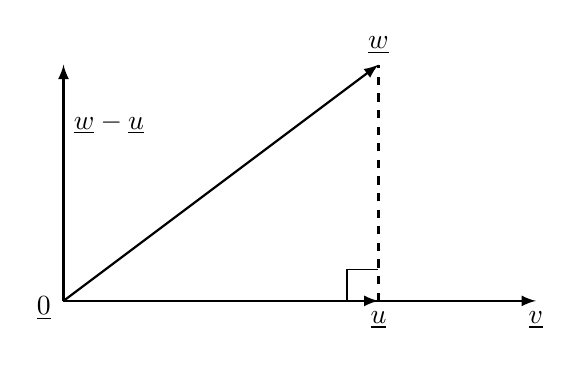
\begin{tikzpicture}
  \coordinate (v1) at (0,0);
  \coordinate (v2) at (4,3);
  \coordinate (v3) at (6,0);
  \coordinate (v4) at (4,0);
  \coordinate (v5) at (0,3);
  \path[draw] (3.6,0) -- (3.6,0.4) -- (4,0.4);
  \node (v0) at (-0.25,-0.1) {$\vecnot{0}$};
  \draw[-latex,thick] (v1) -- node[at end,above] {$\vecnot{w}$} (v2);
  \draw[-latex,thick] (v1) -- node[at end,below] {$\vecnot{v}$} (v3);
  \draw[-latex,thick] (v1) -- node[at end, below] {$\vecnot{u}$} (v4);
  \draw[thick,dashed] (v4) --  (v2);
  \draw[-latex,thick] (v1) -- node[right,near end] {$\vecnot{w}-\vecnot{u}$} (v5);
\end{tikzpicture}
\caption{\label{fig:vector_projection}The projection of $\vecnot{w}$ onto $\vecnot{v}$ is given by $\vecnot{u}$ and $\vecnot{w}-\vecnot{u}$ is orthogonal to $\vecnot{v}$.}
\end{figure}

\begin{definition}
Let $\vecnot{w},\vecnot{v}$ be vectors in an inner-product space $V$ with inner product $\tinner{ \cdot }{ \cdot }$.
As shown in Figure~\ref{fig:vector_projection}, the \defn{inner-product space}{projection} of $\vecnot{w}$ onto $\vecnot{v}$ is defined to be
\begin{equation*}
\vecnot{u} = \frac{\inner{ \vecnot{w} }{ \vecnot{v} }}{\|\vecnot{v}\|^2} \vecnot{v}
\end{equation*}
\end{definition}

\begin{lemma} \label{lem:proj_loss}
Let $\vecnot{u}$ be the projection of $\vecnot{w}$ onto $\vecnot{v}$.
Then, $\tinner{ \vecnot{w}-\vecnot{u} }{ \vecnot{u} } = 0$ and
\[ \|\vecnot{w}-\vecnot{u}\|^2 =  \|\vecnot{w}\|^2 - \| \vecnot{u} \|^2 = \|\vecnot{w}\|^2 - \frac{|\tinner{ \vecnot{w} }{ \vecnot{v} }|^2}{\|\vecnot{v}\|^2}. \]
\end{lemma}
\begin{proof}
First, we observe that
\[ \tinner{ \vecnot{w} - \vecnot{u} }{ \vecnot{v} } = \tinner{ \vecnot{w} }{ \vecnot{v} } - \tinner{ \vecnot{u} }{ \vecnot{v} } = \tinner{ \vecnot{w} }{ \vecnot{v} } - \frac{\inner{ \vecnot{w} }{ \vecnot{v} }}{\|\vecnot{v}\|^2} \tinner{ \vecnot{v} }{ \vecnot{v} } = 0. \]
Since $\vecnot{u} = s \vecnot{v}$ for some scalar $s$, we gather that $\tinner{ \vecnot{w}-\vecnot{u} }{ \vecnot{u} } = \tinner{ \vecnot{w}-\vecnot{u} }{ s \vecnot{v} } = \overline{s} \tinner{ \vecnot{w}-\vecnot{u} }{ \vecnot{v} } = 0$.
Using $\tinner{ \vecnot{w}-\vecnot{u} }{ \vecnot{u} } = 0$, we can write
\begin{align*}
\|\vecnot{w}\|^2 &= \|(\vecnot{w}-\vecnot{u})+\vecnot{u}\|^2
= \tinner{ (\vecnot{w}-\vecnot{u})+\vecnot{u}}{(\vecnot{w}-\vecnot{u})+\vecnot{u}} \\
&= \|\vecnot{w}-\vecnot{u}\|^2 + 2 \Real \tinner{ \vecnot{w}-\vecnot{u} }{ \vecnot{u} } + \|\vecnot{u}\|^2
= \|\vecnot{w}-\vecnot{u}\|^2 + \|\vecnot{u}\|^2.
\end{align*}
The proof is completed by noting that
$\|\vecnot{u}\|^2
= \frac{|\tinner{ \vecnot{w} }{ \vecnot{v} }|^2}{\|\vecnot{v}\|^4}
\tinner{ \vecnot{v} }{ \vecnot{v} }
= \frac{|\tinner{ \vecnot{w} }{ \vecnot{v} }|^2}{\|\vecnot{v}\|^2}$.
\end{proof}

\begin{theorem}
If $V$ is an inner-product space and $\| \cdot \|$ is its associated induced norm, then for any $\vecnot{v}, \vecnot{w} \in V$ and any scalar $s$
\begin{enumerate}
\item $\left\| s \vecnot{v} \right\| = |s| \left\| \vecnot{v} \right\|$
\item $\left\| \vecnot{v} \right\| > 0$ for $\vecnot{v} \neq \vecnot{0}$
\item $\left| \inner{ \vecnot{v} }{ \vecnot{w} } \right| \leq \left\| \vecnot{v} \right\| \left\| \vecnot{w} \right\|$ with equality iff $\vecnot{v} = \vecnot{0}$, $\vecnot{w}=\vecnot{0}$, or $\vecnot{v} = s \vecnot{w}$
\item $\left\| \vecnot{v} + \vecnot{w} \right\| \leq \left\| \vecnot{v} \right\| + \left\| \vecnot{w} \right\|$ with equality iff $\vecnot{v} = \vecnot{0}$, $\vecnot{w}=\vecnot{0}$, or $\vecnot{v} = s \vecnot{w}$.
\end{enumerate}
\end{theorem}
\begin{proof}
The first two properties follow immediately from the definitions involved.
The third property, $\left| \inner{ \vecnot{v} }{ \vecnot{w} } \right| \leq \left\| \vecnot{v} \right\| \left\| \vecnot{w} \right\|$, is called the \defn{inner-product space}{Cauchy-Schwarz inequality}.
When $\vecnot{v} = \vecnot{0}$, then clearly $\left| \inner{ \vecnot{v} }{ \vecnot{w} } \right| = \left\| \vecnot{v} \right\| \left\| \vecnot{w} \right\| =0$.
Assume $\vecnot{v} \neq \vecnot{0}$ and let
\begin{equation*}
\vecnot{u} = \frac{ \inner{ \vecnot{w} }{ \vecnot{v} }}{ \left\| \vecnot{v} \right\|^2 } \vecnot{v}
\end{equation*}
be the projection $\vecnot{w}$ onto $\vecnot{v}$.
By Lemma~\ref{lem:proj_loss},
we have
%$\inner{ \vecnot{w} - \vecnot{u} }{ \vecnot{v} } = 0$ and
\begin{align} \label{equation:DifferenceProjection}
0 &\leq \left\| \vecnot{w} - \vecnot{u} \right\|^2
%= \inner{ \vecnot{u} }{ \vecnot{w} - \frac{ \inner{ \vecnot{w} }{ \vecnot{v} }}{ \left\| \vecnot{v} \right\|^2 } \vecnot{v} } = \inner{ \vecnot{u} }{ \vecnot{w} }
%= \inner{ \vecnot{w} - \frac{ \inner{ \vecnot{w} }{ \vecnot{v} }}{ \left\| \vecnot{v} \right\|^2 } \vecnot{v} | \vecnot{w} } \\
%&= \inner{ \vecnot{w} }{ \vecnot{w} }
%- \frac{ \inner{ \vecnot{w} }{ \vecnot{v} }
%\inner{ \vecnot{v} }{ \vecnot{w} }}
%{ \left\| \vecnot{v} \right\|^2 }
= \left\| \vecnot{w} \right\|^2
- \frac{ \left| \inner{ \vecnot{w} }{ \vecnot{v} } \right|^2 }
{ \left\| \vecnot{v} \right\|^2 } ,
\end{align}
where equality holds iff $\vecnot{w}-\vecnot{u}=\vecnot{0}$, or equivalently iff $\vecnot{w}=\vecnot{0}$ or $\vecnot{v} = s \vecnot{w}$.
Rearranging \eqref{equation:DifferenceProjection} by isolating the inner product component and cross-multiplying, we find that
\begin{equation*}
\left| \inner{ \vecnot{v} }{ \vecnot{w} } \right|^2 = \left| \inner{ \vecnot{w} }{ \vecnot{v} } \right|^2 \leq \left\| \vecnot{v} \right\|^2 \left\| \vecnot{w} \right\|^2 .
\end{equation*}
%with equality iff $\vecnot{v}=\vecnot{0}$, $\vecnot{w}=\vecnot{0}$, or $\vecnot{v} = s \vecnot{w}$.
%Note that the $\vecnot{v}=\vecnot{0}$ case is checked separately because it is assumed above that $\vecnot{v}\neq \vecnot{0}$.
Using this result, we get the fourth property
\begin{equation*}
\begin{split}
\left\| \vecnot{v} + \vecnot{w} \right\|^2
&= \left\| \vecnot{v} \right\|^2 + \inner{ \vecnot{v} }{ \vecnot{w} } + \inner{ \vecnot{w} }{ \vecnot{v} } + \left\| \vecnot{w} \right\|^2 \\
&= \left\| \vecnot{v} \right\|^2 + 2 \Real \inner{ \vecnot{v} }{ \vecnot{w} } + \left\| \vecnot{w} \right\|^2 \\
&\leq \left\| \vecnot{v} \right\|^2 + 2 \left\| \vecnot{v} \right\| \left\| \vecnot{w} \right\| + \left\| \vecnot{w} \right\|^2 ,
\end{split}
\end{equation*}
with equality iff Cauchy-Schwarz holds with equality.
Thus, $\left\| \vecnot{v} + \vecnot{w} \right\| \leq \left\| \vecnot{v} \right\| + \left\| \vecnot{w} \right\|$ with equality iff $\vecnot{v} = \vecnot{0}$, $\vecnot{w}=\vecnot{0}$, or $\vecnot{v} = s \vecnot{w}$ (i.e., $\vecnot{v}$ and $\vecnot{w}$ are linearly dependent).
\end{proof}

%Its proof shows that if $\vecnot{v}$ is non-zero, then $\left| \inner{ \vecnot{v} }{ \vecnot{w} } \right| < \left\| \vecnot{v} \right\| \left\| \vecnot{w} \right\|$ unless
%\begin{equation*}
%\vecnot{w} = \frac{ \inner{ \vecnot{w} }{ \vecnot{v} } }
%{ \left\| \vecnot{v} \right\| } \vecnot{v} .
%\end{equation*}
%That is, equality holds if and only if $\vecnot{v}$ and $\vecnot{w}$ are linearly dependent.

\begin{theorem}
\label{theorem:InnerProductContinuous}
Consider the vector space $\RealNumbers^n$ with the standard inner product. % of Example~\ref{example:StandardInnerProduct}.
Then, the function $f \colon V \rightarrow F$ defined by $f \left( \vecnot{w} \right) = \inner{ \vecnot{w} }{ \vecnot{v} }$ is continuous.
\end{theorem}
\begin{proof}
Let $\vecnot{w}_1, \vecnot{w}_2, \ldots$ be a sequence in $V$ converging to $\vecnot{w}$.
Then,
\begin{equation*}
\left| \inner{ \vecnot{w}_n }{ \vecnot{v} }
- \inner{ \vecnot{w} }{ \vecnot{v} } \right|
= \left| \inner{ \vecnot{w}_n - \vecnot{w} }{ \vecnot{v} } \right|
\leq \left\| \vecnot{w}_n - \vecnot{w} \right\| \left\| \vecnot{v} \right\|.
\end{equation*}
Since $\left\| \vecnot{w}_n - \vecnot{w} \right\| \rightarrow 0$, the convergence of $\inner{ \vecnot{w}_n }{ \vecnot{v} }$ is established.
\end{proof}


\section{Sets of Orthogonal Vectors}

\begin{definition}
Let $V$ be an inner-product space and $U,W$ be subspaces.
Then, the subspace $U$ is an \defn{inner-product space}{orthogonal} to the subspace $W$ (denoted $U \bot W$) if $\vecnot{u} \bot \vecnot{w}$ for all $\vecnot{u}\in U$ and $\vecnot{w}\in W$.
\end{definition}

\begin{definition}
A collection $W$ of vectors in $V$ is an \defn{inner-product space}{orthogonal set} if all pairs of distinct vectors in $W$ are orthogonal.
\end{definition}

\begin{example}
The standard basis of $\RealNumbers^n$ is an orthonormal set with respect to the standard inner product.
\end{example}

\begin{example}
Let $V$ be the vector space (over $\ComplexNumbers$) of continuous complex-valued functions on the interval $0 \leq x \leq 1$ with the inner product
\begin{equation*}
\inner{ f }{ g } = \int_0^1 f(x) \overline{g(x)} dx.
\end{equation*}
Let $f_n(x) = \sqrt{2} \cos 2 \pi n x$ and $g_n (x) = \sqrt{2} \sin 2 \pi n x$.
Then $\{ 1, f_1, g_1, f_2, g_2, \ldots \}$ is a countably infinite orthonormal set that is a Schauder basis for this vector space.
\end{example}

\begin{theorem}
An orthogonal set of non-zero vectors is linearly independent.
\end{theorem}
\begin{proof}
Let $W$ be an orthogonal set of non-zero vectors in a given inner-product space $V$.
Suppose $\vecnot{w}_1, \ldots, \vecnot{w}_n$ are distinct vectors in $W$ and consider
\begin{equation*}
\vecnot{v} = s_1 \vecnot{w}_1 + \cdots + s_n \vecnot{w}_n.
\end{equation*}
The inner product $\inner{ \vecnot{v} }{ \vecnot{w}_i }$ is given by
\begin{equation*}
\begin{split}
\inner{ \vecnot{v} }{ \vecnot{w}_i }
&= \inner{ \sum_j s_j \vecnot{w}_j }{ \vecnot{w}_i }
= \sum_j s_j \inner{ \vecnot{w}_j }{ \vecnot{w}_i }
= s_i \inner{ \vecnot{w}_i }{ \vecnot{w}_i } .
\end{split}
\end{equation*}
Since $\inner{ \vecnot{w}_i }{ \vecnot{w}_i } \neq 0$, it follows that
\begin{equation*}
s_i = \frac{ \inner{ \vecnot{v} }{ \vecnot{w}_i } }
{ \left\| \vecnot{w}_i \right\|^2 }
\quad 1 \leq i \leq n.
\end{equation*}
In particular, if $\vecnot{v} = 0$ then $s_j = 0$ for $1 \leq j \leq n$ and the vectors in $W$ are linearly independent.
\end{proof}

\begin{corollary}
If $\vecnot{v} \in V$ is a linear combination of an orthogonal sequence of distinct, non-zero vectors $\vecnot{w}_1, \ldots, \vecnot{w}_n$, then $\vecnot{v}$ satisfies the identity
\begin{equation*}
\vecnot{v} = \sum_{i = 1}^n \frac{ \inner{ \vecnot{v} }{ \vecnot{w}_i } } { \left\| \vecnot{w}_i \right\|^2 } \vecnot{w}_i,
\end{equation*}
and equals the sum of the projections of $\vecnot{v}$ onto $\vecnot{w}_1, \ldots, \vecnot{w}_n$.
\end{corollary}

\begin{theorem}
Let $V$ be an inner-product space and assume $\vecnot{v}_1, \ldots, \vecnot{v}_n$ are linearly independent vectors in $V$.
Then it is possible to construct an orthogonal sequence of vectors $\vecnot{w}_1, \ldots, \vecnot{w}_n \in V$ such that for each $k = 1, \ldots, n$ the set
\begin{equation*}
\left\{ \vecnot{w}_1, \ldots, \vecnot{w}_k \right\}
\end{equation*}
is a basis for the subspace spanned by $\vecnot{v}_1, \ldots, \vecnot{v}_k$.
\end{theorem}
\begin{proof}
First, let $\vecnot{w}_1 = \vecnot{v}_1$.
The remaining vectors are defined inductively as part during the proof.
Suppose the vectors
\begin{equation*}
\vecnot{w}_1, \ldots, \vecnot{w}_m \quad (1 \leq m < n)
\end{equation*}
have been chosen so that for every $k$
\begin{equation*}
\left\{ \vecnot{w}_1, \ldots, \vecnot{w}_k \right\} \quad 1 \leq k \leq m
\end{equation*}
is an orthogonal basis for the subspace spanned by $\vecnot{v}_1, \ldots, \vecnot{v}_k$.
Let
\begin{equation*}
\vecnot{w}_{m+1} = \vecnot{v}_{m+1} - \sum_{i=1}^m \frac{ \inner{ \vecnot{v}_{m+1} }{ \vecnot{w}_i } } { \left\| \vecnot{w}_i \right\|^2 } \vecnot{w}_i.
\end{equation*}
Then $\vecnot{w}_{m+1} \neq 0$, for otherwise $\vecnot{v}_{m+1}$ is a linear combination of $\vecnot{w}_1, \ldots, \vecnot{w}_m$ and hence a linear combination of $\vecnot{v}_1, \ldots, \vecnot{v}_m$.
For $j \in \{1, \ldots, m\}$, we also have
\begin{equation*}
\begin{split}
\inner{ \vecnot{w}_{m+1} }{ \vecnot{w}_j }
&= \inner{ \vecnot{v}_{m+1} }{ \vecnot{w}_j }
- \sum_{i=1}^m \frac{ \inner{ \vecnot{v}_{m+1} }{ \vecnot{w}_i } } { \left\| \vecnot{w}_i \right\|^2 }
\inner{ \vecnot{w}_i }{ \vecnot{w}_j } \\
&= \inner{ \vecnot{v}_{m+1} }{ \vecnot{w}_j }
- \frac{ \inner{ \vecnot{v}_{m+1} }{ \vecnot{w}_j } } { \left\| \vecnot{w}_j \right\|^2 }
\inner{ \vecnot{w}_j }{ \vecnot{w}_j } \\
&= 0.
\end{split}
\end{equation*}
Clearly, $\{ \vecnot{w}_1, \ldots, \vecnot{w}_{m+1} \}$ is an orthogonal set consisting of $m+1$ non-zero vectors in the subspace spanned by $\vecnot{v}_1, \ldots, \vecnot{v}_{m+1}$.
Since the dimension of the latter subspace is $m+1$, this set is a basis for the subspace.
\end{proof}

The inductive construction of the vectors $\vecnot{w}_1, \ldots, \vecnot{w}_n$ is known as the \defn{inner-product space}{Gram-Schmidt orthogonalization} process.

\begin{corollary}
\label{cor:orthonormal_basis}
Every finite-dimensional inner-product space has a basis of orthonormal vectors.
\end{corollary}
\begin{proof}
Let $V$ be a finite-dimensional inner-product space.
Suppose that $\vecnot{v}_1, \ldots, \vecnot{v}_n$ is a basis for $V$.
Apply the Gram-Schmidt process to obtain a basis of orthogonal vectors $\vecnot{w}_1, \ldots, \vecnot{w}_n$.
Then, a basis of orthonormal vectors is given by
\begin{equation*}
\vecnot{u}_1 = \frac{ \vecnot{w}_1 }{ \left\| \vecnot{w}_1 \right\| }, \ldots,
\vecnot{u}_n = \frac{ \vecnot{w}_n }{ \left\| \vecnot{w}_n \right\| }.
\end{equation*}
\end{proof}

\begin{example}
Consider the vectors
\begin{align*}
\vecnot{v}_1 &= (2,2,1) \\
\vecnot{v}_2 &= (3,6,0) \\
\vecnot{v}_3 &= (6,3,9)
\end{align*}
in $\RealNumbers^3$ equipped with the standard inner product.
Apply the Gram-Schmidt process to $\vecnot{v}_1, \vecnot{v}_2, \vecnot{v}_3$ to obtain an orthogonal basis.

Applying the Gram-Schmidt process to $\vecnot{v}_1, \vecnot{v}_2, \vecnot{v}_3$, we get
\begin{align*}
\vecnot{w}_1 &= (2,2,1) \\
\vecnot{w}_2 &= (3,6,0)
- \frac{ \inner{ (3,6,0) }{ (2,2,1) } }{ 9 } (2,2,1) \\
&= (3,6,0) - 2 (2,2,1) = (-1,2,-2) \\
\vecnot{w}_3 &= (6,3,9)
- \frac{ \inner{ (6,3,9) }{ (2,2,1) } }{ 9 } (2,2,1)
- \frac{ \inner{ (6,3,9) }{ (-1,2,-2) } }{ 9 } (-1,2,-2) \\
&= (6,3,9) - 3 (2,2,1) + 2 (-1,2,-2) = (-2,1,2) .
\end{align*}
It is easily verified that $\vecnot{w}_1, \vecnot{w}_2, \vecnot{w}_3$ is an orthogonal set of vectors.
\end{example}

\begin{definition}
Let $V$ be an inner-product space and $W$ be any set of vectors in $V$.
The \defn{inner-product space}{orthogonal complement} of $W$ denoted by $W^{\bot}$ is the set of all vectors in $V$ that are orthogonal to every vector in $W$ or
\begin{equation*}
W^{\bot} = \left\{ \vecnot{v} \in V \big| \tinner{ \vecnot{v} }{ \vecnot{w} } = 0 \; \forall \; \vecnot{w}\in W \right\}. 
\end{equation*}
\end{definition}

\begin{problem} \label{problem:WbotSubspace}
Let $W$ be any subset of vector space $V$.
Show that $W^{\bot}$ is a closed subspace of $V$ and that any vector in the subspace spanned by $W$ is orthogonal to any vector in $W^{\bot}$.
\end{problem}
\noindent
\textbf{S~\ref{problem:WbotSubspace}}.
Let $\vecnot{m}_1, \vecnot{m}_2 \in W^{\bot}$ and $s \in F$.
For any vector $\vecnot{w} \in W$, we have
\begin{equation*}
\inner{ \vecnot{m}_1 }{ \vecnot{w} }
= \inner{ \vecnot{m}_2 }{ \vecnot{w} }
= 0.
\end{equation*}
This implies
\begin{equation*}
\inner{ s \vecnot{m}_1 + \vecnot{m}_2 }{ \vecnot{w} }
= s \inner{ \vecnot{m}_1 }{ \vecnot{w} }
+ \inner{ \vecnot{m}_2 }{ \vecnot{w} }
= 0.
\end{equation*}
That is, $s \vecnot{m}_1 + \vecnot{m}_2 \in W^{\bot}$.
Hence, $W^{\bot}$ is a subspace of $V$.

To see that $W^{\bot}$ is closed, we let $\vecnot{m}$ be any point in the closure of $W^{\bot}$ and $\vecnot{m}_1,\vecnot{m}_2,\ldots \in W^{\bot}$ be a sequence that converges to $\vecnot{m}$.
The continuity of the inner product, from Theorem~\ref{theorem:InnerProductContinuous}, implies that, for all $\vecnot{w}\in W$,
\[ \inner{ \vecnot{m} }{ \vecnot{w} } =  \inner{ \lim_{n\rightarrow\infty} \vecnot{m}_n }{ \vecnot{w}  }  =  \lim_{n\rightarrow\infty}  \inner{ \vecnot{m}_n }{ \vecnot{w}  } = 0. \]
Therefore, $\vecnot{m} \in W^{\bot}$ and the orthogonal complement contains all of its limit points.

Notice also that any vector $\vecnot{w}$ in the subspace spanned by $W$ can be written as $\vecnot{w} = \sum_{i} s_i \vecnot{w}_i$ with $\vecnot{w}_i \in W$ and $s_i \in F$.
Therefore, the inner product of $\vecnot{w}$ with any $\vecnot{w}' \in W^{\bot}$ is given by
\begin{equation*}
\inner{ \vecnot{w} }{ \vecnot{w}' }
= \inner{ \sum_{i} s_i \vecnot{w}_i }{ \vecnot{w}' } \\
= \sum_{i} s_i \inner{ \vecnot{w}_i }{ \vecnot{w}' } \\
= 0.
\end{equation*}
It follows that the subspace spanned by $W$ is orthogonal to the subspace $W^{\bot}$.

\begin{definition}
A complex matrix $U\in \ComplexNumbers^{n\times n}$ is called \defn{inner-product space}{unitary} if $U^H U = I$.
Similarly, a real matrix $Q\in \RealNumbers^{n\times n}$ is called \defn{inner-product space}{orthogonal} if $Q^T Q = I$.
\end{definition}

\begin{theorem}
Let $V = \ComplexNumbers^n$ be the standard inner product space and let  $U\in \ComplexNumbers^{n\times n}$ define a linear operator on $V$.
Then, the following conditions are equivalent:
\begin{enumerate}
\item[(i)] The columns of $U$ form an orthonormal basis (i.e.,  $U^H U = I$),
\item[(ii)] the rows of $U$ form an orthonormal basis (i.e.,  $U U^H = I$),
\item[(iii)] $U$ preserves inner products (i.e., $\tinner{ U \vecnot{v} }{ U \vecnot{w} } = \tinner{ \vecnot{v} }{ \vecnot{w} }$ for all $\vecnot{u},\vecnot{v}\in V$), and
\item[(iv)] $U$ is an isometry (i.e., $\| U \vecnot{v} \| = \| \vecnot{v}\|$ for all $\vecnot{v} \in V$).
\end{enumerate}
\end{theorem}
\begin{proof}
If {\it(i)} holds, then $U$ is invertible because its columns are linearly independent.
Thus, $U^H U = I$ implies $U^H = U^{-1}$ and {\it(ii)} follows.
Likewise, {\it(iii)} holds because $\tinner{ U \vecnot{v} }{ U \vecnot{w} } = \vecnot{w}^H U^H U \vecnot{v} = \vecnot{w}^H \vecnot{v} = \tinner{ \vecnot{v} }{ \vecnot{w} }$ for all $\vecnot{u},\vecnot{v}\in V$.
Choosing $\vecnot{w}=\vecnot{v}$ gives {\it(iv)}.
Lastly, if $\| U \vecnot{v} \| = \| \vecnot{v}\|$ for all $\vecnot{v} \in V$, then
$\vecnot{v}^H (U^H U - I) \vecnot{v} = \| U \vecnot{v} \|^2 - \| \vecnot{v} \|^2 = 0$ for all $\vecnot{v} \in V$.
Since $U^H U - I$ is Hermitian, it must have a complete set of eigenvectors but all eigenvalues must be 0.  Thus, $U^H U - I = 0$.
\end{proof}

\subsection{Hilbert Spaces}

\begin{definition}
A complete inner-product space is called a \defn{inner-product space}{Hilbert space}.
\end{definition}

\begin{definition}
Recall that a subset $\left\{ \vecnot{v}_{\alpha} | \alpha \in A \right\}$ of a Hilbert space $V$ is said to be orthonormal if $\left\| \vecnot{v}_{\alpha} \right\| = 1$ for every $\alpha \in A$ and $\inner{ \vecnot{v}_{\alpha} }{ \vecnot{v}_{\beta} } = 0$ for all $\alpha \neq \beta$.
If the subspace spanned by the family $\left\{ \vecnot{v}_{\alpha} | \alpha \in A \right\}$ is dense in $V$, we call this set an \defn{inner-product space}{orthonormal basis}.
\end{definition}

Note that, according to this definition, an orthonormal basis for a Hilbert space $V$ is not necessarily a Hamel basis for $V$.
However, it can be shown that any orthogonal basis is a subset of a Hamel basis.
In practice it is the orthonormal basis, not the Hamel basis itself, which is of most use.
None of these issues arise in finite-dimensional spaces, where an orthogonal basis is always a Hamel basis.

Let $\mathcal{B} = \left\{ \vecnot{v}_{\alpha} | \alpha \in A \right\}$ be an orthonormal basis for Hilbert space $V$.
Then, each element $\vecnot{v} \in V$ has a unique representation as
\begin{equation*}
\vecnot{v} = \sum_{\alpha \in A} s_{\alpha} \vecnot{v}_{\alpha}.
\end{equation*}
Using orthogonality to compute $\inner{ \vecnot{v} }{ \vecnot{v} }$, one gets the \defn{inner-product space}{Parseval identity}
\begin{equation*}
\left\| \vecnot{v} \right\|^2 = \sum_{\alpha \in A} | s_{\alpha} |^2.
\end{equation*}
Since $\| \vecnot{v} \|^2 < \infty$ for all $\vecnot{v} \in V$, the RHS also exists and is finite for all $\vecnot{v} \in V$.

\begin{theorem}
Every orthonormal set in a Hilbert space $V$ can be enlarged to an orthonormal basis for $V$.
\end{theorem}
\begin{proof}
Let $x = \left\{ \vecnot{v}_{\alpha} | \alpha \in A_0 \right\}$ be the initial orthonormal set.
Let $X$ be the set of orthonormal subsets of $V$ and, for $x, y \in X$, consider the strict partial order defined by proper inclusion.
Since $x$ is an element of $X$, the Hausdorff maximal principle implies that there exists a maximal simply ordered subset $Z$ of $X$ containing $x$.
This shows the existence of a maximal orthonormal set $\left\{ \vecnot{v}_{\alpha} | \alpha \in A \right\}$, where $A_0 \subset A$.

Let $W$ be the closed subspace of $V$ generated by $\left\{ \vecnot{v}_{\alpha} | \alpha \in A \right\}$.
If $W \neq V$, there is a unit vector $\vecnot{u} \in W^{\bot}$, contradicting the maximality of the system $\left\{ \vecnot{v}_{\alpha} | \alpha \in A \right\}$.
Thus, $W = V$ and we have enlarged the orthonormal set $x$ to a basis.
\end{proof}

\begin{theorem} \label{theorem:SeparableHilbertSpace}
A Hilbert space $V$ has a countable orthonormal basis if and only if $V$ is separable.
\end{theorem}
\begin{proof}[Sketch of proof]
If $V$ is separable, then it contains a countable dense subset.
Since this set is countable, it can be ordered into a sequence $\vecnot{v}_1 , \vecnot{v}_2 , \ldots$ such that, for every vector $\vecnot{v}\in V$ and any $\epsilon>0$, there exists an $n$ such that $\left\| \vecnot{v} - \vecnot{v}_n \right\| < \epsilon$.
By removing all vectors that are linear combinations of previous vectors, this sequence can be pruned into a countable linearly independent set.
Then, a countable orthonormal basis is generated by applying Gram-Schmidt orthogonalization to the pruned sequence of vectors.
Conversely, if $V$ has a countable orthonormal basis, then linear combinations with rational coefficients can be used to construct a countable dense subset.
\end{proof}

\begin{lemma} \label{lem:hilbert_sum_convergence}
Let $V$ be a Hilbert space and $\vecnot{v_1},\vecnot{v}_2,\ldots$ be a countable orthogonal set.
Then, $\vecnot{v} = \sum_{i=1}^\infty \vecnot{v}_i$ exists if and only $\sum_{i=1}^\infty \|\vecnot{v}_i\|^2 = M < \infty$.
\end{lemma}
\begin{proof}
For $\vecnot{u}_n = \sum_{i=1}^n \vecnot{v}_i$ and $w_n = \sum_{i=1}^n \|\vecnot{v}_i\|^2$, orthogonality implies that
\[\|\vecnot{u}_m - \vecnot{u}_n\|^2 = \left\| \sum_{i=n+1}^m \vecnot{v}_i \right\|^2 = \sum_{i=n+1}^m \|\vecnot{v}_i \|^2 = | w_m - w_n|. \]
Thus, the sequence $\vecnot{u}_n$ is Cauchy in $V$ if and only if $w_n$ is Cauchy in $\RealNumbers$.
\end{proof}


\section{Linear Functionals}

\begin{definition}
Let $V$ be a vector space over a field $F$.
A linear transformation $f$ from $V$ into the scalar field $F$ is called a \defn{vector space}{linear functional} on $V$.
\end{definition}
That is, $f$ is a functional on $V$ such that
\begin{equation*}
f \left( s \vecnot{v}_1 + \vecnot{v}_2 \right)
= s f \left( \vecnot{v}_1 \right) + f \left( \vecnot{v}_2 \right)
\end{equation*}
for all $\vecnot{v}_1, \vecnot{v}_2 \in V$ and $s \in F$.

\begin{example}
Let $F$ be a field and let $s_1, \ldots, s_n$ be scalars in $F$.
Then the functional $f$ on $F^n$ defined by
\begin{equation*}
f(v_1, \ldots, v_n) = s_1 v_1 + \cdots + s_n v_n
\end{equation*}
is a linear functional.
It is the linear functional which is represented by the matrix
\begin{equation*}
\begin{bmatrix} s_1 & s_2 & \cdots & s_n \end{bmatrix}
\end{equation*}
relative to the standard ordered basis for $F^n$.
Every linear functional on $F^n$ is of this form, for some scalars $s_1, \ldots, s_n$.
\end{example}

\begin{definition}
Let $n$ be a positive integer and $F$ a field.
If $A$ is an $n \times n$ matrix with entries in $F$, the \defn{matrix}{trace} of $A$ is the scalar
\begin{equation*}
\Trace(A) = A_{11} + A_{22} + \cdots + A_{nn}.
\end{equation*}
\end{definition}

\begin{example}
The trace function is a linear functional on the matrix space $F^{n \times n}$ since
\begin{equation*}
\begin{split}
\Trace ( sA + B) &= \sum_{i=1}^n (s A_{ii} + B_{ii}) \\
&= s \sum_{i=1}^n A_{ii} + \sum_{i=1}^n  B_{ii} \\
&= s \; \Trace(A) + \Trace(B) .
\end{split}
\end{equation*}
\end{example}

\begin{example}
Let $[a, b]$ be a closed interval on the real line and let $C([a,b])$ be the space of continuous real-valued functions on $[a,b]$.
Then
\begin{equation*}
L(g) = \int_a^b g(t) dt
\end{equation*}
defines a linear functional $L$ on $C([a,b])$.
\end{example}

\begin{theorem}[Riesz] \label{theorem:riesz_finite}
Let $V$ be a finite-dimensional Hilbert space and $f$ be a linear functional on $V$.
Then, there exists a unique vector $\vecnot{v} \in V$ such that $f \left( \vecnot{w} \right) = \inner{ \vecnot{w} }{ \vecnot{v} }$ for all $\vecnot{w} \in V$.
\end{theorem}

\begin{proof}
%Now, we can take a closer look at the proof of this theorem for the finite dimensional case.
If we choose an orthonormal basis $\mathcal{B} = \vecnot{v}_1, \ldots, \vecnot{v}_n$ for $V$, then the inner product of $\vecnot{w} = t_1 \vecnot{v}_1 + \cdots + t_n \vecnot{v}_n$ and $\vecnot{v} = s_1 \vecnot{v}_1 + \cdots + s_n \vecnot{v}_n$ will be
\begin{equation*}
\inner{ \vecnot{w} }{ \vecnot{v} } = t_1 \bar{s}_1 + \cdots + t_n \bar{s}_n .
\end{equation*}
If $f$ is a linear functional on $V$, then $f$ has the form
\begin{equation*}
f \left(\vecnot{w}\right) = f(t_1 \vecnot{v}_1 + \cdots + t_n \vecnot{v}_n) = t_1 f \left( \vecnot{v}_1 \right) + \cdots + t_n f \left( \vecnot{v}_n \right).
\end{equation*}
Thus, we can choose $\bar{s}_j = f \left( \vecnot{v}_j \right)$ to get $ \inner{ \vecnot{w} }{ \vecnot{v} } = f \left( \vecnot{w} \right)$ and this gives
\begin{equation*}
\vecnot{v} = \overline{ f \left( \vecnot{v}_1 \right) } \vecnot{v}_1 + \cdots + \overline{ f \left( \vecnot{v}_n \right) } \vecnot{v}_n .
\end{equation*}

Let $\vecnot{v}'$ be any vector that satisfies $f \left( \vecnot{w} \right) = \inner{ \vecnot{w} }{ \vecnot{v}' }$ for all $\vecnot{w}\in V$.
Then, we see that $\inner{ \vecnot{w} }{ \vecnot{v} - \vecnot{v}' } = 0$
for all $\vecnot{w}\in V$.
This implies that $\vecnot{v}-\vecnot{v}' = \vecnot{0}$.

\iffalse

Thus, the vector $\vecnot{v}$ is unique.
 for some fixed scalars $c_1, \ldots, c_n$ determined by the basis.
Clearly, $f \left( \vecnot{v}_j \right) = c_j$, which implies that $\bar{s}_j = f \left( \vecnot{v}_j \right)$.
That is, the vector $\vecnot{v}$ such that $f \left( \vecnot{w} \right) = \inner{ \vecnot{w} }{ \vecnot{v} }$ is

Note that the vector $\vecnot{v}$ lies in the orthogonal complement of the nullspace of $f$.
Let $W$ be the nullspace of $f$, then $V = W \oplus W^{\bot}$, and $f$ is completely determined by its value on $W^{\bot}$.
In fact, if $P$ gives the orthogonal projection of $V$ on $W^{\bot}$, then
\begin{equation*}
f \left( \vecnot{u} \right) = f \left( P \vecnot{u} \right)
\end{equation*}
for all $\vecnot{u} \in V$.
Suppose that $f \neq 0$, then $f$ is of rank one and $\dim \left( W^{\bot} \right) = 1$.
If $\vecnot{v}$ is any non-zero vector in $W^{\bot}$, it follows that
\begin{equation*}
P \vecnot{u} = \frac{ \inner{ \vecnot{u} }{ \vecnot{v} } }{ \left\| \vecnot{v} \right\|^2 } \vecnot{v}
\end{equation*}
for all $\vecnot{u} \in V$.
Thus,
\begin{equation*}
f \left( \vecnot{u} \right) = \inner{ \vecnot{u} }{ \vecnot{v} }
\frac{f \left( \vecnot{v} \right) }{ \left\| \vecnot{v} \right\|^2 }
\end{equation*}
for all $\vecnot{u} \in V$.
\fi

\end{proof}

\chapter{Representations and Approximations}

\section{Best Approximation}

Orthogonal projections are very useful in many contexts.
In essence, the Gram-Schmidt process is a sequence of orthogonal projections.

Suppose $W$ is a subspace of an inner-product space $V$, and let $\vecnot{v}$ be an arbitrary vector in $V$.
Consider the problem of finding a vector $\vecnot{w} \in W$ such that $\left\| \vecnot{v} - \vecnot{w} \right\|$ is minimized.
The vector $\vecnot{w} \in W$ is a \defn{inner-product space}{best approximation} to $\vecnot{v} \in V$ if
\begin{equation*}
\left\| \vecnot{v} - \vecnot{w} \right\| \leq \left\| \vecnot{v} - \vecnot{w}' \right\|
\end{equation*}
for every vector $\vecnot{w}' \in W$.

\begin{theorem} \label{theorem:OrthogonalProjection}
Suppose $W$ is a subspace of an inner-product space $V$, and let $\vecnot{v}$ be a vector in $V$.
\begin{enumerate}
\item The vector $\vecnot{w} \in W$ is a best approximation of $\vecnot{v} \in V$ by vectors in $W$ if and only if $\vecnot{v} - \vecnot{w}$ is orthogonal to every vector in $W$.
\item If a best approximation to $\vecnot{v} \in V$ by vectors in $W$ exists, it is unique.
\item If $W$ is finite-dimensional and $\vecnot{w}_1, \ldots, \vecnot{w}_n$ is an orthogonal basis for $W$, then
\begin{equation*}
\vecnot{w} = \sum_{i=1}^n \frac{ \left\langle \vecnot{v} | \vecnot{w}_i \right\rangle }{ \left\| \vecnot{w}_i \right\|^2 } \vecnot{w}_i
\end{equation*}
is the best approximation to $\vecnot{v}$ by vectors in $W$.
\end{enumerate}
\end{theorem}
\begin{proof}
Let $\vecnot{w} \in W$ and suppose $\vecnot{v} - \vecnot{w}$ is orthogonal to every vector in $W$.
Let $\vecnot{w}' \in W$ such that $\vecnot{w}' \neq \vecnot{w}$.
Then $\vecnot{v} - \vecnot{w}' = \left( \vecnot{v} - \vecnot{w} \right) + \left( \vecnot{w} - \vecnot{w}' \right)$ and
\begin{equation} \label{equation:OrthogonalVector}
\begin{split}
\left\| \vecnot{v} - \vecnot{w}' \right\|^2
&= \left\| \vecnot{v} - \vecnot{w} \right\|^2
+ 2 \Real \left\langle \vecnot{v} - \vecnot{w} | \vecnot{w} - \vecnot{w}' \right\rangle
+ \left\| \vecnot{w} - \vecnot{w}' \right\|^2 \\
&= \left\| \vecnot{v} - \vecnot{w} \right\|^2
+ \left\| \vecnot{w} - \vecnot{w}' \right\|^2 \\
&\geq \left\| \vecnot{v} - \vecnot{w} \right\|^2.
\end{split}
\end{equation}
Conversely, suppose that $\left\| \vecnot{v} - \vecnot{w}' \right\| \geq \left\| \vecnot{v} - \vecnot{w} \right\|$ for every $\vecnot{w}' \in W$.
From \eqref{equation:OrthogonalVector}, we get
\begin{equation*}
2 \Real \left\langle \vecnot{v} - \vecnot{w} | \vecnot{w} - \vecnot{w}' \right\rangle
+ \left\| \vecnot{w} - \vecnot{w}' \right\|^2 \geq 0
\end{equation*}
for all $\vecnot{w}' \in W$.
Note that every vector in $W$ can be expressed as $\vecnot{w} - \vecnot{w}'$ where $\vecnot{w}' \in W$, it follows that
\begin{equation} \label{equation:InequalityOrthogonalVectors}
2 \Real \left\langle \vecnot{v} - \vecnot{w} | \vecnot{w}'' \right\rangle
+ \left\| \vecnot{w}'' \right\|^2 \geq 0
\end{equation}
for every $\vecnot{w}'' \in W$.
If $\vecnot{w}'$ is in $W$ and $\vecnot{w}' \neq \vecnot{w}$ then we may take
\begin{equation*}
\vecnot{w}'' = - \frac{ \left\langle \vecnot{v} - \vecnot{w} | \vecnot{w} - \vecnot{w}' \right\rangle }{ \left\| \vecnot{w} - \vecnot{w}' \right\|^2 } \left( \vecnot{w} - \vecnot{w}' \right).
\end{equation*}
Inequality~\eqref{equation:InequalityOrthogonalVectors} then reduces to the statement
\begin{equation*}
- 2 \frac{ \left| \left\langle \vecnot{v} - \vecnot{w} | \vecnot{w} - \vecnot{w}' \right\rangle \right|^2 }{ \left\| \vecnot{w} - \vecnot{w}' \right\|^2 }
+ \frac{ \left| \left\langle \vecnot{v} - \vecnot{w} | \vecnot{w} - \vecnot{w}' \right\rangle \right|^2 }{ \left\| \vecnot{w} - \vecnot{w}' \right\|^2 }
\geq 0.
\end{equation*}
This inequality holds if and only if $\left\langle \vecnot{v} - \vecnot{w} | \vecnot{w} - \vecnot{w}' \right\rangle = 0$.
Therefore, $\vecnot{v} - \vecnot{w}$ is orthogonal to every vector in $W$.
Hence the vector $\vecnot{w} \in W$ is a best approximation of $\vecnot{v} \in V$ by vectors in $W$ if and only if $\vecnot{v} - \vecnot{w}$ is orthogonal to every vector in $W$.

Suppose $\vecnot{w}, \vecnot{w}' \in W$ are best approximations of $\vecnot{v}$ by vectors in $W$.
Then $\left\| \vecnot{v} - \vecnot{w} \right\| = \left\| \vecnot{v} - \vecnot{w}' \right\|$ and \eqref{equation:OrthogonalVector} implies that $\left\| \vecnot{w} - \vecnot{w}' \right\| = 0$.
That is, if a best approximation exists then it is unique.

Assume that $W$ is finite-dimensional and let $\vecnot{w}_1, \ldots, \vecnot{w}_n$ be an orthonormal basis for $W$.
Furthermore, let
\begin{equation*}
\vecnot{w} = \sum_{i=1}^n \frac{ \left\langle \vecnot{v} | \vecnot{w}_i \right\rangle }{ \left\| \vecnot{w}_i \right\|^2 } \vecnot{w}_i .
\end{equation*}
Then $\vecnot{v} -\vecnot{w}$ is orthogonal to $\vecnot{w}_j$ for $j = 1, \ldots, n$, i.e.,
\begin{equation*}
\begin{split}
\left\langle \vecnot{v} - \vecnot{w} | \vecnot{w}_j \right\rangle
&= \left\langle \vecnot{v} | \vecnot{w}_j \right\rangle
- \left\langle \sum_{i=1}^n \frac{ \left\langle \vecnot{v} | \vecnot{w}_i \right\rangle }{ \left\| \vecnot{w}_i \right\|^2 } \vecnot{w}_i \Big| \vecnot{w}_j \right\rangle \\
&= \left\langle \vecnot{v} | \vecnot{w}_j \right\rangle
- \frac{ \left\langle \vecnot{v} | \vecnot{w}_j \right\rangle }{ \left\| \vecnot{w}_i \right\|^2 } \left\langle \vecnot{w}_j | \vecnot{w}_j \right\rangle
= 0.
\end{split}
\end{equation*}
That is, $\vecnot{v} - \vecnot{w}$ is orthogonal to every vector in $W$ and therefore $\vecnot{w}$ is the best approximation to $\vecnot{v}$ by vectors in $W$.
\end{proof}

\begin{definition}
Whenever the vector $\vecnot{w}$ in Theorem~\ref{theorem:OrthogonalProjection} exists, it is equal to the \emph{orthogonal projection of $\vecnot{v}$ onto $W$}.
If every vector in $V$ has an orthogonal projection onto $W$, then we can define a mapping $E: V \rightarrow W$ that assigns to each vector in $V$ its orthogonal projection onto $W$ is called the \emph{orthogonal projection of $V$ onto $W$}.
\end{definition}

\begin{problem}
Let $W$ be the subspace of $\RealNumbers^2$ spanned by the vector $(1,2)$.
Using the standard inner product, let $E$ be the orthogonal projection of $\RealNumbers^2$ onto $W$.
Find
\begin{enumerate}
\item a formula for $E(x_1, x_2)$
\item the matrix of $E$ in the standard ordered basis, i.e., $E(x_1, x_2) = E \vecnot{x}$
\item $W^{\bot}$
\item an orthonormal basis in which $E$ is represented by the matrix
\begin{equation*}
E = \left[ \begin{array}{cc} 1 & 0 \\ 0 & 0 \end{array} \right].
\end{equation*}
\end{enumerate}
\end{problem}

\begin{corollary}
Let $V$ be an inner-product space, $W$ be a finite-dimensional subspace, and $E$ be the orthogonal projection of $V$ on $W$.
Then the mapping
\begin{equation*}
\vecnot{v} \mapsto \vecnot{v} - E \vecnot{v}
\end{equation*}
is the orthogonal projection of $V$ on $W^{\bot}$.
\end{corollary}
\begin{proof}
Let $\vecnot{v}$ be any vector in $V$.
Then, $\vecnot{v} - E\vecnot{v}$ is in $W^{\bot}$, and for any $\vecnot{u}$ in $W^{\bot}$, $\vecnot{v} - \vecnot{u} = E \vecnot{v} + \left( \vecnot{v} - E \vecnot{v} - \vecnot{u} \right)$.
Since $E \vecnot{v} \in W$ and $\vecnot{v} - E \vecnot{v} - \vecnot{u} \in W^{\bot}$, it follows that
\begin{equation*}
\begin{split}
\left\| \vecnot{v} - \vecnot{u} \right\|^2 &= \left\| E \vecnot{v} \right\|^2 + \left\| \vecnot{v} - E \vecnot{v} - \vecnot{u} \right\|^2 \\
&\geq \left\| \vecnot{v} - \left( \vecnot{v} - E \vecnot{v} \right) \right\|^2
\end{split}
\end{equation*}
with strict inequality when $\vecnot{u} \neq \vecnot{v} - E \vecnot{v}$.
Thus, $\vecnot{v} - E \vecnot{v}$ is the best approximation to $\vecnot{v}$ by vectors in $W^{\bot}$.
\end{proof}

\begin{theorem} \label{theorem:OrthogonalSubspaceDirectSum}
Suppose $V$ is an inner-product space.
Let $W$ be a finite-dimensional subspace of $V$ and let $E$ denote the orthogonal projection of $V$ on $W$.
Then $E$ is an idempotent linear transformation of $V$ onto $W$, $E \vecnot{w}' = \vecnot{0}\,$ iff $\vecnot{w}' \in W^{\bot}$, and
\begin{equation*}
V = W \oplus W^{\bot}.
\end{equation*}
\end{theorem}
\begin{proof}
Let $\vecnot{v}$ be any vector in $V$.
Then $E \vecnot{v}$ is the best approximation of $\vecnot{v}$ by vectors in $W$.
If $\vecnot{v} \in W$ then $E \vecnot{v} = \vecnot{v}$.
It follows that $E \left( E \vecnot{v} \right) = E \vecnot{v}$ for any $\vecnot{v} \in V$ since $E \vecnot{v} \in W$.
That is, $E^2 = E$ and $E$ is idempotent.

To show that $E$ is a linear transformation, let $\{ \vecnot{w}_1 , \vecnot{w}_2 , \ldots , \vecnot{w}_n \}$ be an orthonormal basis for $W$ (whose existence follows from Corollary~\ref{cor:orthonormal_basis}).
Using part 3 of Theorem~\ref{theorem:OrthogonalProjection}, we find that
\begin{align*}
E \left( s_1 \vecnot{v}_1 + \vecnot{v}_2 \right)
& = \sum_{i=1}^n \langle  s_1 \vecnot{v}_1 + \vecnot{v}_2 | \vecnot{w}_i \rangle \vecnot{w}_i \\
& = s_1 \sum_{i=1}^n \langle  \vecnot{v}_1 | \vecnot{w}_i \rangle \vecnot{w}_i + \sum_{i=1}^n \langle  \vecnot{v}_2 | \vecnot{w}_i \rangle \vecnot{w}_i \\
& = s_1 E \vecnot{v}_1 + E \vecnot{v}_2.
\end{align*}
Therefore, $E$ is a linear transformation.
It also follows that $E \vecnot{w}' = \vecnot{0}$ iff $\vecnot{w}' \in W^{\bot}$ because $W^{\bot}$ can be defined by the fact that $\langle \vecnot{w}' | \vecnot{w}_i \rangle = 0$ for $i=1,2,\ldots,n$.

\iffalse
To show that $E$ is a linear transformation, consider vectors $\vecnot{v}_1, \vecnot{v}_2 \in V$ and scalar $s \in F$.
Then $\vecnot{v}_1 - E \vecnot{v}_1$ and $\vecnot{v}_2 - E \vecnot{v}_2$ are each orthogonal to every vector in $W$.
The vector
\begin{equation*}
s \left( \vecnot{v}_1 - E \vecnot{v}_1 \right) + \left( \vecnot{v}_2 - E \vecnot{v}_2 \right) = \left( s \vecnot{v}_1 + \vecnot{v}_2 \right) - \left( s E \vecnot{v}_1 + E \vecnot{v}_2 \right)
\end{equation*}
is therefore also orthogonal to every vector in $W$.
Since $s E \vecnot{v}_1 + E \vecnot{v}_2$ is a vector in $W$, it follows from Theorem~\ref{theorem:OrthogonalProjection} that
\begin{equation*}
E \left( s \vecnot{v}_1 + \vecnot{v}_2 \right) = s E \vecnot{v}_1 + E \vecnot{v}_2.
\end{equation*}
That is, $E$ is a linear transformation.

Again, let $\vecnot{v} \in V$.
Then $E \vecnot{v}$ is the unique vector in $W$ such that $\vecnot{v} - E \vecnot{v}$ is in $W^{\bot}$.
In particular, $E \vecnot{v} = \vecnot{0}$ when $\vecnot{v} \in W^{\bot}$.
Conversely, if $E \vecnot{v} = \vecnot{0}$ then $\vecnot{v} \in W^{\bot}$.
Thus $W^{\bot}$ is the nullspace of $E$.
The equation
\begin{equation*}
\vecnot{v} = E \vecnot{v} + \vecnot{v} - E \vecnot{v}
\end{equation*}
shows that $V = W + W^{\bot}$.
Furthermore, $W \cap W^{\bot} = \left\{ \vecnot{0} \right\}$.
Hence $V$ is the direct sum of $W$ and $W^{\bot}$.
\fi

Again, let $\vecnot{v} \in V$ and recall that (by Theorem~\ref{theorem:OrthogonalProjection}) $E \vecnot{v}$ is the unique vector in $W$ such that $\vecnot{v} - E \vecnot{v}$ is in $W^{\bot}$.
Therefore, the equation $\vecnot{v} = E \vecnot{v} + \left( \vecnot{v} - E \vecnot{v} \right)$ gives a unique decomposition of $\vecnot{v}$ into $E \vecnot{v} \in W$ and $\vecnot{v} - E \vecnot{v} \in W^{\bot}$.
This unique decomposition implies that $V$ is the direct sum of $W$ and $W^{\bot}$.
Of course, from the definition of $W^{\bot}$ it follows that
\[W \cap W^{\bot} = \left\{ \vecnot{u} \in W | \langle \vecnot{u} | \vecnot{w} \rangle =0 \; \forall \; \vecnot{w}\in W \right\}  \subseteq \left\{ \vecnot{u} \in W | \langle \vecnot{u} | \vecnot{u} \rangle =0 \right\}  = \{ \vecnot{0} \} .\]
\end{proof}

\begin{corollary}
Let $W$ be a finite-dimensional subspace of an inner-product space $V$, and let $E$ be the orthogonal projection of $V$ on $W$.
Then $I - E$ is the orthogonal projection of $V$ on $W^{\bot}$.
It is an idempotent linear transformation of $V$ onto $W^{\bot}$ with nullspace $W$.
\end{corollary}

Theorem~\ref{theorem:OrthogonalSubspaceDirectSum} also implies the following result, known as Bessel's inequality.

\begin{corollary}
Let $\vecnot{v}_1, \ldots, \vecnot{v}_n$ be an orthogonal set of distinct, non-zero vectors in an inner-product space $V$.
If $\vecnot{v} \in V$ then
\begin{equation*}
\sum_{i=1}^n \frac{ \left| \left\langle \vecnot{v} | \vecnot{v}_i \right\rangle \right|^2 }{ \left\| \vecnot{v}_i \right\|^2 }
\leq \left\| \vecnot{v} \right\|^2.
\end{equation*}
Moreover, equality holds if and only if
\begin{equation*}
\vecnot{v} = \sum_{i=1}^n \frac{ \left\langle \vecnot{v} | \vecnot{v}_i \right\rangle }{ \left\| \vecnot{v}_i \right\|^2 } \vecnot{v}_i.
\end{equation*}
\end{corollary}
\begin{proof}
Define
\begin{equation*}
\vecnot{w} = \sum_{i=1}^n \frac{ \left\langle \vecnot{v} | \vecnot{v}_i \right\rangle }{ \left\| \vecnot{v}_i \right\|^2 } \vecnot{v}_i.
\end{equation*}
Then $\vecnot{v} = \vecnot{w} + \vecnot{u}$, where $\left\langle \vecnot{w} | \vecnot{u} \right\rangle = 0$ and $\left\| \vecnot{v} \right\|^2 = \left\| \vecnot{w} \right\|^2 + \left\| \vecnot{u} \right\|^2$.
Noting that
\begin{equation*}
\left\| \vecnot{w} \right\|^2
= \sum_{i=1}^n \frac{ \left| \left\langle \vecnot{v} | \vecnot{v}_i \right\rangle \right|^2 }{ \left\| \vecnot{v}_i \right\|^2 },
\end{equation*}
we obtain the desired result.
\end{proof}

If $\vecnot{v}_1, \ldots, \vecnot{v}_n$ is an orthonormal set, Bessel's inequality states that
\begin{equation*}
\sum_{i=1}^n \left| \left\langle \vecnot{v} | \vecnot{v}_i \right\rangle \right|^2 \leq \left\| \vecnot{v} \right\|^2.
\end{equation*}
It follows that the vector $\vecnot{v}$ is in the subspace spanned by $\vecnot{v}_1, \ldots, \vecnot{v}_n$ if an only if
\begin{equation*}
\vecnot{v} = \sum_{i=1}^n \left\langle \vecnot{v} | \vecnot{v}_i \right\rangle \vecnot{v}_i.
\end{equation*}


\section{Approximations in Hilbert Spaces}
\index{Hilbert space}

Suppose $V$ is a normed space and let $\vecnot{w}_1, \ldots, \vecnot{w}_n \in V$ be a sequence of linearly independent vectors.
Denote the span of $\vecnot{w}_1, \ldots, \vecnot{w}_n$ by $W$.
Consider the problem of finding a vector $\hat{\vecnot{v}} \in W$ such that $\left\| \vecnot{v} - \hat{\vecnot{v}} \right\|$ is minimized.
Recall that the vector
\begin{equation*}
\hat{\vecnot{v}} = s_1 \vecnot{w}_1 + \cdots + s_n \vecnot{w}_n
\end{equation*}
is said to be a \defn{Hilbert space}{best approximation} to $\vecnot{v} \in V$ by vectors in $W$.
We can write
\begin{equation*}
\begin{split}
\vecnot{v} &= \hat{\vecnot{v}} + \vecnot{e} \\
&= s_1 \vecnot{w}_1 + \cdots + s_n \vecnot{w}_n + \vecnot{e},
\end{split}
\end{equation*}
where $\vecnot{e}$ is the approximation error.

This problem is, in general, very difficult.
However, if the norm $\| \cdot \|$ corresponds to the induced norm of an inner product, the problem greatly simplifies as it becomes possible to use the properties of the projection theorem.
For instance, if $\vecnot{w}_1, \ldots, \vecnot{w}_n$ is an orthogonal set then
\begin{equation} \label{equation:OrthogonalProjectionOrthogonalVectors}
\hat{\vecnot{v}} = \sum_{i=1}^n \frac{ \left\langle \vecnot{v} | \vecnot{w}_i \right\rangle }{ \left\| \vecnot{w}_i \right\|^2 } \vecnot{w}_i.
\end{equation}
Consider the situation where the sequence $\vecnot{w}_1, \ldots, \vecnot{w}_n$ is linearly independent, but not orthogonal.
In this case, it is not possible to apply \eqref{equation:OrthogonalProjectionOrthogonalVectors} directly.
It is nevertheless possible to obtain a similar expression for $\hat{\vecnot{v}}$.
Theorem~\ref{theorem:OrthogonalProjection} asserts that $\hat{\vecnot{v}} \in W$ is a best approximation of $\vecnot{v} \in V$ by vectors in $W$ if and only if $\vecnot{v} - \hat{\vecnot{v}}$ is orthogonal to every vector in $W$.
This implies that
\begin{equation*}
\left\langle \vecnot{v} - \hat{\vecnot{v}} | \vecnot{w}_j \right\rangle
= \left\langle \vecnot{v} - \sum_{i=1}^n s_i \vecnot{w}_i \Big| \vecnot{w}_j \right\rangle
= 0
\end{equation*}
or, equivalently,
\begin{equation*}
\sum_{i=1}^n s_i \left\langle \vecnot{w}_i | \vecnot{w}_j \right\rangle
= \left\langle \vecnot{v} | \vecnot{w}_j \right\rangle
\end{equation*}
for $j = 1, \ldots, n$.
These conditions yield a system of $n$ linear equations in $n$ unknowns, which can be written in the matrix form
\begin{equation*}
\left[ \begin{array}{cccc}
\left\langle \vecnot{w}_1 | \vecnot{w}_1 \right\rangle
& \left\langle \vecnot{w}_2 | \vecnot{w}_1 \right\rangle & \cdots
& \left\langle \vecnot{w}_n | \vecnot{w}_1 \right\rangle \\
\left\langle \vecnot{w}_1 | \vecnot{w}_2 \right\rangle
& \left\langle \vecnot{w}_2 | \vecnot{w}_2 \right\rangle & \cdots
& \left\langle \vecnot{w}_n | \vecnot{w}_2 \right\rangle \\
\vdots & \vdots & \ddots & \vdots \\
\left\langle \vecnot{w}_1 | \vecnot{w}_n \right\rangle
& \left\langle \vecnot{w}_2 | \vecnot{w}_n \right\rangle & \cdots
& \left\langle \vecnot{w}_n | \vecnot{w}_n \right\rangle
\end{array} \right]
\left[ \begin{array}{c}
s_1 \\ s_2 \\ \vdots \\ s_n \end{array} \right]
= \left[ \begin{array}{c}
\left\langle \vecnot{v} | \vecnot{w}_1 \right\rangle \\
\left\langle \vecnot{v} | \vecnot{w}_2 \right\rangle \\ \vdots \\
\left\langle \vecnot{v} | \vecnot{w}_n \right\rangle \end{array} \right] .
\end{equation*}
We can rewrite this matrix equation as
\begin{equation*}
G \vecnot{s} = \vecnot{t}
\end{equation*}
where
\begin{equation*}
\vecnot{t}^T = 
\left(
\left\langle \vecnot{v} | \vecnot{w}_1 \right\rangle,
\left\langle \vecnot{v} | \vecnot{w}_2 \right\rangle, \ldots,
\left\langle \vecnot{v} | \vecnot{w}_n \right\rangle \right)
\end{equation*}
is the \textbf{cross-correlation vector}, and
\begin{equation*}
\vecnot{s}^T = 
\left( s_1, s_2, \ldots, s_n \right)
\end{equation*}
is the vector of coefficients.
Equations of this form are collectively known as the \defn{inner-product space}{normal equations}.

\begin{definition}
The $n \times n$ matrix
\begin{equation} \label{equation:GrammianMatrix}
G = \left[ \begin{array}{cccc}
\left\langle \vecnot{w}_1 | \vecnot{w}_1 \right\rangle
& \left\langle \vecnot{w}_2 | \vecnot{w}_1 \right\rangle & \cdots
& \left\langle \vecnot{w}_n | \vecnot{w}_1 \right\rangle \\
\left\langle \vecnot{w}_1 | \vecnot{w}_2 \right\rangle
& \left\langle \vecnot{w}_2 | \vecnot{w}_2 \right\rangle & \cdots
& \left\langle \vecnot{w}_n | \vecnot{w}_2 \right\rangle \\
\vdots & \vdots & \ddots & \vdots \\
\left\langle \vecnot{w}_1 | \vecnot{w}_n \right\rangle
& \left\langle \vecnot{w}_2 | \vecnot{w}_n \right\rangle & \cdots
& \left\langle \vecnot{w}_n | \vecnot{w}_n \right\rangle
\end{array} \right]
\end{equation}
is called the \defn{matrix}{Grammian} matrix.
Since $G_{ji} = \left\langle \vecnot{w}_i | \vecnot{w}_j \right\rangle$, it follows that the Grammian is a Hermitian symmetric matrix, i.e., $G^H = G$.
\end{definition}

\begin{definition}
A matrix $M\in F^{n \times n}$ is \defn{matrix}{positive-semidefinite} if $\vecnot{v}^H M \vecnot{v} \geq 0$ for all $\vecnot{v} \in F^n$.
A matrix $M\in F^{n \times n}$ is \defn{matrix}{positive-definite} if $\vecnot{v}^H M \vecnot{v} > 0$ for all $\vecnot{v} \in F^n - \left\{ \vecnot{0} \right\}$.
\end{definition}

An important aspect of positive-definite matrices is that they are always invertible.

\begin{theorem}
A Grammian matrix $G$ is always positive-semidefinite.
Furthermore, it is positive-definite if and only if the sequence of vectors $\vecnot{w}_1, \ldots, \vecnot{w}_n$ is linearly independent.
\end{theorem}
\begin{proof}
Let $\vecnot{v} = \left( v_1, \ldots, v_n \right)^T \in F^n$.
Then,
\begin{equation} \label{equation:PositiveSemiDefiniteProof}
\begin{split}
\vecnot{v}^H G \vecnot{v} &=
\sum_{i=1}^n \sum_{j=1}^n \bar{v}_j G_{ji} v_i
= \sum_{i=1}^n \sum_{j=1}^n \bar{v}_j \left\langle \vecnot{w}_i | \vecnot{w}_j \right\rangle v_i \\
&= \sum_{i=1}^n \sum_{j=1}^n \left\langle v_i \vecnot{w}_i | v_j \vecnot{w}_j \right\rangle
= \left\langle \sum_{i=1}^n v_i \vecnot{w}_i \Big| \sum_{j=1}^n v_j \vecnot{w}_j \right\rangle \\
&= \left\| \sum_{i=1}^n v_i \vecnot{w}_i \right\|^2
\geq 0.
\end{split}
\end{equation}
That is, $\vecnot{v}^H G \vecnot{v} \geq 0$ for all $\vecnot{v} \in F^n$.

Suppose that $G$ is not positive-definite.
Then, there exists $\vecnot{v} \in F^n - \left\{ \vecnot{0} \right\}$ such that $\vecnot{v}^H G \vecnot{v} = 0$.
By \eqref{equation:PositiveSemiDefiniteProof}, this implies that
\begin{equation*}
\sum_{i=1}^n v_i \vecnot{w}_i = 0
\end{equation*}
and hence the sequence of vectors $\vecnot{w}_1, \ldots, \vecnot{w}_n$ is not linearly independent.

Conversely, if $G$ is positive-definite then $\vecnot{v}^H G \vecnot{v} > 0$ and
\begin{equation*}
\left\| \sum_{i=1}^n v_i \vecnot{w}_i \right\| > 0
\end{equation*}
for all $\vecnot{v} \in F^n - \left\{ \vecnot{0} \right\}$.
Therefore, the sequence of vectors $\vecnot{w}_1, \ldots, \vecnot{w}_n$ is linearly independent.
\end{proof}


\subsection{Orthogonality Principle}

\begin{theorem}
Let $\vecnot{w}_1, \ldots, \vecnot{w}_n$ be vectors in an inner-product space $V$ and denote the span of $\vecnot{w}_1, \ldots, \vecnot{w}_n$ by $W$.
For any vector $\vecnot{v} \in V$, the norm of the error vector $\vecnot{e}$ given by
\begin{equation} \label{equation:OrthogonalProjectionError}
\vecnot{e} = \vecnot{v} - \sum_{i=1}^n s_i \vecnot{w}_i
\end{equation}
is minimized when the error vector $\vecnot{e}$ is orthogonal to every vector in $W$.
If $\hat{\vecnot{v}}$ denotes the \defn{inner-product space}{least-squares} approximation to $\vecnot{v}$ then
\begin{equation*}
\left\langle \vecnot{v} - \hat{\vecnot{v}} | \vecnot{w}_j \right\rangle = 0
\end{equation*}
for $j = 1, \ldots, n$.
\end{theorem}
\begin{proof}
Minimizing $\left\| \vecnot{e} \right\|^2$, where $\vecnot{e}$ is given by \eqref{equation:OrthogonalProjectionError} requires minimizing
\begin{equation*}
\begin{split}
J \left( \vecnot{s} \right)
&= \left\langle \vecnot{v} - \sum_{i=1}^n s_i \vecnot{w}_i \Big|
\vecnot{v} - \sum_{j=1}^n s_j \vecnot{w}_j \right\rangle \\
&= \left\langle \vecnot{v} | \vecnot{v} \right\rangle
- \sum_{i=1}^n \left\langle s_i \vecnot{w}_i | \vecnot{v} \right\rangle
- \sum_{j=1}^n \left\langle \vecnot{v} | s_j \vecnot{w}_j \right\rangle
+ \sum_{i=1}^n \sum_{j=1}^n \left\langle s_i \vecnot{w}_i | s_j \vecnot{w}_j \right\rangle \\
&= \left\langle \vecnot{v} | \vecnot{v} \right\rangle
- \sum_{i=1}^n s_i \left\langle \vecnot{w}_i | \vecnot{v} \right\rangle
- \sum_{j=1}^n \bar{s}_j \left\langle \vecnot{v} | \vecnot{w}_j \right\rangle
+ \sum_{i=1}^n \sum_{j=1}^n s_i \bar{s}_j \left\langle \vecnot{w}_i | \vecnot{w}_j \right\rangle .
\end{split}
\end{equation*}
Taking the gradient of $J \left( \vecnot{s} \right)$, we get
\begin{equation*}
\begin{split}
\nabla J \left( \vecnot{s} \right)
&= - \left[ \begin{array}{c}
\left\langle \vecnot{v} | \vecnot{w}_1 \right\rangle \\
\left\langle \vecnot{v} | \vecnot{w}_2 \right\rangle \\
\vdots \\
\left\langle \vecnot{v} | \vecnot{w}_n \right\rangle
\end{array} \right]
+ \left[ \begin{array}{cccc}
\left\langle \vecnot{w}_1 | \vecnot{w}_1 \right\rangle &
\left\langle \vecnot{w}_2 | \vecnot{w}_1 \right\rangle & \hdots &
\left\langle \vecnot{w}_n | \vecnot{w}_1 \right\rangle \\
\left\langle \vecnot{w}_1 | \vecnot{w}_2 \right\rangle &
\left\langle \vecnot{w}_2 | \vecnot{w}_2 \right\rangle & \hdots &
\left\langle \vecnot{w}_n | \vecnot{w}_2 \right\rangle \\
\vdots & \vdots & \ddots & \vdots \\
\left\langle \vecnot{w}_1 | \vecnot{w}_n \right\rangle &
\left\langle \vecnot{w}_2 | \vecnot{w}_n \right\rangle & \hdots &
\left\langle \vecnot{w}_n | \vecnot{w}_n \right\rangle \\
\end{array} \right]
\left[ \begin{array}{c} s_1 \\ s_2 \\ \vdots \\ s_n
\end{array} \right] \\
&= \vecnot{0} .
\end{split}
\end{equation*}
In matrix form, this yields the familiar equation
\begin{equation*}
G \vecnot{s} = \vecnot{t}.
\end{equation*}
To ensure that this extremum is in fact a minimum, we compute the Hessian matrix
\begin{equation*}
\nabla^2 J \left( \vecnot{s} \right) = G .
\end{equation*}
Since $G$ is a positive-semidefinite matrix, the extremum is indeed a minimum.

This implies that $\left\| \vecnot{e} \right\|^2$ is minimized if and only if $G \vecnot{s} = \vecnot{t}$.
That is, $\left\| \vecnot{e} \right\|^2$ is minimized if and only if $\vecnot{v} - \hat{\vecnot{v}}$ is orthogonal to every vector in $W$.
\end{proof}

Note that it is also possible to prove this theorem using the Cauchy-Schwarz inequality or the projection theorem.


\section{Matrix Representations}

For finite-dimensional vector spaces, powerful matrix representations can be derived for least-squares problems.
Suppose that the approximation vector is given by
\begin{equation*}
\hat{\vecnot{v}} = \sum_{i=1}^n s_i \vecnot{w}_i
= \left[ \vecnot{w}_1 \cdots \vecnot{w}_n \right]
\left[ \begin{array}{c} s_1 \\ \vdots \\ s_n \end{array} \right] .
\end{equation*}
In matrix form, we have
\begin{equation*}
\hat{\vecnot{v}} = A \vecnot{s},
\end{equation*}
where $A = \left[ \vecnot{w}_1 \cdots \vecnot{w}_n \right]$.
The optimization problem can then be reformulated as follows.
Determine $\vecnot{s} \in F^n$ such that
\begin{equation*}
\left\| \vecnot{e} \right\|^2
= \left\| \vecnot{v} - \hat{\vecnot{v}} \right\|^2
= \left\| \vecnot{v} - A \vecnot{s} \right\|^2
\end{equation*}
is minimized.
Note that this occurs when the error vector is orthogonal to every vector in $W$, i.e.,
\begin{equation*}
\left\langle \vecnot{e} | \vecnot{w}_j \right\rangle
= \left\langle \vecnot{v} - \hat{\vecnot{v}} | \vecnot{w}_j \right\rangle
= \left\langle \vecnot{v} - A \vecnot{s} | \vecnot{w}_j \right\rangle
= 0
\end{equation*}
for $j = 1, \ldots, n$.


\subsection{Standard Inner Products}

When $\| \cdot \|$ is the norm induced by the standard inner product, these conditions can be expressed as
\begin{equation*}
\left[ \begin{array}{c} \vecnot{w}_1^H \\ \vdots \\ \vecnot{w}_n^H \end{array} \right] \left( \vecnot{v} - A \vecnot{s} \right) = \vecnot{0} .
\end{equation*}
Using the definition of $A$, we obtain
\begin{equation*}
A^H A \vecnot{s} = A^H \vecnot{v} .
\end{equation*}
The matrix $A^H A$ is the Grammian $G$ defined in \eqref{equation:GrammianMatrix}.
The vector $A^H \vecnot{v}$ is the cross correlation vector $\vecnot{t}$.

When the vectors $\vecnot{w}_1, \ldots, \vecnot{w}_n$ are linearly independent, the Grammian matrix is positive definite and hence invertible.
The optimal solution for the least-squares problem is therefore given by
\begin{equation*}
\vecnot{s} = \left( A^H A \right)^{-1} A^H \vecnot{v} = G^{-1} \vecnot{t} .
\end{equation*}
The matrix $\left( A^H A \right)^{-1} A^H$ is often called the \defn{matrix}{pseudoinverse}.

The best approximation to $\vecnot{v} \in V$ by vectors in $W$ is equal to
\begin{equation*}
\hat{\vecnot{v}} = A \vecnot{s} = A \left( A^H A \right)^{-1} A^H \vecnot{v} .
\end{equation*}
The matrix $P = A \left( A^H A \right)^{-1} A^H$ is a \defn{matrix}{projection matrix}.
The matrix $P$ projects onto the range of $A$; that is, it projects onto the subspace spanned by the columns of $A$.


\subsection{Generalized Inner Products}

We can also consider the case of a general inner product.
Recall that an inner product on $V$ is completely determined by the values
\begin{equation*}
h_{ji} = \left\langle \vecnot{e}_i | \vecnot{e}_j \right\rangle ,
\end{equation*}
and that this inner product can be expressed as
\begin{equation*}
\left\langle \vecnot{v} | \vecnot{w} \right\rangle
= \vecnot{w}^H H \vecnot{v}.
\end{equation*}
Minimizing $\left\| \vecnot{e} \right\|^2 = \left\| \vecnot{v} - A \vecnot{s} \right\|^2$ and using the orthogonality principle lead to the matrix equation
\begin{equation*}
A^H H A \vecnot{s} = A^H H \vecnot{v}.
\end{equation*}
When the vectors $\vecnot{w}_1, \ldots, \vecnot{w}_n$ are linearly independent, the optimal solution is given by
\begin{equation*}
\vecnot{s} = \left( A^H H A \right)^{-1} A^H H \vecnot{v}.
\end{equation*}


\subsection{Minimum Error}

Let $\hat{\vecnot{v}} \in W$ be the best approximation of $\vecnot{v}$ by vectors in $W$.
Again, we can write
\begin{equation*}
\vecnot{v} = \hat{\vecnot{v}} + \vecnot{e}
\end{equation*}
where $\vecnot{e} \in W^{\bot}$ is the minimum achievable error.
The squared norm of the minimum error is given implicitly by
\begin{equation*}
\left\| \vecnot{v} \right\|^2
= \left\| \hat{\vecnot{v}} + \vecnot{e} \right\|^2
= \left\langle \hat{\vecnot{v}} + \vecnot{e} | \hat{\vecnot{v}} + \vecnot{e} \right\rangle
= \left\langle \hat{\vecnot{v}} | \hat{\vecnot{v}} \right\rangle
+ \left\langle \vecnot{e} | \vecnot{e} \right\rangle
= \left\| \hat{\vecnot{v}} \right\|^2 + \left\| \vecnot{e} \right\|^2 .
\end{equation*}
We can then find an explicit expression for the approximation error,
\begin{equation*}
\begin{split}
\left\| \vecnot{e} \right\|^2
&= \left\| \vecnot{v} \right\|^2
- \left\| \hat{\vecnot{v}} \right\|^2
= \vecnot{v}^H H \vecnot{v} - \hat{\vecnot{v}}^H H \hat{\vecnot{v}} \\
&= \vecnot{v}^H H \vecnot{v} - \vecnot{s}^H A^H H A \vecnot{s} \\
&= \vecnot{v}^H H \vecnot{v}
- \vecnot{v}^H H A \left( A^H H A \right)^{-1} A^H H \vecnot{v} \\
&= \vecnot{v}^H
\left( H -  H A \left( A^H H A \right)^{-1} A^H H \right)
\vecnot{v}.
\end{split}
\end{equation*}


\section{Applications and Examples}
\index{applications}

\subsection{Linear Regression}

Let $(x_1, y_1), \ldots, (x_n, y_n)$ be a collection of points in $\RealNumbers^2$.
A \defn{applications}{linear regression} problem consists in finding scalars $a$ and $b$ such that
\begin{equation*}
y_i \approx a x_i + b
\end{equation*}
for $i = 1, \ldots, n$.
Definite the error component $e_i$ by $e_i = y_i - a x_i - b$, then
\begin{equation*}
\left[ \begin{array}{c} y_1 \\ \vdots \\ y_n \end{array} \right]
= a \left[ \begin{array}{c} x_1 \\ \vdots \\ x_n \end{array} \right]
+ b \left[ \begin{array}{c} 1 \\ \vdots \\ 1 \end{array} \right]
+ \left[ \begin{array}{c} e_1 \\ \vdots \\ e_n \end{array} \right]
= \left[ \begin{array}{cc} x_1 & 1 \\
\vdots & \vdots \\ x_n & 1 \end{array} \right]
\left[ \begin{array}{c} a \\ b \end{array} \right]
+ \left[ \begin{array}{c} e_1 \\ \vdots \\ e_n \end{array} \right] .
\end{equation*}
In vector form, we can rewrite this equation as
\begin{equation*}
\vecnot{y} = A \vecnot{s} + \vecnot{e},
\end{equation*}
where $\vecnot{y} = \left( y_1, \ldots, y_n \right)^T$, $\vecnot{s} = (a, b)^T$, $\vecnot{e} = \left( e_1, \ldots, e_n \right)^T$, and
\begin{equation*}
A = \left[ \begin{array}{cc} x_1 & 1 \\
\vdots & \vdots \\ x_n & 1 \end{array} \right] .
\end{equation*}
This equation has a form analog to the matrix representation of a least-squares problems.
Consider the goal of minimizing $\left\| \vecnot{e} \right\|^2$.
The line that minimizes the sums of the squares of the \emph{vertical} distances between the data abscissas and the line is then given by
\begin{equation*}
\vecnot{s} = \left( A^H A \right)^{-1} A^H \vecnot{y} .
\end{equation*}


\subsection{Minimum Mean-Squared Estimation}

Let $Z_1, \ldots, Z_n$ be a set of zero-mean random variables.
The goal of the minimum mean-squared estimation problem is to find coefficients $s_1, \ldots, s_n$ such that the squared of the error term in
\begin{equation*}
X = s_1 Z_1 + \cdots + s_n Z_n + e
\end{equation*}
is minimized.
Using the inner product defined by
\begin{equation} \label{equation:ExpectationInnerProduct}
\left\langle X | Y \right\rangle = \Expect \left[ X \overline{Y} \right],
\end{equation}
we can compute the minimum mean-squared estimate of $\vecnot{s}$ as
\begin{equation*}
G \vecnot{s} = \vecnot{t},
\end{equation*}
where
\begin{equation*}
G = \left[ \begin{array}{cccc}
\Expect \left[ Z_1 \overline{Z}_1 \right]
& \Expect \left[ Z_2 \overline{Z}_1 \right] & \cdots
& \Expect \left[ Z_n \overline{Z}_1 \right] \\
\Expect \left[ Z_1 \overline{Z}_2 \right]
& \Expect \left[ Z_2 \overline{Z}_2 \right] & \cdots
& \Expect \left[ Z_n \overline{Z}_2 \right] \\
\vdots & \vdots & \ddots & \vdots \\
\Expect \left[ Z_1 \overline{Z}_n \right]
& \Expect \left[ Z_2 \overline{Z}_n \right] & \cdots
& \Expect \left[ Z_n \overline{Z}_n \right] \\
\end{array} \right]
\end{equation*}
and
\begin{equation*}
\vecnot{t} = \left[ \begin{array}{c}
\Expect \left[ X \overline{Z}_1 \right] \\
\Expect \left[ X \overline{Z}_2 \right] \\ \vdots \\
\Expect \left[ X \overline{Z}_n \right] \end{array} \right] .
\end{equation*}
Provided that the matrix $G$ is invertible, the minimum mean-squared error is given by
\begin{equation*}
\left\| e \right\|^2 = E \left[ X \overline{X} \right]
- \vecnot{t}^H G^{-1} \vecnot{t} .
\end{equation*}


\subsection{Wiener Filter}

Suppose that the sequence of data $\left\{ y[t] \right\}$ is wide-sense stationary, and consider the FIR filter
\begin{equation*}
\begin{split}
z[t] &= \sum_{k=0}^{K-1} f[k] y[t - k] \\
&= \left[ \begin{array}{ccc} y[t] & \hdots & y[t-K+1] \end{array} \right]
\left[ \begin{array}{c} f[0] \\ \vdots \\ f[K-1] \end{array} \right]
= \left( \vecnot{y}[t] \right)^T \vecnot{f} .
\end{split}
\end{equation*}
The goal is to design this filter in such a way that its output is as close as possible to a desired sequence $\left\{ x[t] \right\}$.
In particular, we want to minimize the mean-squared error
\begin{equation*}
\left\| e[t] \right\|^2 = \Expect \left[ e[t] \bar{e}[t] \right],
\end{equation*}
where $e[t]$ is defined by
\begin{equation*}
e[t] = x[t] - z[t].
\end{equation*}
By the orthogonality principle, the mean-squared error is minimized when the error is orthogonal to the data; that is, for $j = 0, 1, \ldots, K-1$, we have
\begin{equation*}
\left\langle x[t] - \sum_{k=0}^{K-1} f[k] y[t - k] \Big| y[t - j] \right\rangle = 0,
\end{equation*}
or, equivalently, we can write
\begin{equation*}
\left\langle x[t] | y[t - j] \right\rangle
= \sum_{k=0}^{K-1} f[k] \left\langle y[t - k] | y[t - j] \right\rangle .
\end{equation*}
Using \eqref{equation:ExpectationInnerProduct}, we obtain
\begin{equation} \label{equation:WienerHopfConditions}
\Expect \left[ x[t] \bar{y}[t - j] \right]
= \sum_{k=0}^{K-1} f[k] \Expect \left[ y[t - k] \bar{y}[t - j] \right] .
\end{equation}
where $j = 1, \ldots, K-1$.

For this specific case where the normal equations are defined in terms of the expectation operator, these equations are called the \defn{applicatons}{Wiener-Hopf} equations.
The Grammian of the Wiener-Hopf equations can be expressed in a more familiar form using the autocorrelation matrix.
Recall that $\{ y[t] \}$ is a wide-sense stationary process.
As such, we have
\begin{equation*}
R_{yy} (j-k) = R_{yy} (j, k) = \Expect \left[ y[t-k] \bar{y}[t-j] \right]
= \left\langle y[t-k] | y[t-j] \right\rangle .
\end{equation*}
Also define
\begin{equation*}
R_{xy}(j) = \Expect \left[ x[t] \bar{y}[t-j] \right]
= \left\langle x[t] | y[t-j] \right\rangle .
\end{equation*}
Using this notation, we can rewrite \eqref{equation:WienerHopfConditions} as
\begin{equation*}
\vecnot{R_{xy}} = \left[ \begin{array}{c}
R_{xy} (0) \\ R_{xy} (1) \\ \vdots \\ R_{xy} (K-1) \end{array} \right]
= R_{yy}
\left[ \begin{array}{c}
f [0] \\
f [1] \\ \vdots \\
f [K-1] \end{array} \right]
\end{equation*}
where the $K \times K$ autocorrelation matrix is given by
\begin{equation*}
R_{yy} = \left[ \begin{array}{cccc}
R_{yy} [0] & \bar{R}_{yy}[1] & \cdots & \bar{R}_{yy}[K-1] \\
R_{yy} [1] & R_{yy}[0] & \cdots & \bar{R}_{yy}[K-2] \\
\vdots & \vdots & \ddots & \vdots \\
R_{yy} [K-1] & R_{yy}[K-2] & \cdots & R_{yy}[0]
\end{array} \right] .
\end{equation*}
Note that the matrix $R_{yy}$ is Toeplitz, i.e., all the elements on a diagonal are equal.
Assuming that $R_{yy}$ is invertible, the optimal filter taps are then given by
\begin{equation*}
\vecnot{f} = R_{yy}^{-1} \vecnot{t}.
\end{equation*}

The minimum mean-squared error is determined as follows,
\begin{equation*}
\begin{split}
\| e \|^2 &= \| x \|^2 - \| z \|^2 \\
&= \Expect [x \bar{x}] - \Expect \left[ \vecnot{f}^H \overline{\vecnot{y}} \vecnot{y}^T \vecnot{f} \right] \\
&= \Expect [x \bar{x}] - \vecnot{f}^H R_{yy} \vecnot{f}
= \Expect [x \bar{x}] - \vecnot{R_{xy}}^H \vecnot{f} .
\end{split}
\end{equation*}







\chapter{Linear Transformations and Operators}

\section{Linear Transformations}

\begin{definition}
Let $V$ and $W$ be vector spaces over a field $F$.
A \emph{linear transformation from $V$ to $W$} is a function $T$ from $V$ into $W$ such that
\begin{equation*}
T \left( s \vecnot{v}_1 + \vecnot{v}_2 \right)
= s T \vecnot{v}_1 + T \vecnot{v}_2
\end{equation*}
for all $\vecnot{v}_1$ and $\vecnot{v}_2$ in $V$ and all scalars $s$ in $F$.
\end{definition}

\begin{example}
Let $A$ be a fixed $m \times n$ matrix over $F$.
The function $T$ defined by $T \left( \vecnot{v} \right) = A \vecnot{v}$ is a linear transformation from $F^{n \times 1}$ into $F^{m \times 1}$.
\end{example}

\begin{example}
Let $P \in F^{m \times m}$ and $Q \in F^{n \times n}$ be fixed matrices.
Define the function $T$ from $F^{m \times n}$ into itself by $T(A) = P A Q$.
Then $T$ is a linear transformation from $F^{m \times n}$ into $F^{m \times n}$.
In particular,
\begin{equation*}
\begin{split}
T \left( s A + B \right)
&= P \left( s A + B \right) Q \\
&= s P A Q + P B Q \\
&= s T \left( A \right) + T \left( B \right) .
\end{split}
\end{equation*}
\end{example}

\begin{example}
Let $V$ be the space of continuous functions from $\RealNumbers$ to $\RealNumbers$, and define $T$ by
\begin{equation*}
(Tf)(x) = \int_{0}^x f(t) dt .
\end{equation*}
Then $T$ is a linear transformation from $V$ into $V$.
The function $Tf$ is continuous and differentiable.
\end{example}

It is important to note that if $T$ is a linear transformation from $V$ to $W$, then $T \left( \vecnot{0} \right) = \vecnot{0}$.
This is essential since
\begin{equation*}
T \left( \vecnot{0} \right)
= T \left( \vecnot{0} + \vecnot{0} \right)
= T \left( \vecnot{0} \right) + T \left( \vecnot{0} \right) .
\end{equation*}

\begin{theorem} \label{theorem:UniqueLinearTransformation}
Let $V$ be a finite-dimensional vector space and let $\vecnot{v}_1, \ldots, \vecnot{v}_n$ be an order basis for $V$.
Let $W$ be a vector space let $\vecnot{w}_1, \ldots, \vecnot{w}_n$ be arbitrary vectors in $W$.
There exists a unique linear transformation $T$ from $V$ into $W$ such that
\begin{equation*}
T \vecnot{v}_j = \vecnot{w}_j, \quad j= 1, \ldots, n.
\end{equation*}
\end{theorem}
\begin{proof}
To prove that there exists a linear transformation $T$ with $T \vecnot{v}_j = \vecnot{w}_j$, we proceed as follows.
Since $\vecnot{v}_1, \ldots, \vecnot{v}_n$ is a basis for $V$, given $\vecnot{v} \in V$ there is a unique $n$-tuple $(t_1, \ldots, t_n)$ such that
\begin{equation*}
\vecnot{v} = \sum_{j=1}^n t_j \vecnot{v}_j .
\end{equation*}
For this vector $\vecnot{v}$, define the transformation
\begin{equation*}
T \vecnot{v} = \sum_{j=1}^n t_j \vecnot{w}_j .
\end{equation*}
Note that $T$ is a well-defined rule for associating with each vector $\vecnot{v} \in V$ a vector $T\vecnot{v} \in W$.
From this definition, it is clear that $T \vecnot{v}_j = \vecnot{w}_j$ for $j = 1, \ldots, n$.
Let $u \in V$ with
\begin{equation*}
\vecnot{u} = \sum_{j=1}^n s_j \vecnot{v}_j
\end{equation*}
and let $r \in F$.
Then, we have
\begin{equation*}
r \vecnot{u} + \vecnot{v} = \sum_{j=1}^n (r s_j + t_j) \vecnot{v}_j
\end{equation*}
and so by definition
\begin{equation*}
T \left( r \vecnot{u} + \vecnot{v} \right)
= \sum_{j=1}^n (r s_j + t_j) \vecnot{w}_j .
\end{equation*}
Also,
\begin{equation*}
\begin{split}
r T \left( \vecnot{u} \right) + T \left( \vecnot{v} \right)
&= r \sum_{j=1}^n s_j \vecnot{w}_j
+ \sum_{j=1}^n t_j \vecnot{w}_j \\
&= \sum_{j=1}^n (r s_j + t_j) \vecnot{w}_j
= T \left( r \vecnot{u} + \vecnot{v} \right) .
\end{split}
\end{equation*}
That is, $T$ is a linear transformation.

If $U$ is a linear transformation from $V$ into $W$ such that $U \vecnot{v}_j = \vecnot{w}_j$ for $j = 1, \ldots, n$, then the vector $\vecnot{v} = \sum_{j=1}^n t_j \vecnot{v}_j$ we have
\begin{equation*}
\begin{split}
U \vecnot{v} &= U \left( \sum_{j=1}^n t_j \vecnot{v}_j \right) \\
&= \sum_{j=1}^n t_j U \left( \vecnot{v}_j \right) \\
&= \sum_{j=1}^n t_j \vecnot{w}_j
= T \vecnot{v} .
\end{split}
\end{equation*}
That is, $U = T$ and the linear transformation $T$ with $T \vecnot{v}_j = \vecnot{w}_j$ for $j = 1, \ldots, n$ is unique.
\end{proof}

If $T$ is a linear transformation from $V$ into $W$, the range of $T$ is the set of all vectors $\vecnot{w} \in W$ such that $\vecnot{w} = T \vecnot{v}$ for some $\vecnot{v} \in V$.
We denote the range of $T$ by $R_T$.
The set $R_T$ is a subspace of $W$.
Let $\vecnot{w}_1, \vecnot{w}_2 \in R_T$ and let $s$ be a scalar.
By definition, there exist vectors $\vecnot{v}_1$ and $\vecnot{v}_2$ in $V$ such that $T \vecnot{v}_1 = \vecnot{w}_1$ and $T \vecnot{v}_2 = \vecnot{w}_2$.
Since $T$ is a linear transformation, we have
\begin{equation*}
T \left( s \vecnot{v}_1 + \vecnot{v}_2 \right) = s T \vecnot{v}_1 + T \vecnot{v}_2 = s \vecnot{w}_1 + \vecnot{w}_2 ,
\end{equation*}
which shows that $s \vecnot{w}_1 + \vecnot{w}_2$ is also in $R_T$.

Another interesting subspace associated with the linear transformation $T$ is the set $N_T$ consisting of the vectors $\vecnot{v} \in V$ such that $T \vecnot{v} = \vecnot{0}$.
It can easily be verified that $N_T$ is a subspace of $V$.
\begin{equation*}
T \left( \vecnot{0} \right) = \vecnot{0} \implies \vecnot{0} \in N_T.
\end{equation*}
Furthermore, if $T \vecnot{v}_1 = T \vecnot{v}_2 = 0$ then
\begin{equation*}
T \left( s \vecnot{v}_1 + \vecnot{v}_2 \right) = s T \left( \vecnot{v}_1 \right) + \left( \vecnot{v}_2 \right) = s \vecnot{0} + \vecnot{0} = \vecnot{0} ,
\end{equation*}
so that $s \vecnot{v}_1 + \vecnot{v}_2 \in N_T$.

\begin{definition}
Let $V$ and $W$ be vector spaces over a field $F$ and let $T$ be a linear transformation from $V$ into $W$.
The \emph{nullspace} of $T$, denoted $N_T$, is the set of all vectors $\vecnot{v} \in V$ such that $T \vecnot{v} = \vecnot{0}$.
The \emph{range} of $T$, denoted $R_T$, is the set of all vectors $\vecnot{w} \in W$ such that $\vecnot{w} = T \vecnot{v}$ for some $\vecnot{v} \in V$.

If $V$ is finite-dimensional, the \emph{rank} of $T$ is the dimension of the range of $T$ and the \emph{nullity} of $T$ is the dimension of the nullspace of $T$.
\end{definition}

\begin{theorem}
Let $V$ and $W$ be vector spaces over the field $F$ and let $T$ be a linear transformation from $V$ into $W$.
If $V$ is finite-dimensional, then
\begin{equation*}
\Rank (T) + \Nullity (T) = \dim (V)
\end{equation*}
\end{theorem}
\begin{proof}
Let $\vecnot{v}_1, \ldots, \vecnot{v}_k$ be a basis for $N_T$, the nullspace of $T$.
There are vectors $\vecnot{v}_{k+1}, \ldots, \vecnot{v}_n \in V$ such that $\vecnot{v}_1, \ldots, \vecnot{v}_n$ is a basis for $V$.
We want to show that $T \vecnot{v}_{k+1}, \ldots, T \vecnot{v}_n$ is a basis for the range of $T$.
The vectors $T \vecnot{v}_1, \ldots, T \vecnot{v}_n$ certainly span $R_T$ and, since $T \vecnot{v}_j = \vecnot{0}$ for $j = 1, \ldots, k$, it follows that $T \vecnot{v}_{k+1}, \ldots, \vecnot{v}_n$ span $R_T$.
Suppose that there exist scalars $s_{k+1}, \ldots, s_n$ such that
\begin{equation*}
\sum_{j=k+1}^n s_j T \vecnot{v}_j = \vecnot{0}.
\end{equation*}
This implies that
\begin{equation*}
T \left( \sum_{j=k+1}^n s_j \vecnot{v}_j \right) = \vecnot{0}.
\end{equation*}
and accordingly the vector $\vecnot{v} = \sum_{j=k+1}^n s_j \vecnot{v}_j$ is in the nullspace of $T$.
Since $\vecnot{v}_1, \ldots, \vecnot{v}_k$ form a basis for $N_T$, there must be a linear combination such that
\begin{equation*}
\vecnot{v} = \sum_{j=1}^k t_j \vecnot{v}_j .
\end{equation*}
But then,
\begin{equation*}
\sum_{j=1}^k t_j \vecnot{v}_j - \sum_{j=k+1}^n s_j \vecnot{v}_j = \vecnot{0}.
\end{equation*}
Since the vectors $\vecnot{v}_1, \ldots, \vecnot{v}_n$ are linearly independent, this implies that
\begin{equation*}
t_1 = \cdots = t_k = s_{k+1} = \hdots s_n = 0.
\end{equation*}
That is, the set $T \vecnot{v}_{k+1}, \ldots, T \vecnot{v}_n$ is linearly independent in $W$ and therefore forms a basis for $N_T$.
In turn, this implies that $n = \Rank(T) + \Nullity(T)$.
\end{proof}

\begin{fact}
If $A$ is an $m \times n$ matrix with entries in the field $F$, then
\begin{equation*}
\mathrm{row~rank} (A) = \mathrm{column~rank} (A).
\end{equation*}
\end{fact}


\subsection{The Algebra of Linear Transformations}

\begin{theorem}
Let $V$ and $W$ be vector spaces over the field $F$.
Let $T$ and $U$ be two linear transformations form $V$ into $W$.
The function $(T+U)$ defined pointwise by
\begin{equation*}
(T + U) \left( \vecnot{v} \right) = T \vecnot{v} + U \vecnot{v}
\end{equation*}
is a linear transformation from $V$ into $W$.
Furthermore, if $s \in F$, the function $(sT)$ defined by
\begin{equation*}
(sT) \left( \vecnot{v} \right) = s \left( T \vecnot{v} \right)
\end{equation*}
is also a linear transformation from $V$ into $W$.
The set of all linear transformation from $V$ into $W$, together with the addition and scalar multiplication defined above, is a vector space over the field $F$.
\end{theorem}
\begin{proof}
Suppose that $T$ and $U$ are linear transformation from $V$ into $W$.
For $(T + U)$ defined above, we have
\begin{equation*}
\begin{split}
(T+U) \left( s \vecnot{v} + \vecnot{w} \right)
&= T \left( s \vecnot{v} + \vecnot{w} \right)
+ U \left( s \vecnot{v} + \vecnot{w} \right) \\
&= s \left( T \vecnot{v} \right) + T \vecnot{w}
+ s \left( U \vecnot{v} \right) + U \vecnot{w} \\
&= s \left( T \vecnot{v} + U \vecnot{v} \right)
+ \left( T \vecnot{w} + U \vecnot{w} \right) \\
&= s ( T + U ) \vecnot{v} + ( T + U ) \vecnot{w} ,
\end{split}
\end{equation*}
which shows that $(T+U)$ is a linear transformation.
Similarly, we have
\begin{equation*}
\begin{split}
(r T) \left( s \vecnot{v} + \vecnot{w} \right)
&= r \left( T \left( s \vecnot{v} + \vecnot{w} \right) \right) \\
&= r \left( s \left( T \vecnot{v} \right) + \left( T \vecnot{w} \right) \right) \\
&= r s \left( T \vecnot{v} \right) + r \left( T \vecnot{w} \right) \\
&= s \left( r \left( T \vecnot{v} \right) \right) + r T \left( \vecnot{w} \right) \\
&= s \left( \left( r T \right) \vecnot{v} \right) + \left( r T \right) \vecnot{w}
\end{split}
\end{equation*}
which shows that $(rT)$ is a linear transformation.

To verify that the set of linear transformations from $V$ into $W$ together with the operations defined above is a vector space, one must directly check the conditions of Definition~\ref{definition:VectorSpace}.
These are straightforward to verify, and we leave this exercise to the reader.
\end{proof}

We denote the space of linear transformations from $V$ into $W$ by $L(V,W)$.
Note that $L(V,W)$ is defined only when $V$ and $W$ are vector spaces over the same field.

\begin{fact}
Let $V$ be an $n$-dimensional vector spaces over the field $F$, and let $W$ be an $m$-dimensional vector space over $F$.
Then the space $L(V,W)$ is finite-dimensional and has dimension $mn$.
\end{fact}

\begin{theorem}
Let $V$, $W$, and $Z$ be vector spaces over a field $F$.
Let $T \in L(V,W)$ and $U \in L(W,Z)$.
Then the composed function $UT$ defined by $(UT) \left( \vecnot{v} \right) = U \left( T \left( \vecnot{v} \right) \right)$ is a linear transformation from $V$ into $Z$.
\end{theorem}
\begin{proof}
Let $\vecnot{v}_1, \vecnot{v}_2 \in V$ and $s \in F$.
Then, we have
\begin{equation*}
\begin{split}
(UT) \left( s \vecnot{v}_1 + \vecnot{v}_2 \right)
&= U \left( T \left( s \vecnot{v}_1 + \vecnot{v}_2 \right) \right) \\
&= U \left( s T \vecnot{v}_1 + T \vecnot{v}_2 \right) \\
&= s U \left( T \vecnot{v}_1 \right) + U \left( T \vecnot{v}_2 \right) \\
&= s (UT) \left( \vecnot{v}_1 \right) + (UT) \left( \vecnot{v}_2 \right) ,
\end{split}
\end{equation*}
as desired.
\end{proof}

\begin{definition}
If $V$ is a vector space over the field $F$, a \emph{linear operator on $V$} is a linear transformation from $V$ into $V$.
\end{definition}

The function $T$ from $V$ into $W$ is called \emph{invertible} if there exists a function $U$ from $W$ to $V$ such that $UT$ is the identity function on $V$ and $TU$ is the identity function on $W$.
If $T$ is invertible, the function $U$ is unique and is denoted by $T^{-1}$.
Furthermore, $T$ is invertible if and only if
\begin{enumerate}
\item $T$ is one-to-one: $T \vecnot{v}_1 = T \vecnot{v}_2 \implies \vecnot{v}_1 = \vecnot{v}_2$
\item $T$ is onto: the range of $T$ is $W$.
\end{enumerate}

\begin{theorem}
Let $V$ and $W$ be vector spaces over the field $F$ and let $T$ be a linear transformation from $V$ into $W$.
If $T$ is invertible, then the inverse function $T^{-1}$ is a linear transformation from $W$ onto $V$.
\end{theorem}
\begin{proof}
Let $\vecnot{w}_1$ and $\vecnot{w}_2$ be vectors in $W$ and let $s \in F$.
Define $\vecnot{v}_j = T^{-1} \vecnot{w}_j$, for $j =1,2$.
Since $T$ is a linear transformation, we have
\begin{equation*}
T \left( s \vecnot{v}_1 + \vecnot{v}_2 \right)
= s T \left( \vecnot{v}_1 \right) + T \left( \vecnot{v}_2 \right)
= s \vecnot{w}_1 + \vecnot{w}_2.
\end{equation*}
That is, $s \vecnot{v}_1 + \vecnot{v}_2$ is the unique vector in $V$ that maps to $s \vecnot{w}_1 + \vecnot{w}_2$ under $T$.
It follows that
\begin{equation*}
T^{-1} \left( s \vecnot{w}_1 + \vecnot{w}_2 \right)
= s \vecnot{v}_1 + \vecnot{v}_2
= s \left( T^{-1} \vecnot{w}_1 \right) + T^{-1} \vecnot{w}_2
\end{equation*}
and $T^{-1}$ is a linear transformation.
\end{proof}


\section{Linear Functionals}

\begin{definition}
Let $V$ be a vector space over a field $F$.
A linear transformation $f$ from $V$ into the scalar field $F$ is called a \emph{linear functional} on $V$.
\end{definition}
That is, $f$ is a function from $V$ into $F$ such that
\begin{equation*}
f \left( s \vecnot{v}_1 + \vecnot{v}_2 \right)
= s f \left( \vecnot{v}_1 \right) + f \left( \vecnot{v}_2 \right)
\end{equation*}
for all $\vecnot{v}_1, \vecnot{v}_2 \in V$ and $s \in F$.

\begin{example}
Let $F$ be a field and let $s_1, \ldots, s_n$ be scalars in $F$.
Then the function $f$ on $F^n$ defined by
\begin{equation*}
f(v_1, \ldots, v_n) = s_1 v_1 + \cdots, s_n v_n
\end{equation*}
is a linear functional.
It is the linear functional which is represented by the matrix
\begin{equation*}
\left[ \begin{array}{cccc} s_1 & s_2 & \cdots & s_n \end{array} \right]
\end{equation*}
relative to the standard ordered basis for $F^n$.
Every linear functional on $F^n$ is of this form, for some scalars $s_1, \ldots, s_n$.
\end{example}

\begin{definition}
Let $n$ be a positive integer and $F$ a field.
If $A$ is an $n \times n$ matrix with entries in $F$, the \emph{trace} of $A$ is the scalar
\begin{equation*}
\Trace(A) = A_{11} + A_{22} + \cdots + A_{nn}.
\end{equation*}
\end{definition}

\begin{example}
The trace function is a linear functional on the matrix space $F^{n \times n}$ since
\begin{equation*}
\begin{split}
\Trace ( sA + B) &= \sum_{i=1}^n (s A_{ii} + B_{ii}) \\
&= s \sum_{i=1}^n A_{ii} + \sum_{i=1}^n  B_{ii} \\
&= s \Trace(A) + \Trace(B) .
\end{split}
\end{equation*}
\end{example}

\begin{example}
Let $[a, b]$ be a closed interval on the real line and let $C([a,b])$ be the space of continuous real-valued functions on $[a,b]$.
Then
\begin{equation*}
L(g) = \int_a^b g(t) dt
\end{equation*}
defines a linear functional $L$ on $C([a,b])$.
\end{example}

\begin{definition}
Let $V$ be a vector space.
The collection of all linear functionals on $V$, denoted $L(V,F)$, forms a vector space.
We also denote this space by $V^*$ and call it the \emph{dual space} of $V$.
\end{definition}
It can be shown that
\begin{equation*}
\dim V^* = \dim V.
\end{equation*}
If $\vecnot{v} \in V$, then we can define a functional $f_{\vecnot{v}}$ by
\begin{equation*}
f_{\vecnot{v}} \left( \vecnot{w} \right) = \left\langle \vecnot{w} | \vecnot{v} \right\rangle.
\end{equation*}
That is, inner products are functionals.
Conversely, if $V$ is a Hilbert space, then any continuous linear functional can be expressed as an inner product.
This result is known as the Riesz representation theorem.

\begin{theorem}
Let $V$ be a finite-dimensional vector space over the field $F$, and let $\mathcal{B} = \vecnot{v}_1, \ldots, \vecnot{v}_n$ be a basis for $V$.
There is a unique dual basis $\mathcal{B}^* = f_1, \ldots, f_n$ for $V^*$ such that $f_j \left( \vecnot{v}_i \right) = \delta_{ij}$.
For each linear functional on $V$, we have
\begin{equation*}
f = \sum_{i=1}^n f \left( \vecnot{v}_i \right) f_i
\end{equation*}
and for each vector $\vecnot{v}$ in $V$, we have
\begin{equation*}
\vecnot{v} = \sum_{i=1}^n f_i \left( \vecnot{v} \right) \vecnot{v}_i .
\end{equation*}
\end{theorem}
\begin{proof}
Let $\mathcal{B} = \vecnot{v}_1, \ldots, \vecnot{v}_n$ be a basis for $V$.
According to Theorem~\ref{theorem:UniqueLinearTransformation}, there is a unique linear functional $f_i$ on $V$ such that
\begin{equation*}
f_i \left( \vecnot{v}_j \right) = \delta_{ij} .
\end{equation*}
Thus, we obtain from $\mathcal{B}$ a set of $n$ distinct linear functionals $f_1, \ldots, f_n$ on $V$.
These functionals are linearly independent;
suppose that
\begin{equation*}
f = \sum_{i=1}^n s_i f_i ,
\end{equation*}
then
\begin{equation*}
f \left( \vecnot{v}_j \right) = \sum_{i=1}^n s_i f_i \left( \vecnot{v}_j \right)
= \sum_{i=1}^n s_i \delta_{ij} = s_j .
\end{equation*}
In particular, if $f$ is the zero functional, $f \left( \vecnot{v}_j \right) = 0$ for $j = 1, \ldots, n$ and hence the scalars $\{ s_j \}$ must all equal $0$.
It follows that the functionals $f_1, \ldots, f_n$ are linearly independent.
Since $\dim V^* = n$, we conclude that $\mathcal{B}^* = f_1, \ldots, f_n$ forms a basis for $V^*$, the \emph{dual basis} of $\mathcal{B}$.

Next, we want to show that there is a unique basis which is dual to $\mathcal{B}$.
If $f$ is a linear functional on $V$, then $f$ is some linear combination of $f_1, \ldots, f_n$ with
\begin{equation*}
f = \sum_{i=1}^n s_i f_i .
\end{equation*}
Furthermore, by construction, we must have $s_j = f \left( \vecnot{v}_j \right)$ for $j = 1, \ldots, n$.
Similarly, if
\begin{equation*}
\vecnot{v} = \sum_{i=1}^n t_i \vecnot{v}_i .
\end{equation*}
is a vector in $V$, then
\begin{equation*}
f_j \left( \vecnot{v} \right) = \sum_{i=1}^n t_i f_j \left( \vecnot{v}_i \right)
= \sum_{i=1}^n t_i \delta_{ij} = t_j .
\end{equation*}
That is, the unique expression for $\vecnot{v}$ as a linear combination of $\vecnot{v}_1, \ldots, \vecnot{v}_n$ is
\begin{equation*}
\vecnot{v} = \sum_{i=1}^n f_i \left( \vecnot{v} \right) \vecnot{v}_i .
\end{equation*}
\end{proof}


\section{Operator Norms}

\begin{definition}
Let $V$ and $W$ be two normed vector spaces and let $T : V \rightarrow W$ be a linear transformation.
The induced \emph{operator norm} of $T$ is given by
\begin{equation*}
\left\| T \right\|
= \sup_{ \vecnot{v} \in V - \left\{ \vecnot{0} \right\} }
\frac{ \left\| T \vecnot{v} \right\| }{ \left\| \vecnot{v} \right\| }
= \sup_{\vecnot{v} \in V, \left\| \vecnot{v} \right\| = 1 }
\left\| T \vecnot{v} \right\| .
\end{equation*}
\end{definition}

The operator norm satisfies the submultiplicative property since
\begin{equation*}
\left\| U T \vecnot{v} \right\| \leq \left\| U \right\| \left\| T \vecnot{v} \right\| \leq \left\| U \right\| \left\| T \right\| \left\| \vecnot{v} \right\| .
\end{equation*}


\subsection{Bounded Transformations}

\begin{definition}
If the norm of a linear transformation is finite, then the transformation is said to be \emph{bounded}.
\end{definition}

\begin{theorem}
A linear transformation $T : V \rightarrow W$ is bounded if and only if it is continuous.
\end{theorem}
\begin{proof}
Suppose that $T$ is bounded; that is, there exists $M$ such that  $\left\| T \vecnot{v} \right\| \leq M \left\| \vecnot{v} \right\|$ for all $\vecnot{v} \in V$.
Let $\vecnot{v}_1, \vecnot{v}_2, \ldots$ be a convergent sequence in $V$, then
\begin{equation*}
\left\| T \vecnot{v}_i - T \vecnot{v}_j \right\|
= \left\| T \left( \vecnot{v}_i - \vecnot{v}_j \right) \right\|
= M \left\| \vecnot{v}_i - \vecnot{v}_j \right\| .
\end{equation*}
This implies that $T \vecnot{v}_1, T \vecnot{v}_2, \ldots$ is a convergent sequence in $W$, and $T$ is continuous.

Conversely, assume $T$ is continuous.
Then there is a $\delta > 0$ such that $\left\| T \vecnot{v} \right\| < 1$ for $\left\| \vecnot{v} \right\| < \delta$.
Since the norm of $\frac{ \delta \vecnot{v} }{ \left\| \vecnot{v} \right\| }$ is equal to $\delta$, we get
\begin{equation*}
\left\| T \vecnot{v} \right\|
= \left\| T \frac{ \delta \vecnot{v} }{ \left\| \vecnot{v} \right\| } \right\|
\frac{ \left\| \vecnot{v} \right\| }{ \delta }
< \frac{ \left\| \vecnot{v} \right\| }{ \delta } .
\end{equation*}
The value $M = \frac{1}{\delta}$ serves as a bound for $T$.
\end{proof}

Then, by showing that linear transformation over finite-dimensional spaces are continuous, one concludes that they are also bounded.
This is accomplished in the following theorem.

\begin{theorem}
Let $V$ and $W$ be normed vector spaces and let $T : V \rightarrow W$ be a linear transformation.
If $V$ is finite dimensional, then $T$ is continuous and bounded.
\end{theorem}

\begin{lemma}
Let $V$ be a finite-dimensional normed vector space, and let
\begin{equation*}
\mathcal{B} = \vecnot{v}_1, \ldots, \vecnot{v}_n
\end{equation*}
be a basis for $V$.
Then, for $\vecnot{v} \in V$, each coefficient $s_i$ in the expansion
\begin{equation*}
\vecnot{v} = s_1 \vecnot{v}_1 + \cdots + s_n \vecnot{v}_n
\end{equation*}
is a continuous linear function of $\vecnot{v}$.
Being continuous, it is also bounded, so there exists a constant $M$ such that $|s_i| \leq M \left\| \vecnot{v} \right\|$.
\end{lemma}
\begin{proof}
The linearity property is straightforward, its proof is omitted.
It will suffice to show that there is an $m > 0$ such that
\begin{equation} \label{equation:ContinuityFiniteDim}
m \left( |s_1| + \cdots + |s_n| \right) \leq \left\| \vecnot{v} \right\| ,
\end{equation}
since \eqref{equation:ContinuityFiniteDim} implies that $|s_i| \leq m^{-1} \left\| \vecnot{v} \right\|$.
We first show that this holds for coefficients $\left\{ s_1, \ldots, s_n \right\}$ satisfying the condition $|s_1| + \cdots + |s_n| = 1$.
Let
\begin{equation*}
S = \left\{ (s_1, \ldots, s_n) \Big| \sum_{i=1}^n |s_i| = 1 \right\}.
\end{equation*}
This set is closed and bounded; it is therefore compact.
Define the function $f : S \rightarrow \RealNumbers$ by
\begin{equation*}
f(s_1, \ldots, s_n) = \left\| s_1 \vecnot{v}_1 + \cdots + s_n \vecnot{v}_n \right\| .
\end{equation*}
It can be shown that $f$ is continuous, and it is clear that $f > 0$ over $S$.
Let
\begin{equation*}
m = \min_{(s_1, \ldots, s_n) \in S} f(s_1, \ldots, s_n) .
\end{equation*}
Since $f$ is continuous and $S$ is compact, this minimum exists and is attained by some point $(s_1', \ldots, s_n') \in S$.
Note that $m > 0$ for otherwise $\vecnot{v}_1, \ldots, \vecnot{v}_n$ are linearly dependent, contradicting the fact that $\mathcal{B}$ is a basis.
Thus $m$ so defined satisfies \eqref{equation:ContinuityFiniteDim}.

For general sets of coefficients $\{ s_i \}$, let $c = |s_1| + \cdots + |s_n|$.
If $c = 0$, the result is trivial.
If $c > 0$, then write
\begin{equation*}
\begin{split}
\left\| s_1 \vecnot{v}_1 + \cdots + s_n \vecnot{v}_n \right\|
&= c \left\| \frac{s_1}{c} \vecnot{v}_1 + \cdots + \frac{s_n}{c} \vecnot{v}_n \right\| \\
&= c f \left( \frac{s_1}{c}, \ldots, \frac{s_n}{c} \right) \\
&\geq c m = m \left( |s_1| + \cdots + |s_n| \right) .
\end{split}
\end{equation*}
This is the desired result.
\end{proof}

We are now ready to prove the theorem.
\begin{proof}
Let $\mathcal{B} = \vecnot{v}_1, \ldots, \vecnot{v}_n$ be a basis for $V$.
Let $\vecnot{v} \in V$ be expressed in terms of this basis as
\begin{equation*}
\vecnot{v} = s_1 \vecnot{v}_1 + \cdots + s_n \vecnot{v}_n .
\end{equation*}
Let $C = \max_{1 \leq i \leq n} \left\| T \vecnot{v}_i \right\|$.
Then,
\begin{equation*}
\begin{split}
\left\| T \vecnot{v} \right\| &= \left\| T \left( s_1 \vecnot{v}_1 + \cdots + s_n \vecnot{v}_n \right) \right\| \\
& \leq |s_1| \left\| T \vecnot{v}_1 \right\| + \cdots + |s_n| \left\| T \vecnot{v}_n \right\| \\
&\leq C \left( |s_1| + \cdots + |s_n| \right) .
\end{split}
\end{equation*}
By the previous lemma, this implies that there exists an $M$ such that $|s_1| + \cdots + |s_n| \leq M \left\| \vecnot{v} \right\|$, so that
\begin{equation*}
\left\| T \vecnot{v} \right\| \leq C M \left\| \vecnot{v} \right\| .
\end{equation*}
\end{proof}



\subsection{The Neumann Expansion}

\begin{theorem}
Suppose $\| \cdot \|$ is a norm satisfying the submultiplicative property and $T : V \rightarrow V$ is a linear operator with $\left\| T \right\| < 1$.
Then $\left( I - T \right)^{-1}$ exists, and
\begin{equation*}
\left( I - T \right)^{-1} = \sum_{i = 0}^{\infty} T^i .
\end{equation*}
\end{theorem}
\begin{proof}
Let $\| T \| < 1$.
If $I - T$ is singular, then there exists a vector $\vecnot{v}$ such that
\begin{equation*}
\left( I - T \right) \vecnot{v} = \vecnot{0} .
\end{equation*}
But this implies that $\left\| \vecnot{v} \right\| = \left\| T \vecnot{v} \right\| \leq \left\| T \right\| \left\| \vecnot{v} \right\|$, and $\left\| T \right\|$.
This is a contradiction.

For finite sums, it is clear that
\begin{equation*}
(I - T) \left( I + T + T^2 + \cdots + T^{k-1} \right) = I - T^k .
\end{equation*}
With $\left\| T \right\| < 1$, we have $\lim_{k \rightarrow \infty} T^k = 0$ since
\begin{equation*}
\left\| T^k \right\| \leq \left\| T \right\|^k \rightarrow 0
\end{equation*}
as $k \rightarrow \infty$.
This implies that
\begin{equation*}
(I - T) \left( \sum_{i=0}^{\infty} T^i \right) = I .
\end{equation*}
Hence, $\sum_{i=0}^{\infty} T^i$ must be the inverse of $I -T$.
\end{proof}


\subsection{Matrix Norms}

\begin{equation*}
\left\| A \right\|_{\infty} = \max_{\left\| \vecnot{v} \right\|_{\infty} = 1} \left\| A \vecnot{v} \right\|_{\infty} = \max_{i} \sum_{j} |a_{ij}|
\end{equation*}

\begin{equation*}
\left\| A \right\|_{1} = \max_{\left\| \vecnot{v} \right\|_{1} = 1} \left\| A \vecnot{v} \right\|_{1} = \max_{j} \sum_{i} |a_{ij}|
\end{equation*}

The 2-norm of a matrix can be found by solving
\begin{equation*}
\max_{\vecnot{v}^H \vecnot{v} = 1} \left\| A \vecnot{v} \right\|_{2}^{2}
= \vecnot{v}^H A^H A \vecnot{v} .
\end{equation*}
Using the Lagrange multiplier technique, one seeks to minimize
\begin{equation*}
J = \vecnot{v}^H A^H A \vecnot{v} - \lambda \vecnot{v}^H \vecnot{v} .
\end{equation*}
Taking the gradient with respect to $\vecnot{v}$ and equating the result to zero, we get
\begin{equation*}
A^H A \vecnot{v} = \lambda \vecnot{v} .
\end{equation*}
The corresponding $\vecnot{v}$ must be an eigenvector of the matrix $A^H A$.
Left multiplying this equation by $\vecnot{v}^H$ and using the fact that $\vecnot{v}^H \vecnot{v} = 1$, we obtain
\begin{equation*}
\vecnot{v}^H A^H A \vecnot{v} = \lambda \vecnot{v}^H \vecnot{v} = \lambda .
\end{equation*}
Since we are maximizing the left hand side of this equation, $\lambda$ must be the largest eigenvalue of $A^H A$.
For an $n \times n$ matrix $B$ with eigenvalues $\lambda_1, \ldots, \lambda_n$, the \emph{spectral radius} $\rho (B)$ is defined by
\begin{equation*}
\rho (B) = \max_{i} | \lambda_i | .
\end{equation*}
The spectral radius of $B$ is the smallest radius of a circle centered at the origin that contains all the eigenvalues of $B$.
It follows that
\begin{equation*}
\| A \|_2 = \sqrt{ \rho (A^H A) } .
\end{equation*}
When $A$ is Hermitian, $\| A \|_2 = \rho(A)$.
The 2-norm is also called the \emph{spectral norm}.

The \emph{Frobenius norm} is given by
\begin{equation*}
\left\| A \right\|_F = \left( \sum_{i=1}^n \sum_{j=1}^n |a_{ij}|^2 \right)^{\frac{1}{2}} .
\end{equation*}
This norm is also called the \emph{Euclidean norm}.
Note that $\left\| A \right\|_F^2 = \Trace (A^H A)$.


\section{Linear Functionals and Adjoints}

Let $V$ be an inner-product space, and let $\vecnot{w}$ be some fixed vector in $V$.
Define the function $f_{\vecnot{v}}$ from $V$ into $F$ by
\begin{equation*}
f_{\vecnot{v}} \left( \vecnot{w} \right)
= \left\langle \vecnot{w} | \vecnot{v} \right\rangle .
\end{equation*}
Clearly, $f_{\vecnot{v}}$ is a linear functional on $V$.
If $V$ is a finite-dimensional vector space, then every linear functional on $V$ arises in this way from some vector $\vecnot{v}$.

\begin{theorem} \label{theorem:FunctionalInnerProduct}
Let $V$ be a finite-dimensional inner-product space, and $f$ a linear functional on $V$.
Then there exists a unique vector $\vecnot{v} \in V$ such that $f \left( \vecnot{w} \right) = \left\langle \vecnot{w} | \vecnot{v} \right\rangle$ for all $\vecnot{w} \in V$.
\end{theorem}
\begin{proof}
Let $\vecnot{v}_1, \ldots, \vecnot{v}_n$ be an orthonormal basis for $V$.
Put
\begin{equation*}
\vecnot{v} = \sum_{i=1}^n \overline{f \left( \vecnot{v}_i \right)} \vecnot{v}_i
\end{equation*}
and let $f_{\vecnot{v}}$ be the linear functional defined by
\begin{equation*}
f_{\vecnot{v}} \left( \vecnot{w} \right) = \left\langle \vecnot{w} | \vecnot{v} \right\rangle .
\end{equation*}
Then
\begin{equation*}
f_{\vecnot{v}} \left( \vecnot{v}_j \right) = \left\langle \vecnot{v}_j \Big| 
\sum_{i=1}^n \overline{f \left( \vecnot{v}_i \right)} \vecnot{v}_i \right\rangle
= f \left( \vecnot{v}_j \right) .
\end{equation*}
Since this is true for each $\vecnot{v}_i$, it follows that $f = f_{\vecnot{v}}$.
Now suppose that $\vecnot{v}' \in V$ such that $\left\langle \vecnot{w} | \vecnot{v} \right\rangle = \left\langle \vecnot{w} | \vecnot{v}' \right\rangle$ for all $\vecnot{w} \in W$.
Then $\left\langle \vecnot{v} - \vecnot{v}' | \vecnot{v} - \vecnot{v}' \right\rangle = 0$ and $\vecnot{v} = \vecnot{v}'$.
That is, the vector $\vecnot{v}$ is unique.
\end{proof}

We take a close look at the proof of this theorem.
If we choose an orthonormal basis $\mathcal{B} = \vecnot{v}_1, \ldots, \vecnot{v}_n$ for $V$, the inner product of $\vecnot{w} = t_1 \vecnot{v}_1 + \cdots + t_n \vecnot{v}_n$ and $\vecnot{v} = s_1 \vecnot{v}_1 + \cdots + s_n \vecnot{v}_n$ will be
\begin{equation*}
\left\langle \vecnot{w} | \vecnot{v} \right\rangle = t_1 \bar{s}_1 + \cdots + t_n \bar{s}_n .
\end{equation*}
If $f$ is a linear functional on $V$, then $f$ has the form
\begin{equation*}
f \left(\vecnot{w}\right) = c_1 t_1 + \cdots + c_n t_n
\end{equation*}
for some fixed scalars $c_1, \ldots, c_n$ determined by the basis.
Clearly, $f \left( \vecnot{v}_j \right) = c_j$, which implies that $\bar{s}_j = f \left( \vecnot{v}_j \right)$.
That is, the vector $\vecnot{v}$ such that $f \left( \vecnot{w} \right) = \left\langle \vecnot{w} | \vecnot{v} \right\rangle$ is
\begin{equation*}
\vecnot{v} = \overline{ f \left( \vecnot{v}_1 \right) } \vecnot{v}_1 + \cdots + \overline{ f \left( \vecnot{v}_n \right) } \vecnot{v}_n .
\end{equation*}

Note that the vector $\vecnot{v}$ lies in the orthogonal complement of the nullspace of $f$.
Let $W$ be the nullspace of $f$, then $V = W + W^{\bot}$, and $f$ is completely determined by its value on $W^{\bot}$.
In fact, if $P$ is the orthogonal projection of $V$ on $W^{\bot}$, then
\begin{equation*}
f \left( \vecnot{u} \right) = f \left( P \vecnot{u} \right)
\end{equation*}
for all $\vecnot{u} \in V$.
Suppose that $f \neq 0$, then $f$ is of rank one and $dim \left( W^{\bot} \right) = 1$.
If $\vecnot{v}$ is any non-zero vector in $W^{\bot}$, it follows that
\begin{equation*}
P \vecnot{u} = \frac{ \left\langle \vecnot{u} | \vecnot{v} \right\rangle }{ \left\| \vecnot{v} \right\|^2 } \vecnot{v}
\end{equation*}
for all $\vecnot{u} \in V$.
Thus,
\begin{equation*}
f \left( \vecnot{u} \right) = \left\langle \vecnot{u} | \vecnot{v} \right\rangle
\frac{f \left( \vecnot{v} \right) }{ \left\| \vecnot{v} \right\|^2 }
\end{equation*}
for all $\vecnot{u} \in V$.

\begin{theorem}
For a linear transformation $T$ on a finite-dimensional inner-product space $V$, there exists a unique linear transformation  $T^*$ on $V$ such that
\begin{equation*}
\left\langle T \vecnot{w} | \vecnot{v} \right\rangle
= \left\langle \vecnot{w} | T^* \vecnot{v} \right\rangle
\end{equation*}
for all vectors $\vecnot{v}, \vecnot{w} \in V$.
\end{theorem}
\begin{proof}
Let $\vecnot{v}$ be any vector in $V$.
Then $\vecnot{w} \rightarrow \left\langle T \vecnot{w} | \vecnot{v} \right\rangle$ is a linear functional on $V$.
It follows from Theorem~\ref{theorem:FunctionalInnerProduct} that there exists a unique vector $\vecnot{w}' \in V$ such that $\left\langle T \vecnot{w} | \vecnot{v} \right\rangle = \left\langle \vecnot{w} | \vecnot{w}' \right\rangle$ for every $\vecnot{w} \in V$.
Let $T^*$ denote the mapping $\vecnot{v} \rightarrow \vecnot{w}'$:
\begin{equation*}
\vecnot{w}' = T^* \vecnot{v} .
\end{equation*}
Next, we must verify that $T^*$ is a linear transformation.
Let $\vecnot{v}_1, \vecnot{v}_2$ be in $V$ and $s$ be a scalar.
For any $\vecnot{w} \in V$,
\begin{equation*}
\begin{split}
\left\langle \vecnot{w} | T^* \left( s \vecnot{v}_1 + \vecnot{v}_2 \right) \right\rangle
&= \left\langle T \vecnot{w} | \left( s \vecnot{v}_1 + \vecnot{v}_2 \right) \right\rangle \\
&= \bar{s} \left\langle T \vecnot{w} | \vecnot{v}_1 \right\rangle
+ \left\langle T \vecnot{w} | \vecnot{v}_2 \right\rangle \\
&= \bar{s} \left\langle \vecnot{w} | T^* \vecnot{v}_1 \right\rangle
+ \left\langle \vecnot{w} | T^* \vecnot{v}_2 \right\rangle \\
&= \left\langle \vecnot{w} | s T^* \vecnot{v}_1 \right\rangle
+ \left\langle \vecnot{w} | T^* \vecnot{v}_2 \right\rangle \\
&= \left\langle \vecnot{w} | s T^* \vecnot{v}_1 + T^* \vecnot{v}_2 \right\rangle .
\end{split}
\end{equation*}
Thus, $T^* \left( s \vecnot{v}_1 + \vecnot{v}_2 \right) = s T^* \vecnot{v}_1 + T^* \vecnot{v}_2$ and $T^*$ is linear.

The uniqueness of $T^*$ is clear, since $T^* \vecnot{v}$ is determined as the vector $\vecnot{w}'$ such that $\left\langle T \vecnot{w} | \vecnot{v} \right\rangle$ for every $\vecnot{w} \in V$.
\end{proof}

\begin{theorem}
Let $V$ be a finite-dimensional inner-product space and let
\begin{equation*}
\mathcal{B} = \vecnot{v}_1, \ldots, \vecnot{v}_n
\end{equation*}
be an orthonormal basis for $V$.
Let $T$ be a linear operator on $V$ and let $A$ be the matrix of $T$ in the order basis $\mathcal{B}$.
Then $A_{kj} = \left\langle T \vecnot{v}_j | \vecnot{v}_k \right\rangle$.
\end{theorem}
\begin{proof}
Since $\mathcal{B}$ is an orthonormal basis, we have
\begin{equation*}
\vecnot{v} = \sum_{k=1}^n \left\langle \vecnot{v} | \vecnot{v}_k \right\rangle \vecnot{v}_k .
\end{equation*}
The matrix $A$ is defined by
\begin{equation*}
T \vecnot{v}_j = \sum_{k=1}^n A_{kj} \vecnot{v}_k
\end{equation*}
and since
\begin{equation*}
T \vecnot{v}_j = \sum_{k=1}^n \left\langle T \vecnot{v}_j | \vecnot{v}_k \right\rangle \vecnot{v}_k ,
\end{equation*}
we conclude that $A_{kj} = \left\langle T \vecnot{v}_j | \vecnot{v}_k \right\rangle$.
\end{proof}

\begin{corollary}
Let $V$ be a finite-dimensional inner-product space, and let $T$ be a linear operator on $V$.
In any orthonormal basis for $V$, the matrix for $T^*$ is the conjugate transpose of the matrix of $T$.
\end{corollary}
\begin{proof}
Let $\mathcal{B} = \vecnot{v}_1, \ldots, \vecnot{v}_n$ be an orthonormal basis for $V$, let $A = [T]_{\mathcal{B}}$ and $B = [T^*]_{\mathcal{B}}$.
According to the previous theorem,
\begin{align*}
A_{kj} &= \left\langle T \vecnot{v}_j | \vecnot{v}_k \right\rangle \\
B_{kj} &= \left\langle T^* \vecnot{v}_j | \vecnot{v}_k \right\rangle
\end{align*}
By the definition of $T^*$, we then have
\begin{equation*}
B_{kj} = \left\langle T^* \vecnot{v}_j | \vecnot{v}_k \right\rangle
= \overline{\left\langle \vecnot{v}_k | T^* \vecnot{v}_j \right\rangle}
= \overline{\left\langle T \vecnot{v}_k | \vecnot{v}_j \right\rangle}
= \overline{A_{jk}} .
\end{equation*}
\end{proof}

We note here that every linear operator on a finite-dimensional inner-product space $V$ has an adjoint on $V$.
However, in the infinite-dimensional case this is not necessarily true.
In any case, there exists at most one such operator $T^*$.


\section{Fundamental Subspaces}

There are four fundamental subspaces of a linear transformation $T : V \rightarrow W$.
We have already encountered two such spaces: The range of $T$ and the nullspace of $T$.
Recall that the range of a linear transformation $T$ is the set of all vectors $\vecnot{w} \in W$ such that $\vecnot{w} = T \vecnot{v}$ for some $\vecnot{v} \in V$.
The nullspace of $T$ consists of all vectors $\vecnot{v} \in V$ such that $T \vecnot{v} = \vecnot{0}$.

The other two fundamental subspaces of $T$ are the \emph{range of the adjoint $T^*$}, denoted $R_{T^*}$ and the \emph{nullspace of the adjoint $T^*$}, denoted $N_{T^*}$.
The various subspaces of the transformation $T : V \rightarrow W$ can be summarized as follows,
\begin{align*}
R_T &\subset W \\
N_T &\subset V \\
R_{T^*} &\subset V \\
N_{T^*} &\subset W .
\end{align*}

\begin{theorem}
Let $T : V \rightarrow W$ be a bounded linear transformation between two Hilbert spaces $V$ and $W$, and let $R_T$ and $R_{T^*}$ be closed.
Then,
\begin{enumerate}
\item the range $R_T$ is the orthogonal complement of $N_{T^*}$, i.e., $\left[ R_T \right]^{\bot} = N_{T^*}$;
\item the nullspace $N_T$ is the orthogonal complement of $R_{T^*}$, i.e., $\left[ R_{T^*} \right]^{\bot} = N_T$ .
\end{enumerate}
Complementing this equalities, we get
\begin{align*}
R_T &= \left[ N_{T^*} \right]^{\bot} \\
R_{T^*} &= \left[ N_T \right]^{\bot} .
\end{align*}
\end{theorem}
\begin{proof}
Let $\vecnot{w} \in R_T$, then there exists $\vecnot{v} \in V$ such that $T \vecnot{v} = \vecnot{w}$.
Assume that $\vecnot{n} \in N_{T^*}$, then
\begin{equation*}
\left\langle \vecnot{w} | \vecnot{n} \right\rangle
= \left\langle T \vecnot{v} | \vecnot{n} \right\rangle
= \left\langle \vecnot{v} | T^* \vecnot{n} \right\rangle
= 0 .
\end{equation*}
That is, $\vecnot{w}$ and $\vecnot{v}$ are orthogonal vectors.
It follows that $N_{T^*} \subset \left[ R_T \right]^{\bot}$.
Now, let $\vecnot{w} \in \left[ R_T \right]^{\bot}$.
Then, for every $\vecnot{v} \in V$, we have
\begin{equation*}
\left\langle T \vecnot{v} | \vecnot{w} \right\rangle = 0.
\end{equation*}
This implies that $\left\langle \vecnot{v} | T^* \vecnot{w} \right\rangle = 0$, by the definition of the adjoint.
Since this is true for every $\vecnot{v} \in V$, we get $T^* \vecnot{w} = \vecnot{0}$, so $\vecnot{w} \in N_{T^*}$.
Then $\left[ R_T \right]^{\bot} \subset N_{T^*}$, which combined with our previous result yields $\left[ R_T \right]^{\bot} = N_{T^*}$.
One can show that $\left[ R_{T^*} \right]^* = N_T$ using a similar argument.
\end{proof}


\section{Pseudoinverses}

\begin{theorem}
Let $T$ be a bounded linear transformation from $V$ to $W$.
The equation $T\vecnot{v} = \vecnot{w}$ has a solution if and only if $\left\langle \vecnot{w} | \vecnot{u} \right\rangle = 0$ for every vector $\vecnot{u} \in N_{T^*}$, i.e.,
\begin{equation*}
\vecnot{w} \in R_T \Leftrightarrow \vecnot{w} \perp N_{T^*} .
\end{equation*}
In matrix notation, $A \vecnot{v} = \vecnot{w}$ has a solution if and only if $\vecnot{u}^H \vecnot{w} = 0$ for every vector $\vecnot{u}$ such that $A^H \vecnot{u} = \vecnot{0}$.
\end{theorem}
\begin{proof}
Assume that $T \vecnot{v} = \vecnot{w}$, and let $\vecnot{u} \in N_{T^*}$.
Then
\begin{equation*}
\left\langle \vecnot{w} | \vecnot{u} \right\rangle
= \left\langle T \vecnot{v} | \vecnot{u} \right\rangle
= \left\langle \vecnot{v} | T^* \vecnot{u} \right\rangle
= \left\langle \vecnot{v} | \vecnot{0} \right\rangle
= 0 .
\end{equation*}

To prove the reverse implication, suppose that $\left\langle \vecnot{w} | \vecnot{u} \right\rangle = 0$ when $\vecnot{u} \in N_{T^*}$ but $T \vecnot{v} = \vecnot{w}$ has no solution.
Since $\vecnot{w} \notin R_T$, then
\begin{equation*}
\vecnot{w}_o = \vecnot{w} - P_{R_T} \vecnot{w} = \vecnot{w} - \vecnot{w}_r
\neq \vecnot{0}.
\end{equation*}
This implies that $\left\langle T \vecnot{v} | \vecnot{w}_o \right\rangle = 0$ for all $\vecnot{v} \in V$, which implies that $\vecnot{w}_o \in N_{T^*}$.
Consider
\begin{equation*}
\left\langle \vecnot{w} | \vecnot{w}_o \right\rangle
= \left\langle \vecnot{w}_r + \vecnot{w}_o  | \vecnot{w}_o \right\rangle
= \left\langle \vecnot{w}_o | \vecnot{w}_o \right\rangle
> 0,
\end{equation*}
which contradict the assumption that $\left\langle \vecnot{w} | \vecnot{u} \right\rangle = 0$ when $\vecnot{u} \in N_{T^*}$.
We must conclude that $T \vecnot{v} = \vecnot{w}$ has a solution.
\end{proof}

\begin{fact}
The solution to $T \vecnot{v} = \vecnot{w}$ (if it exists) is unique if and only if the only solution to $T \vecnot{v} = \vecnot{0}$ is $\vecnot{v} = \vecnot{0}$.
That is, if $N_T = \left\{ \vecnot{0} \right\}$.
\end{fact}

\subsection{Least Squares}

Let $T : V \rightarrow W$ be a bounded linear transformation.
If the equation $T \vecnot{v} = \vecnot{w}$ has no solution, then we can find a vector $\vecnot{v}$ that minimizes
\begin{equation*}
\left\| T \vecnot{v} - \vecnot{w} \right\|^2.
\end{equation*}

\begin{theorem}
The vector $\vecnot{v} \in V$ minimizes $\left\| T \vecnot{v} - \vecnot{w} \right\|$ if and only if
\begin{equation*}
T^* T \vecnot{v} = T^* \vecnot{w} .
\end{equation*}
\end{theorem}
\begin{proof}
Minimizing $\left\| \vecnot{w} - T \vecnot{v} \right\|$ is equivalent to minimizing $\left\| \vecnot{w} - \hat{\vecnot{w}} \right\|$, where $\hat{\vecnot{w}} \in R_T$.
By the projection theorem, we must have
\begin{equation*}
\vecnot{w} - \hat{\vecnot{w}} \in \left[ R_T \right]^{\bot} .
\end{equation*}
But this is equivalent to
\begin{equation*}
\vecnot{w} - \hat{\vecnot{w}} \in N_{T^*} .
\end{equation*}
That is, $T^* \left( \vecnot{w} - \hat{\vecnot{w}} \right) = \vecnot{0}$, or equivalently $T^* \vecnot{w} = T^* \hat{\vecnot{w}}$.
Conversely, if $T^*T \vecnot{v} = T^* \vecnot{w}$, then
\begin{equation*}
T^* \left( T \vecnot{v} - \vecnot{w} \right) = \vecnot{0},
\end{equation*}
so that $T \vecnot{v} - \vecnot{w} \in N_{T^*}$.
Hence, the error is orthogonal to the subspace $R_T$ and has minimal length by the projection theorem.
\end{proof}

\begin{corollary}
If $A$ is a matrix such that $A^* A$ is invertible, then the least-squares solution is
\begin{equation*}
\vecnot{v} = \left( A^* A \right)^{-1} A^* \vecnot{w},
\end{equation*}
as obtained before.
\end{corollary}

The matrix $\left( A^H A \right)^{-1} A^H$ is an example of a pseudoinverse, sometimes called a Moore-Penrose pseudoinverse.

\begin{definition}
Let $T : V \rightarrow W$ be a bounded linear transformation, where $V$ and $W$ are Hilbert spaces, and $R_T$ is closed.
For some $\vecnot{w} \in W$, let $\hat{\vecnot{w}}$ be the vector of minimum norm $\left\| \hat{\vecnot{v}} \right\|$ that minimizes $\left\| T \vecnot{v} - \vecnot{w} \right\|$.
The pseudoinverse $T^{\dagger}$ is the transformation mapping $\vecnot{w}$ to the minimizing $\vecnot{v}$ for each $\vecnot{w} \in W$.
\end{definition}

\chapter{Matrix Properties and Factorizations}

A useful analogy between matrices and complex numbers is as follows.
\begin{itemize}
\item \emph{Hermitian matrices} satisfying $A^H = A$ are analogous to real numbers, whose complex conjugates are equal to themselves.
\item \emph{Unitary matrices} satisfying $U^H U = I$ are analogous to complex numbers on the unit circle, satisfying $\bar{z}z = 1$.
\item \emph{Orthogonal matrices} satisfying $Q^TQ = I$ are analogous to the real numbers $z = \pm 1$, such that $z^2 = 1$.
\end{itemize}

The transformation
\begin{equation*}
z = \frac{1 + jr}{1 - jr}
\end{equation*}
maps real number $r$ into the unit circle $|z| = 1$.
Analogously, by \emph{Cayley's formula},
\begin{equation*}
U = (I + jR) (I - jR)^{-1},
\end{equation*}
a Hermitian matrix $R$ is mapped to a unitary matrix.


\section{Matrix Factorization}

\subsubsection{LU decomposition}

A square matrix $A \in F^{n \times n}$ can be factored as $A = LU$, where $L$ is a lower-triangular matrix with ones on the main diagonal and $U$ is an upper-triangular matrix.

\begin{gather*}
\left[ \begin{array}{ccc} 1 & 1 & 1 \\ 1 & 2 & 4 \\ 1 & 3 & 9 \end{array} \right] \\
\left[ \begin{array}{ccc} 1 & 0 & 0 \\ -1 & 1 & 0 \\ -1 & 0 & 1 \end{array} \right]
\left[ \begin{array}{ccc} 1 & 1 & 1 \\ 1 & 2 & 4 \\ 1 & 3 & 9 \end{array} \right]
= \left[ \begin{array}{ccc} 1 & 1 & 1 \\ 0 & 1 & 3 \\ 0 & 2 & 8 \end{array} \right] \\
\left[ \begin{array}{ccc} 1 & 0 & 0 \\ 0 & 1 & 0 \\ 0 & -2 & 1 \end{array} \right]
\left[ \begin{array}{ccc} 1 & 0 & 0 \\ -1 & 1 & 0 \\ -1 & 0 & 1 \end{array} \right]
\left[ \begin{array}{ccc} 1 & 1 & 1 \\ 1 & 2 & 4 \\ 1 & 3 & 9 \end{array} \right]
= \left[ \begin{array}{ccc} 1 & 1 & 1 \\ 0 & 1 & 3 \\ 0 & 0 & 2 \end{array} \right]
\end{gather*}

\begin{gather*}
\left[ \begin{array}{ccc} 1 & 0 & 0 \\ -1 & 1 & 0 \\ -1 & 0 & 1 \end{array} \right]
\left[ \begin{array}{ccc} 1 & 1 & 1 \\ 1 & 2 & 4 \\ 1 & 3 & 9 \end{array} \right]
= \left[ \begin{array}{ccc} 1 & 0 & 0 \\ 0 & 1 & 0 \\ 0 & 2 & 1 \end{array} \right]
\left[ \begin{array}{ccc} 1 & 1 & 1 \\ 0 & 1 & 3 \\ 0 & 0 & 2 \end{array} \right] \\
\left[ \begin{array}{ccc} 1 & 1 & 1 \\ 1 & 2 & 4 \\ 1 & 3 & 9 \end{array} \right]
= \left[ \begin{array}{ccc} 1 & 0 & 0 \\ 1 & 1 & 0 \\ 1 & 0 & 1 \end{array} \right]
\left[ \begin{array}{ccc} 1 & 0 & 0 \\ 0 & 1 & 0 \\ 0 & 2 & 1 \end{array} \right]
\left[ \begin{array}{ccc} 1 & 1 & 1 \\ 0 & 1 & 3 \\ 0 & 0 & 2 \end{array} \right] \\
\left[ \begin{array}{ccc} 1 & 1 & 1 \\ 1 & 2 & 4 \\ 1 & 3 & 9 \end{array} \right]
= \left[ \begin{array}{ccc} 1 & 0 & 0 \\ 1 & 1 & 0 \\ 1 & 2 & 1 \end{array} \right]
\left[ \begin{array}{ccc} 1 & 1 & 1 \\ 0 & 1 & 3 \\ 0 & 0 & 2 \end{array} \right] \\
\end{gather*}


\subsubsection{Cholesky decomposition}

A Hermitian positive-definite matrix $A \in F^{n \times n}$ can be factored as
\begin{equation*}
A = LL^H,
\end{equation*}
where $L$ is lower triangular.

\subsubsection{QR decomposition}

A matrix $A \in F^{m \times n}$ can be factored as
\begin{equation*}
A = Q R,
\end{equation*}
where $Q$ is a unitary matrix, $QQ^H = I$, and $R$ is an upper-triangular matrix.


\chapter{Canonical Forms}

\section{Eigenvalues and Eigenvectors}
\index{eigenvalues}

\begin{definition}
Let $V$ be a vector space over the field $F$ and let $T$ be a linear operator on $V$.
An \defn{eigenvalues}{eigenvalue} of $T$ is a scalar $\lambda \in F$ such that there exists a non-zero vector $\vecnot{v} \in V$ with $T \vecnot{v} = \lambda \vecnot{v}$.
Any vector $\vecnot{v}$ such that $T \vecnot{v} = \lambda \vecnot{v}$ is called an \defn{eigenvalues}{eigenvector} of $T$ associated with the eigenvalue value $\lambda$.
\end{definition}

\begin{definition}
The \defn{eigenvalues}{spectrum} $\sigma(T)$ of a linear operator $T: V \rightarrow V$ is the set of all scalars such that the operator $(T-\lambda I)$ is not invertible.
\end{definition}

\begin{example}
Let $V=\ell_2$ be the Hilbert space of infinite square-summable sequences and $T:V\rightarrow V$ be the right-shift operator defined by
\[ T (v_1,v_2,\ldots) = (0,v_1,v_2,\ldots). \]
Since $T$ is not invertible, it follows that the scalar $0$ is in the spectrum of $T$.
But, it is not an eigenvalue because $T \vecnot{v} = \vecnot{0}$ implies $\vecnot{v} = 0$ and an eigenvector must be a non-zero vector.
In fact, this operator does not have any eigenvalues.
\end{example}

For finite-dimensional spaces, things are quite a bit simpler.

\begin{theorem}
Let $A$ be the matrix representation of a linear operator on a finite-dimensional vector space $V$, and let $\lambda$ be a scalar.
The following are equivalent:
\begin{enumerate}
\item $\lambda$ is an eigenvalue of $A$
\item the operator $(A - \lambda I)$ is singular
\item $\det (A - \lambda I) = 0$.
\end{enumerate}
\end{theorem}
\begin{proof}
First, we show the first and third are equivalent.
If $\lambda$ is an eigenvalue of $A$, then there exists a vector $\vecnot{v} \in V$ such that $A \vecnot{v} = \lambda \vecnot{v}$.
Therefore, $(A-\lambda I)\vecnot{v} = 0$ and $(A - \lambda I)$ is singular.
Likewise, if $(A-\lambda I)\vecnot{v} = 0$ for some $\vecnot{v} \in V$ and $\lambda \in F$, then $A \vecnot{v} = \lambda \vecnot{v}$.
To show the second and third are equivalent, we note that the determinant of a matrix is zero iff it is singular.
\end{proof}

The last criterion is important.
It implies that every eigenvalue $\lambda$ is a root of the polynomial 
\[ \chi_A (\lambda) \triangleq \det (\lambda I - A) \]
called the \defn{eigenvalues}{characteristic polynomial} of $A$.
The equation $\det (A - \lambda I) = 0$ is called the characteristic equation of $A$.
The spectrum $\sigma(A)$ is given by the roots of the characteristic polynomial $\chi_A (\lambda)$.

Let $A$ be a matrix over the field of real or complex numbers.
A nonzero vector $\vecnot{v}$ is called a \textbf{right eigenvector} for the eigenvalue $\lambda$ if $A \vecnot{v} = \lambda \vecnot{v}$.
It is called a \textbf{left eigenvector} if $\vecnot{v}^H A = \lambda \vecnot{v}^H$.

\begin{definition}
Let $\lambda$ be an eigenvalue of the matrix $A$.
The \defn{eigenvalues}{eigenspace} associated with $\lambda$ is the set $E_\lambda = \{ \vecnot{v} \in V | A \vecnot{v} = \lambda \vecnot{v} \}$.
The \defn{eigenvalues}{algebraic multiplicity} of $\lambda$ is the multiplicity of the zero $t=\lambda$ in the characteristic polynomial $\chi_A (t)$.
The \defn{eigenvalues}{geometric multiplicity} of an eigenvalue $\lambda$ is equal to dimension of the eigenspace $E_\lambda$ or $\textrm{nullity}(A - t I)$.
\end{definition}

\begin{theorem}
If the eigenvalues of an $n \times n$ matrix are all distinct, then the eigenvectors of $A$ are linearly independent.
\end{theorem}
\begin{proof}
We will prove the slightly stronger statement: if $\lambda_1 , \lambda_2 , \ldots, \lambda_k $ are distinct eigenvalues with eigenvectors $\vecnot{v}_1 , \vecnot{v}_2 , \ldots, \vecnot{v}_k$, then the eigenvectors are linearly independent.
Suppose that
\begin{equation*}
\sum_{i=1}^k c_i \vecnot{v}_i = \vecnot{0}
\end{equation*}
for scalars $c_1, c_2, \ldots, c_k$.
Notice that one can annihilate $\vecnot{v}_j$ from this equation by multiplying both sides by $(A-\lambda_j I)$.
So, multiplying both sides by a product of these matrices gives
\begin{align*}
\prod_{j=1,j\neq m}^k (A-\lambda_j I) \sum_{i=1}^k c_j \vecnot{v}_i
&= \left( \prod_{j=1,j\neq m}^k (A-\lambda_j I) \right) c_m \vecnot{v}_m \\
&= c_m \prod_{j=1,j\neq m}^k (\lambda_m - \lambda_j) = \vecnot{0}.
\end{align*}
Since all eigenvalues are distinct, we must conclude that $c_m = 0$.
Since the choice of $m$ was arbitrary, it follows that $c_1,c_2,\ldots,c_k$ are all zero.
Therefore, the vectors $\vecnot{v}_1 , \vecnot{v}_2 , \ldots, \vecnot{v}_k$ are linearly independent.
\end{proof}

\iffalse
\begin{proof}
We will prove the slightly stronger statement: if $\lambda_1 , \lambda_2 , \ldots, \lambda_k $ are distinct eigenvalues with eigenvectors $\vecnot{v}_1 , \vecnot{v}_2 , \ldots, \vecnot{v}_k$, then the eigenvectors are linearly independent.
The proof is by contradiction, so we suppose that the eigenvalues are distinct but $\vecnot{v}_1 , \vecnot{v}_2 , \ldots, \vecnot{v}_k$ are linearly dependent.
Then there exist scalars $c_1, c_2, \ldots, c_k$, not all zeros, such that
\begin{equation*}
\sum_{i=1}^k c_i \vecnot{v}_i = \vecnot{0}
\end{equation*}
where $\vecnot{v}_1, \ldots, \vecnot{v}_k$ denote the $k$ linearly dependent eigenvectors.
Let $1 \leq m \leq k$ be the size of the smallest subset of vectors such that
\begin{equation} \label{equation:eigenvectors1}
\sum_{j=1}^m c_{i_j} \vecnot{v}_{i_j} = \vecnot{0}
\end{equation}
with non-zero coefficients $c_{i_j}$ for $j = 1, \ldots, m$.
Using the properties of $A$, we obtain
\begin{equation} \label{equation:eigenvectors2}
A \sum_{j=1}^m c_{i_j} \vecnot{v}_{i_j}
= \sum_{j=1}^m c_{i_j} A \vecnot{v}_{i_j}
= \sum_{j=1}^m c_{i_j} \lambda_{i_j} \vecnot{v}_{i_j}
= A \vecnot{0} = \vecnot{0} .
\end{equation}
We now take $\lambda_{i_1}$ times \eqref{equation:eigenvectors1}, and subtract it from the last equation to get
\begin{equation*}
\sum_{j=2}^m c_{i_j} (\lambda_{i_j} - \lambda_{i_1}) \vecnot{v}_{i_j}
= \sum_{j=2}^m c_{i_j}' \vecnot{v}_{i_j}
 = \vecnot{0} .
\end{equation*}
Since the eigenvalues are all distinct, we see that each $c_{i_j}'$ is non-zero.
Therefore, there exists a linearly dependent sum of vectors with exactly $m-1$ elements.
This contradicts our previous minimality assumption.
Hence, we must conclude that the set of eigenvectors is linearly independent.

It is worth noting that we fail to get a contradiction only if all eigenvalues are the same.
If they are all the same, then all the $c_{i_j}'$ coefficients are zero and there is no linear combination.
While it may seem a little strange this problem occurs only when all eigenvalues are equal, it is not too hard to see that a minimal set of linearly dependent eigenvalues will always have this property.
\end{proof}
\fi

\begin{definition}
Let $T$ be a linear operator on a finite-dimensional vector space $V$.
The operator $T$ is \defn{eigenvalues}{diagonalizable} if there exists a basis $\mathcal{B}$ for $V$ such that each basis vector is an eigenvector of $T$,
\begin{equation*}
\left[ T \right]_{\mathcal{B}}
= \left[ \begin{array}{cccc}
\lambda_1 & 0 & \cdots & 0 \\
0 & \lambda_2 & \cdots & 0 \\
\vdots & \vdots & \ddots & \vdots \\
0 & 0 & \cdots & \lambda_n
\end{array} \right]
\end{equation*}
\end{definition}

Similarly, a matrix $A$ is diagonalizable if there exists an invertible matrix $S$ such that
\begin{equation*}
A = S \Lambda S^{-1}
\end{equation*}
where $\Lambda$ is a diagonal matrix.

\begin{theorem}
If an $n \times n$ matrix has $n$ linearly independent eigenvectors, then it is diagonalizable.
\end{theorem}
\begin{proof}
Suppose that the $n \times n$ matrix $A$ has $n$ linearly independent eigenvectors, which we denote by $\vecnot{v}_1, \ldots, \vecnot{v}_n$.
Let the eigenvalue of $\vecnot{v}_i$ be denoted by $\lambda_i$ so that
\begin{equation*}
A \vecnot{v}_j = \lambda_j \vecnot{v}_j, \quad j = 1, \ldots, n.
\end{equation*}
In matrix form, we have
\begin{equation*}
\begin{split}
A \left[ \begin{array}{ccc} \vecnot{v}_1 & \cdots & \vecnot{v}_n \end{array} \right]
&= \left[ \begin{array}{ccc} A \vecnot{v}_1 & \cdots & A \vecnot{v}_n \end{array} \right] \\
&= \left[ \begin{array}{ccc} \lambda_1 \vecnot{v}_1 & \cdots & \lambda_n \vecnot{v}_n \end{array} \right] .
\end{split}
\end{equation*}
We can rewrite the last matrix on the right as
\begin{equation*}
\left[ \begin{array}{ccc} \lambda_1 \vecnot{v}_1 & \cdots & \lambda_n \vecnot{v}_n \end{array} \right]
= \left[ \begin{array}{ccc} \vecnot{v}_1 & \cdots & \vecnot{v}_n \end{array} \right]
\left[ \begin{array}{ccc}
\lambda_1 & \cdots & 0 \\
\vdots & \ddots & \vdots \\
0 & \cdots & \lambda_n
\end{array} \right]
= S \Lambda .
\end{equation*}
where
\begin{equation*}
S = \left[ \begin{array}{ccc} \vecnot{v}_1 & \cdots & \vecnot{v}_n \end{array} \right]
\quad \text{and} \quad
\Lambda = \left[ \begin{array}{ccc}
\lambda_1 & \cdots & 0 \\
\vdots & \ddots & \vdots \\
0 & \cdots & \lambda_n
\end{array} \right] ,
\end{equation*}
Combining these two equations, we obtain the equality
\begin{equation*}
A S = S \Lambda .
\end{equation*}
Since the eigenvectors are linearly independent, the matrix $S$ is full rank and hence invertible.
We can therefore write
\begin{align*}
A &= S \Lambda S^{-1} \\
\Lambda &= S^{-1} A S .
\end{align*}
That is, the matrix $A$ is diagonalizable.
\end{proof}

The type of the transformation from $A$ to $\Lambda$ arises in a variety of contexts.
\begin{definition}
If there exists an invertible matrix $T$ such that
\begin{equation*}
A = T B T^{-1},
\end{equation*}
then matrices $A$ and $B$ are said to be \defn{eigenvalues}{similar}.
\end{definition}

If $A$ and $B$ are similar, then they have the same eigenvalues.
Similar matrices can be considered representations of the same linear operator using different bases.

\begin{lemma}
Let $A$ be an $n\times n$ Hermitian matrix (i.e., $A^H = A$).
Then, the eigenvalues of $A$ are real and the eigenvectors association with distinct eigenvalues are orthogonal.
\end{lemma}
\begin{proof}
First, we notice that $A = A^H$ implies $\vecnot{v}^H A \vecnot{v}$ is real because
\[ \overline{s} = \left( \vecnot{v}^H A \vecnot{v} \right)^H = \vecnot{v}^H A^H \vecnot{v} = \vecnot{v}^H A \vecnot{v} = s. \]
If $A \vecnot{v} = \lambda_1 \vecnot{v}$, left multiplication by $\vecnot{v}^H$ shows that
\[ \vecnot{v}^H A \vecnot{v} = \lambda_1 \vecnot{v}^H \vecnot{v} = \lambda_1 \| \vecnot{v} \|. \]
Therefore, $\lambda_1$ is real.
Next, assume that $A \vecnot{w} = \lambda_2 \vecnot{w}$ and $\lambda_2 \neq \lambda_1$.
Then, we have
\[ \lambda_1 \lambda_2 \vecnot{w}^H \vecnot{v} = \vecnot{w}^H A^H A \vecnot{v} = \vecnot{w} A^2 \vecnot{v} = \lambda_1^2 \vecnot{w}^H \vecnot{v}. \]
We also assume, without loss of generality, that $\lambda_1 \neq 0$.
Therefore, if $\lambda_2 \neq \lambda_1$, then $\vecnot{w}^H \vecnot{v} = 0$ and the eigenvectors are orthogonal.
\end{proof}

\section{Applications of Eigenvalues}

\subsection{Differential Equations}
\label{sec:Differential_Equations}

It is well known that the solution of the 1st-order linear differential equation
\[ \frac{d}{dt} x(t) = a x(t) \]
is given by
\[ x(t) = e^{at} x(0) + C. \]

It turns out that this formula can be extended to coupled differential equations.
Let $A$ be a diagonalizable matrix and consider the the set of 1st order linear differential equations defined by
\[ \frac{d}{dt} \vecnot{x}(t) = A \vecnot{x}(t). \]
Using the decomposition $A = S \Lambda S^{-1}$ and the substitution $\vecnot{x}(t) = S \vecnot{y}(t)$, we find that
\begin{align*}
\frac{d}{dt} \vecnot{x}(t)
& = \frac{d}{dt} S \vecnot{y}(t) \\
& = S \frac{d}{dt} \vecnot{y}(t) \\
& = A S \vecnot{y}(t).
\end{align*}
This implies that
\[ \frac{d}{dt} \vecnot{y}(t) = S^{-1} A S \vecnot{y}(t) = \Lambda \vecnot{y}(t). \]
Solving each individual equation gives
\[ y_j (t) = e^{\lambda_j t} y_j (0) + c_j \]
and we can group them together in matrix form as
\[ \vecnot{y}(t) = e^{\Lambda t} \vecnot{y}(0) + \vecnot{c}. \]
In terms of $\vecnot{x}(t)$, this gives
\[ \vecnot{x}(t) = S e^{\Lambda t} S^{-1} \vecnot{x}(0) + \vecnot{c}', \]
where $\vecnot{c}' = S \vecnot{c}$.
In the next section, we will see this is equal to $ \vecnot{x}(t) = e^{A t} \vecnot{x}(0) + \vecnot{c}'$.

\subsection{Functions of a Matrix}

The diagonal form of a diagonalizable matrix can be used in a number of applications.
One such application is the computation of matrix exponentials.
If $A = S \Lambda S^{-1}$ then
\begin{equation*}
A^2 = S \Lambda S^{-1} S \Lambda S^{-1}
= S \Lambda^2 S^{-1}
\end{equation*}
and, more generally,
\begin{equation*}
A^n = S \Lambda^n S^{-1}.
\end{equation*}
Note that $\Lambda^n$ is obtained in a straightforward manner as
\begin{equation*}
\Lambda^n = \left[ \begin{array}{ccc}
\lambda_1^n & \cdots & 0 \\
\vdots & \ddots & \vdots \\
0 & \cdots & \lambda_n^n
\end{array} \right] .
\end{equation*}
This observation drastically simplifies the computation of the matrix exponential $e^A$,
\begin{equation*}
e^A = \sum_{i=0}^{\infty} \frac{A^i}{i!}
= S \left( \sum_{i=0}^{\infty} \frac{\Lambda^i}{i!} \right) S^{-1}
= S e^{\Lambda} S^{-1},
\end{equation*}
where
\begin{equation*}
e^{\Lambda} = \left[ \begin{array}{ccc}
e^{\lambda_1} & \cdots & 0 \\
\vdots & \ddots & \vdots \\
0 & \cdots & e^{\lambda_n}
\end{array} \right] .
\end{equation*}

\begin{theorem}
Let $p( \cdot )$ be a given polynomial.
If $\lambda$ is an eigenvalue of $A$, while $\vecnot{v}$ is an associated eigenvector, then $p ( \lambda )$ is an eigenvalue of the matrix $p (A)$ and $\vecnot{v}$ is an eigenvector of $p(A)$ associated with $p(\lambda)$.
\end{theorem}
\begin{proof}
Consider $p(A) \vecnot{v}$.
Then,
\begin{equation*}
p( A ) \vecnot{v} = \sum_{k=0}^l p_k A^k \vecnot{v}
= \sum_{k=0}^l p_k \lambda^k \vecnot{v}
= p( \lambda ) \vecnot{v} .
\end{equation*}
That is $p(A) \vecnot{v} = p( \lambda ) \vecnot{v}$.
\end{proof}

A matrix $A$ is singular if and only if $0$ is an eigenvalue of $A$.

\section{The Jordan Form}

Not all matrices are diagonalizable.
In particular, if $A$ has an eigenvalue whose algebraic multiplicity is larger than its geometric multiplicity, then that eigenvalue is called \defn{eigenvalues}{defective}.
A matrix with a defective eigenvalue is not diagonalizable.

\begin{theorem}
Let $A$ be an $n \times n$ matrix.
Then $A$ is diagonalizable if and only if there is a set of $n$ linearly independent vectors, each of which is an eigenvector of $A$.
\end{theorem}

\begin{proof}
If $A$ has $n$ linearly independent eigenvectors $\vecnot{v}_1, \ldots, \vecnot{v}_n$, then let $S$ be an invertible matrix whose columns are there $n$ vectors.
Consider
\begin{equation*}
\begin{split}
S^{-1} A S &= S^{-1} \left[ \begin{array}{ccc} A \vecnot{v}_1 & \cdots & A \vecnot{v}_n \end{array} \right] \\
&= S^{-1} \left[ \begin{array}{ccc} \lambda_1 \vecnot{v}_1 & \cdots & \lambda_n \vecnot{v}_n \end{array} \right] \\
&= S^{-1} S \Lambda = \Lambda .
\end{split}
\end{equation*}
Conversely, suppose that there is a similarity matrix $S$ such that $S^{-1} A S = \Lambda$ is a diagonal matrix.
Then $A S = S \Lambda$.
This implies that $A$ times the $i$th column of $S$ is the $i$th diagonal entry of $\Lambda$ times the $i$th column of $S$.
That is, the $i$th column of $S$ is an eigenvector of $A$ associated with the $i$th diagonal entry of $\Lambda$.
Since $S$ is nonsingular, there are exactly $n$ linearly independent eigenvectors.
\end{proof}

\begin{definition}
The \defn{eigenvalues}{Jordan normal form} of any matrix $A\in \mathbb{C}^{n \times n}$ with $l \leq n$ linearly independent eigenvectors can be written as
\begin{equation*}
A = T J T^{-1} ,
\end{equation*}
where $T$ is an invertible matrix and $J$ is the block-diagonal matrix
\begin{equation*}
J = \left[ \begin{array}{ccc}
J_{m_1}(\lambda_1) & \cdots & 0 \\
\vdots & \ddots & \vdots \\
0 & \cdots & J_{m_l}(\lambda_l)
\end{array} \right] .
\end{equation*}
The $J_m (\lambda)$ are $m\times m$ matrices called Jordan blocks, and they have the form
\begin{equation*}
J_m (\lambda) = \left[ \begin{array}{ccccc}
\lambda & 1 & 0 &\cdots & 0 \\
0 & \lambda & 1 & \cdots & 0 \\
\vdots & \vdots & \vdots & \ddots & \vdots \\
0 & 0 & 0 & \cdots & \lambda
\end{array} \right] .
\end{equation*}
It is important to note that the eigenvalues $\lambda_1, \ldots, \lambda_l$ are not necessarily distinct (i.e., multiple Jordan blocks may have the same eigenvalue).
The Jordan matrix $J$ associated with any matrix $A$ is unique up to the order of the Jordan blocks.
Moreover, two matrices are similar iff they are both similar to the same Jordan matrix $J$.
\end{definition}

%Another important property of Jordan normal matrices is that
%\[ (A - \lambda I)^j = (T J T^{-1} - \lambda I)^j = T (J- \lambda I)^j T^{-1}. \]

Since every matrix is similar to a Jordan block matrix, one can gain some insight by studying Jordan blocks.
In fact, Jordan blocks exemplify the way that matrices can be degenerate.
For example, $J_m (\lambda)$ has the single eigenvector $\vecnot{e}_1$ (i.e., the standard basis vector) and satisfies
\[ J_m (0) \vecnot{e}_{j+1} = \vecnot{e}_j \; \textrm{ for } \; j=1,2,\ldots,m-1. \]
So, the reason this matrix has only one eigenvector is that left-multiplication by this matrix shifts all elements in a vector up element.

Computing the Jordan normal form of a matrix can be broken into two parts.
First, one can identify, for each distinct eigenvalue $\lambda$, the \defn{eigenvalues}{generalized eigenspace}
\[ G_\lambda = \left\{ \vecnot{v} \in \mathbb{C}^n \big| (A-\lambda I)^n \vecnot{v} = \vecnot{0} \right\}. \]
Let $\lambda_1 , \ldots , \lambda_k$ be the distinct eigenvalues of $A$ ordered by decreasing magnitude.
Let $d_j$ be the dimension of $G_{\lambda_j}$, which is equal to the sum of the sizes of the Jordan blocks associated with $\lambda$, then $\sum_{j=1}^k d_j = n$.
Let $T$ be a matrix whose first $d_1$ columns for a basis for $G_{\lambda_1}$, next $d_2$ columns form a basis for $G_{\lambda_2}$, and so on.
In this case, the matrix $T^{-1} A T$ is block diagonal and the $j$-th block $B_j$ is associated with the eigenvalue $\lambda_j$.

To put $A$ in Jordan normal form, we now need to transform each block matrix $B$ into Jordan normal form.
One can do this by identifying the subspace $V_j$ that is not mapped to $\vecnot{0}$ by $(B-\lambda I)^{j-1}$ (i.e., $\mathcal{N}\left((B- \lambda I)^{j-1} \right)^\bot$).
This gives the sequence $V_1,\ldots,V_J$ of non-empty subspaces (e.g., $V_j$ is empty for $j>J$).
Now, we can form a sequence of bases $W_J, W_{J-1},\ldots, W_1$ recursively starting from $W_J$ with
\[ W_{j} = W_{j+1} \cup \{ (B - \lambda I) \vecnot{w} | \vecnot{w} \in W_{j+1} \} \cup \textrm{basis}(V_{j} - V_{j-1}), \]
where $\textrm{basis}(V_{j} - V_{j-1})$ is some set basis vectors that extends $V_{j-1}$ to $V_j$.
Each vector in $W_j$ gives rise to a length $j$ \defn{eigenvalues}{Jordan chain} of vectors $\vecnot{v}_{i-1} = (B- \lambda I) \vecnot{v}_i \in W_{i-1}$ starting from any $\vecnot{v}_j \in W_j$.
Each vector $\vecnot{v}_j$ defined in this way is called a \defn{eigenvalues}{generalized eigenvector} of order $j$.
By correctly ordering the basis $W_1$ as columns of $T$, one finds that $T^{-1} B T$ is a Jordan matrix.

\begin{example}
Consider the matrix
\begin{equation*}
\left[ \begin{array}{cccc} 4 & 0 & 1 & 0 \\ 2 & 2 & 3 & 0 \\ -1 & 0 & 2 & 0 \\ 4 & 0 & 1 & 2 \end{array} \right].
\end{equation*}
First, we find the characteristic polynomial
\[ \chi_A (t) = \det (t I - A) = t^4 - 10 t^3 + 37 t^2 -60 t + 36 = (t-2)^2 (t-3)^2. \]
Next, we find the eigenvectors associated with the eigenvalues $\lambda_1 = 3$ and $\lambda_2 = 2$.
This is done by finding a basis $\vecnot{v}^{(i)}_1, \vecnot{v}^{(i)}_2, \ldots$ for the nullspace of $A - \lambda_i I$ and gives
\begin{align*}
\vecnot{v}_1^{(1)} & = [ 1 \; -1 \; -1 \; 3 ]^T \\
\vecnot{v}_1^{(2)} & = [ 0 \; 1 \; 0 \; 0 ]^T \\
\vecnot{v}_2^{(2)} & = [ 0 \; 0 \; 0 \; 1 ]^T.
\end{align*}
Since the eigenvalue $\lambda_1$ has algebraic multiplicity 2 and geometric multiplicity 1, we still need to find another generalized eigenvector associated with this eigenspace.
In particular, we need a vector $\vecnot{w}$ which satisfies $(A - \lambda_1 I) \vecnot{w} = \vecnot{v}^{(1)}_1$.
This gives
\begin{equation*}
\left[ \begin{array}{cccc} 1 & 0 & 1 & 0 \\ 2 & -1 & 3 & 0 \\ -1 & 0 & -1 & 0 \\ 4 & 0 & 1 & -1 \end{array} \right]
\left[ \begin{array}{c} w_1 \\ w_2 \\ w_3 \\ w_4 \end{array} \right]
= \left[ \begin{array}{c} 1 \\ -1 \\ -1 \\ 3 \end{array} \right].
\end{equation*}
Using the pseudoinverse of $(A-\lambda_1 I)$, one finds that $\vecnot{w} = \left[ \frac{11}{12} \; \frac{37}{12} \; \frac{1}{12} \; \frac{9}{12} \right]$.
Using this, we construct the Jordan normal form by noting that
\begin{align*}
\left[ \begin{array}{cccc} 4 & 0 & 1 & 0 \\ 2 & 2 & 3 & 0 \\ -1 & 0 & 2 & 0 \\ 4 & 0 & 1 & 2 \end{array} \right]
\left[ \begin{array}{cccc} \vecnot{v}_1^{(1)} & \vecnot{w} & \vecnot{v}_1^{(2)} & \vecnot{v}_2^{(2)} \end{array} \right]
& = \left[ \begin{array}{cccc} 3 \vecnot{v}_1^{(1)} & \vecnot{v}_1^{(1)}+3 \vecnot{w} & 2 \vecnot{v}_1^{(2)} & 2 \vecnot{v}_2^{(2)} \end{array} \right] \\
& = \left[ \begin{array}{cccc} \vecnot{v}_1^{(1)} & \vecnot{w} & \vecnot{v}_1^{(2)} & \vecnot{v}_2^{(2)} \end{array} \right]
\left[ \begin{array}{cccc} 3 & 1 & 0 & 0 \\ 0 & 3 & 0 & 0 \\ 0 & 0 & 2 & 0 \\ 0 & 0 & 0 & 2 \end{array} \right].
\end{align*}
This implies that $A = T J T^{-1}$ with
\begin{equation*}
T = \left[ \begin{array}{cccc} \vecnot{v}_1^{(1)} & \vecnot{w} & \vecnot{v}_1^{(2)} & \vecnot{v}_2^{(2)} \end{array} \right]
 = \left[ \begin{array}{cccc} 1 & \frac{11}{12} & 0 & 0 \\ -1 & \frac{37}{12} & 1 & 0 \\ -1 & \frac{1}{12} & 0 & 0 \\ 3 & \frac{9}{12} & 0 & 1 \end{array} \right].
\end{equation*}
\end{example}

\section{Applications of Jordan Normal Form}

Jordan normal form often allows one to extend to all matrices results that are easy to prove for diagonalizable matrices.

\subsection{Convergent Matrices}

\begin{definition}
An $n\times n$  matrix $A$ is \defn{matrix}{convergent} if $\| A^k \| \rightarrow 0$ for any norm.
\end{definition}
Of course, this is equivalent to the statement ``$A^k$ converges to the all zero matrix".
Since all finite-dimensional vector norms are equivalent, it also follows that this condition does not depend on the norm chosen.

Recall that the spectral radius $\rho(A)$ of a matrix $A$ is the magnitude of the largest eigenvalue.
If $A$ is diagonalizable, then $A^k = T \Lambda^k T^{-1}$ and it is easy to see that
\[ \| A^k \| \leq \| T \| \| \Lambda^k \| \| T^{-1} \|. \]
Since all finite-dimensional vector norms are equivalent, we know that $ \| \Lambda^k \| \leq M \| \Lambda^k \|_1 = M \rho(A)^k $.
Therefore, $A$ is convergent if $\rho(A)<1$.
If $\rho(A)\geq 1$, then it is easy to show that $\| \Lambda^k \| > 0$ and therefore that $\| A^k \| > 0$.
For general matrices, we can instead use the Jordan normal form and the following lemma.

\begin{lemma}
The Jordan block $J_m (\lambda)$ is convergent iff $| \lambda | <1$.
\end{lemma}
\begin{proof}
This follows from the fact that $J_m (\lambda) = \lambda I + N$, where $[ N ]_{i,j} = \delta_{i+1,j}$.
Using the Binomial formula, we write
\begin{align*}
\| (\lambda I + N)^k \|
& = \left\| \sum_{i=0}^k \binom{k}{i} N^{i} \lambda^{k-i} \right\| \\
& \leq \sum_{i=0}^{m-1} \binom{k}{i} | \lambda |^{k-i},
\end{align*}
where the second step follows from the fact that $\| N^i \|$ is $1$ for $i=1,\ldots,m-1$ and zero for $i\geq m$.
Notice that $| \binom{k}{i} \lambda^{k-i} | \leq k^{m-1} | \lambda |^{k-m+1} $ for $0 \leq i \leq m-1$.
Since $k^{m-1} | \lambda |^{k-m+1} \rightarrow 0$ as $k\rightarrow \infty$ iff $| \lambda | <1$, we see that each term in the sum converges to zero under the same condition.
On the other hand, if $ |\lambda | \geq 1$, then $| \left[ (\lambda I + N)^k \right]_{1,1} | \geq 1$ for all $k\geq 0$.
\end{proof}

\begin{theorem}
A matrix $A \in \mathbb{C}^{n\times n}$ is convergent iff $\rho(A)<1$.
\end{theorem}

\begin{proof}
Using the Jordan normal form, we can write $A = T J T^{-1}$, where $J$ is a block diagonal with $k$ Jordan blocks $J_1,\ldots,J_k$.
Since $J$ is block diagonal, we also have that $\| J^k \| \leq \sum_{i=1}^k \| J_i^k \|$.
If $\rho(A)<1$, then the eigenvalue $\lambda$ associated with each Jordan block satisfies $\| \lambda \| < 1$.
In this case, the lemma shows that $\| J_i^k \| \rightarrow 0$ which implies that $\| J^k \| \rightarrow 0$.
Therefore, $\| A^k \| \rightarrow 0$ and $A$ is convergent.
On the other hand, if $\rho(A) \geq 1$, then there is a Jordan block $J_i$ with $| \lambda | \geq 1$ and $| [ J_i^k ]_{1,1} | \geq 1$ for all $k\geq 0$.
\end{proof}

In some cases, one can make stronger statements about large powers of a matrix.

\begin{definition}
A matrix $A$ has a \textbf{unique eigenvalue of maximum modulus} if the Jordan block associated with that eigenvalue is $1\times 1$ and all other Jordan blocks are associated with eigenvalues of smaller magnitude.
\end{definition}

The following theorem shows that a properly normalized matrix of this type converges to a non-zero limit.

\begin{theorem}
If $A$ has a unique eigenvalue $\lambda_1$ of maximum modulus, then
\[ \lim_{k\rightarrow \infty} \frac{1}{\lambda_1^k} A^k = \vecnot{u} \vecnot{v}^H, \]
where $A \vecnot{u} = \lambda_1 \vecnot{u}$, $\vecnot{v}^H A = \lambda_1 \vecnot{v}^H$, and $\vecnot{v}^H \vecnot{u} = 1$.
\end{theorem}
\begin{proof}
Let $B = \frac{1}{\lambda_1} A$ so that maximum modulus eigenvalue is now $1$.
Next, choose the Jordan normal form $B = T J T^{-1}$ so that the Jordan block associated with the eigenvalue $1$ is in the top left corner of $J$.
In this case, it follows from the lemma that $J^n$ converges to $\vecnot{e}_1 \vecnot{e}_1^H$ as $n\rightarrow \infty$.
This implies that $B^n = T J^n T^{-1}$ converges to $T \vecnot{e}_1 \vecnot{e}_1^H T^{-1} = \vecnot{u} \vecnot{v}^H$ where $\vecnot{u}$ is the first column of $T$ and $\vecnot{v}^H$ is the first row of $T^{-1}$.

By construction, the first column of $T$ is the right eigenvector $\vecnot{u}$ and satisfies $A \vecnot{u} = \lambda_1 \vecnot{u}$.
Likewise, the first row of $T^{-1}$ is the left eigenvector $\vecnot{v}^H$ associated with the eigenvalue $1$ because $B^H = T^{-H} J^H T^H$ and the first column of $T^{-H}$ (i.e., Hermitian conjugate of first row of $T^{-1}$) is the right eigenvector of $A^H$ associated with $\lambda_1$.
Therefore, $\vecnot{v}^H A = \lambda_1 \vecnot{v}^H$.
Finally, the fact that $\vecnot{u} = B^n \vecnot{u} \rightarrow \vecnot{u} \vecnot{v}^H \vecnot{u}$ implies that $\vecnot{v}^H \vecnot{u} = 1$.
\end{proof}




\chapter{Singular Value Decomposition}


\section{Diagonalization of Hermitian Matrices}

\begin{lemma}[Schur Decomposition]
For any square matrix $A$, there exists a unitary matrix $U$ such that
\begin{equation*}
U^H A U = T
\end{equation*}
where $T$ is upper triangular.
That is, every square matrix is similar to an upper-triangular matrix.
\end{lemma}

\begin{proof}
We prove this lemma by induction on the size $n$ of the matrix.
Since it is clearly true for scalars (i.e., matrices of size $n=1$), the base case is trivial.
Now, suppose that the result holds for all $k=1,2,\ldots,n-1$ and let $A \in \ComplexNumbers^{n \times n}$.
Since every matrix has at least one eigenvector, we let $\vecnot{u}$ be an eigenvector of $A$ normalized so that $\left\| \vecnot{u} \right\|_2 = 1$.
Using the Gram-Schmidt procedure, it is possible to construct an orthonormal basis $\mathcal{B} = \vecnot{x}_1, \ldots, \vecnot{x}_n$ for $\ComplexNumbers^n$, with $\vecnot{x}_1 = \vecnot{u}$.
Define the matrix $U_n$ by
\begin{equation*}
U_n = \begin{bmatrix} \vecnot{x}_1 & \cdots & \vecnot{x}_n \end{bmatrix} .
\end{equation*}
Since $\mathcal{B}$ is a basis for $\ComplexNumbers^n$, every column of the matrix $AU_n$ can be expressed as a linear combination of vectors in $\mathcal{B}$, say,
\begin{equation*}
A \vecnot{x}_i = \sum_{j=1}^n s_{j,i} \vecnot{x}_j
\quad i = 1, \ldots, n .
\end{equation*}
Note that $A \vecnot{x}_1 = \lambda_1 \vecnot{x}_1$ for some $\lambda_1$ since $\vecnot{x}_1 = \vecnot{u}$, an eigenvector of $A$.
We can then write
\begin{equation*}
A U_n = \begin{bmatrix} A \vecnot{x}_1 & \cdots & A \vecnot{x}_n \end{bmatrix}
= U_n \begin{bmatrix} \lambda_1 & s_{1,2} & \ldots & s_{1,n} \\
0 & s_{2,2} & \cdots & s_{2,n} \\
\vdots & \vdots & \ddots & \vdots \\
0 & s_{n,2} & \cdots & s_{n,n} \end{bmatrix}
= U_n \begin{bmatrix} \lambda_1 & \vecnot{s}^T \\
\vecnot{0} & A_{n-1} \end{bmatrix} ,
\end{equation*}
where we have used the convenient notation
\begin{equation*}
A_{n-1} = \begin{bmatrix} s_{2,2} & \cdots & \vecnot{s}_{2,n} \\
\vdots & \ddots & \vdots \\
s_{n,2} & \cdots & s_{n,n} \end{bmatrix}
\end{equation*}
and $\vecnot{s}^T = (s_{1,2}, \ldots, s_{1,n})$.
By the inductive hypothesis, we can write $A_{n-1} = U_{n-1} T_{n-1} U_{n-1}^H$ where $T_{n-1}$ is upper triangular and $U_{n-1}$ is unitary.
It follows that
\begin{equation*}
\begin{split}
A U_n &= U_n \begin{bmatrix} \lambda_1 & \vecnot{s}^T \\
\vecnot{0} & A_{n-1} \end{bmatrix}
= U_n \begin{bmatrix} \lambda_1 & \vecnot{s}^T \\
\vecnot{0} & U_{n-1} T_{n-1} U_{n-1}^H \end{bmatrix} \\
&= U_n \begin{bmatrix} 1 & \vecnot{0}^T \\
\vecnot{0} & U_{n-1} \end{bmatrix}
\begin{bmatrix} \lambda_1 & \vecnot{s}^T U_{n-1} \\
\vecnot{0} & T_{n-1} \end{bmatrix}
\begin{bmatrix} 1 & \vecnot{0}^T \\
\vecnot{0} & U_{n-1}^H \end{bmatrix} .
\end{split}
\end{equation*}
Let $U$ be the matrix given by
\begin{equation*}
U = U_n \left[ \begin{array}{cc} 1 & \vecnot{0}^T \\
\vecnot{0} & U_{n-1} \end{array} \right] ,
\end{equation*}
and note that $U$ is unitary.
It follows that
\begin{equation*}
U^H A U = 
\left[ \begin{array}{cc} \lambda_1 & \vecnot{s}^T U_{n-1} \\
\vecnot{0} & T_{n-1} \end{array} \right] .
\end{equation*}
That is, $U$ is a unitary matrix such that $U^H A U$ is upper-triangular.
\end{proof}

We use this lemma to prove the following theorem.

\begin{theorem} \label{theorem:HermitanDiagonalizable}
Every Hermitian $n \times n$ matrix $A$ can be diagonalized by a unitary matrix,
\begin{equation*}
U^H A U = \Lambda,
\end{equation*}
where $U$ is unitary and $\Lambda$ is a diagonal matrix.
\end{theorem}

\begin{proof}
Note that $A^H = A$ and $T = U^H A U$.
Consider the matrix $T^H$ given by
\begin{equation*}
T^H = (U^H A U)^H = U^H A^H U = U^H A U = T.
\end{equation*}
That is, $T$ is also Hermitian.
Since $T$ is upper triangular, this implies that $T$ is a diagonal matrix.
We must conclude that every Hermitian matrix is diagonalized by a unitary matrix.
\end{proof}

This proves every Hermitian matrix has a complete set of orthonormal eigenvectors.


\section{Singular Value Decomposition}

The singular value decomposition (SVD) provides a matrix factorization related to the eigenvalue decomposition that works for all matrices.
In general, any matrix $A \in \mathbb{C}^{m \times n}$ can be factored into a product of unitary matrices and a diagonal matrix, as explained below.

\begin{theorem}
Let $A$ be a matrix in $\ComplexNumbers^{m \times n}$.
Then $A$ can be factored as
\begin{equation*}
A = U \Sigma V^H
\end{equation*}
where $U \in \ComplexNumbers^{m \times m}$ is unitary, $V \in \ComplexNumbers^{n \times n}$ is unitary, and $\Sigma \in \RealNumbers^{m \times n}$ has the form
\begin{equation*}
\Sigma = \Diag ( \sigma_1, \sigma_2, \ldots, \sigma_p ),
\end{equation*}
where $p = \min (m,n)$.
\end{theorem}

The diagonal elements of $\Sigma$ are called the \emph{singular values} of $A$ and are typically ordered so that
\begin{equation*}
\sigma_1 \geq \sigma_2 \geq \cdots \geq \sigma_p \geq 0.
\end{equation*}

\begin{proof}
Let
\begin{equation*}
A^H A V = V \Diag ( \lambda_1, \lambda_2, \ldots, \lambda_n )
\end{equation*}
be the spectral decomposition of $A^H A$, where the columns of $V$ are orthonormal eigenvectors
\begin{equation*}
V = \left[ \begin{array}{cccc} \vecnot{v}_1 & \vecnot{v}_2 & \cdots & \vecnot{v}_n \end{array} \right], 
\end{equation*}
with $\lambda_1 \geq \lambda_2 \geq \cdots \geq \lambda_r > 0 = \lambda_{r+1} = \cdots = \lambda_{n}$ and $r \leq p$.
For $i \leq r$, let
\begin{equation*}
\vecnot{u}_i = \frac{A \vecnot{v}_i}{\sqrt{\lambda_i}},
\end{equation*}
and observe that
\begin{equation*}
\left\langle \vecnot{u}_i | \vecnot{u}_j \right\rangle
= \frac{\vecnot{v}_j^H A^H A \vecnot{v}_i}{\sqrt{\lambda_i \lambda_j}}
= \frac{\vecnot{v}_j^H \vecnot{v}_i \lambda_i}{\sqrt{\lambda_i \lambda_j}}
= \delta_{ij} .
\end{equation*}
Also note that $\{ \vecnot{u}_i \}$ are eigenvectors of $A A^H$ since
\begin{equation*}
A A^H \vecnot{u}_i
= A A^H A \frac{\vecnot{v}_i}{\sqrt{\lambda_i}}
= \sqrt{\lambda_i} A \vecnot{v}_i
= \lambda_i \vecnot{u}_i .
\end{equation*}
The set $\left\{ \vecnot{u}_i: i = 1, \ldots, r \right\}$ can be extended using the Gram-Schmidt procedure to form an orthonormal basis for $\ComplexNumbers^m$.
Let
\begin{equation*}
U = \left[ \begin{array}{ccc} \vecnot{u}_1 & \cdots & \vecnot{u}_m \end{array} \right] .
\end{equation*}
For the zero eigenvalues, the eigenvectors must come from the nullspace of $A A^H$ since the eigenvectors with zero eigenvalues are, by construction, orthogonal to the eigenvectors with nonzero eigenvalues that are in the range of $A A^H$.

For $\vecnot{u}_i$ where $i \leq r$, we get
\begin{equation*}
\vecnot{u}_i^H A V 
= \frac{1}{\sqrt{\lambda_i}} \vecnot{v}_i^H A^H A V
= \sqrt{\lambda_i} \vecnot{e}_i^H .
\end{equation*}
On the other hand, if $i > r$ then $\vecnot{u}_i^H A V = \vecnot{0}$.
Hence,
\begin{equation*}
U^H A V = \Diag \left( \sqrt{\lambda_1}, \ldots, \sqrt{\lambda_n} \right)
= \Sigma ,
\end{equation*}
as desired.
\end{proof}

This proof gives a recipe for computing the SVD of an arbitrary matrix.
Consider the matrix 
\[ A = \left[ \begin{array}{cc}
1 & 1 \\
5 & -1 \\
-1 & 5 
\end{array} \right]. \]
The eigenvalue decomposition of $A^H A$ is given by
\[ A^H A = \left[ \begin{array}{cc}
27 & -9 \\
-9 & 27
\end{array} \right]
= V \Lambda V^H
= \left( \frac{1}{\sqrt{2}}\left[ \begin{array}{cc}
-1 & 1 \\
1 & 1 
\end{array} \right] \right)
\left[ \begin{array}{cc}
36 & 0 \\
0 & 18
\end{array} \right]
\left( \frac{1}{\sqrt{2}} \left[ \begin{array}{cc}
-1 & 1 \\
1 & 1 
\end{array} \right] \right).
\]
This implies that $\Sigma_1 = \Lambda^{1/2}$ and $V_1 = V$.
Therefore, we can compute $U_1 = A V_1 \Sigma_1^{-1}$ with
\[ U_1 = \left[ \begin{array}{cc}
1 & 1 \\
5 & -1 \\
-1 & 5 
\end{array} \right]
\left( \frac{1}{\sqrt{2}} \left[ \begin{array}{cc}
-1 & 1 \\
1 & 1
\end{array} \right] \right)
\left[ \begin{array}{cc}
\frac{1}{\sqrt{36}} & 0 \\
0 & \frac{1}{\sqrt{18}}
\end{array} \right]
= \left[ \begin{array}{cc}
0 & \frac{1}{3} \\
\frac{1}{\sqrt{2}} & \frac{2}{3}  \\
-\frac{1}{\sqrt{2}} & \frac{2}{3} 
\end{array} \right]. \]
Putting this all together, we have the compact SVD
\[ A = U_1 \Sigma_1 V_1^H =
 \left[ \begin{array}{cc}
0 & \frac{1}{3} \\
\frac{1}{\sqrt{2}} & \frac{2}{3}  \\
-\frac{1}{\sqrt{2}} & \frac{2}{3} 
\end{array} \right]
\left[ \begin{array}{cc}
\sqrt{36} & 0 \\
0 & \sqrt{18}
\end{array} \right]
\left( \frac{1}{\sqrt{2}} \left[ \begin{array}{cc}
-1 & 1 \\
1 & 1 
\end{array} \right] \right). \]


\section{Properties of the SVD}

Many of the important properties of the SVD can be understood better by separating the non-zero singular values from the zero singular values.
To do this, we note that every rank $r$ matrix $A \in \ComplexNumbers^{m \times n}$ has a singular value decomposition
\begin{equation*}
A = U \Sigma V^H
= \left[ \begin{array}{cc} U_1 & U_2 \end{array} \right]
\left[ \begin{array}{cc} \Sigma_1 & 0 \\ 0 & 0 \end{array} \right]
\left[ \begin{array}{c} V_1^H \\ V_2^H \end{array} \right]
= U_1 \Sigma_1 V_1^H,
\end{equation*}
where $U \in \ComplexNumbers^{m \times m}$ and $V \in \ComplexNumbers^{n \times n}$ are unitary and $U_1 \in \ComplexNumbers^{m \times r}$, $U_2 \in \ComplexNumbers^{m \times m-r}$, $V_1 \in \ComplexNumbers^{n \times r}$, and $V_2 \in \ComplexNumbers^{n \times n-r}$ have orthonormal columns.
The diagonal matrix $\Sigma_1 \in \RealNumbers^{r \times r}$ contains the non-zero singular values
\[ \sigma_1 \geq \sigma_2 \geq \cdots \geq \sigma_r > 0. \]
The factorization $A = U \Sigma V^H$ is called the \textbf{full SVD} of the matrix $A$ while the factorization $A = U_1 \Sigma_1 V_1$ is called the \defn{matrix}{compact SVD} of $A$.
The compact SVD of a rank-$r$ matrix retains only the $r$ columns of $U,V$ associated with non-zero singular values.

Let $X,Y$ be inner product spaces and let $A$ define a mapping from $X$ to $Y$.
Then, the columns of $V_1$ form an orthonormal basis for the vectors in $X$ that are mapped to non-zero vectors (i.e., $\mathcal{N}(A)^\bot$) while the columns of $V_2$ form an orthonormal basis of $\mathcal{N}(A)$.
Likewise, the columns of $U_1$ form a orthonormal basis for the vectors in $Y$ that lie in the range of $A$ while the vectors in $U_2$ form orthonormal basis for $\mathcal{R}(A)^\bot$.
It follows that the full SVD computes orthonormal bases for all of the four fundamental subspaces of the matrix $A$.
For example, it is easy to show that
\begin{align*}
\mathcal{R}(A) &= \textrm{span} (U_1) \\
\mathcal{R}(A^H) &= \textrm{span} (V_1) \\
\mathcal{N}(A) &= \textrm{span} (V_2) \\
\mathcal{N}(A^H) &= \textrm{span} (U_2)
\end{align*}
To see this, notice that $A \sum_{i=1}^t c_i \vecnot{v}_i = \sum_{i=1}^t c_i \sigma_i \vecnot{u}_i$.

From this, we can compute easily any projection onto a fundamental subspace.
First, we point out that the projection onto the column space of any matrix $W\in \mathbb{C}^{m \times n}$ with orthonormal columns (i.e., $W^H W = I$) is given by
\[ P_W = W (W^H W)^{-1} W^H = W W^H. \]
Therefore, the projection matrices for the fundamental subspaces are given by
\begin{align*}
P_{\mathcal{R}(A)} &= U_1 U_1^H \\
P_{\mathcal{R}(A^H)} &= V_1 V_1^H \\
P_{\mathcal{N}(A)} &= V_2 V_2^H = I - V_1 V_1^H \\
P_{\mathcal{N}(A^H)} &= U_2 U_2^H = I - U_1 U_1^H.
\end{align*}

This decomposition also provides a rank revealing decomposition of a rank-$r$ matrix
\[ A = \sum_{i=1}^r \sigma_i \vecnot{u}_i \vecnot{v}_i^H, \]
where $\vecnot{u}_i$ is the $i$th column of $U$ and $\vecnot{v}$ is the $i$th column of $V$.
This shows $A$ as the sum of $r$ rank-1 matrices.
It also allows one to compute
\begin{align*}
\| A \|_F &= \sum_{i=1}^r \sigma_i^2 \\
\| A \|_2 &= \sigma_1
\end{align*}

The pseudoinverse of $A$ is also very easy to compute from the SVD.
In particular, one finds that
\[ A^\dagger = V \Sigma^\dagger U^H = V_1 \Sigma_1^{-1} U_1^H. \]
One can verify this by computing $A^\dagger A$ and $A A^\dagger$.
It also follows from the fact that the pseudoinverse of a scalar $\sigma$ is $\sigma^{-1}$ if $\sigma \neq 0$ and zero otherwise.




\chapter{Solutions}

\noindent
\textbf{S~\ref{problem:RationalNumbers}}.
For every $\frac{m}{n}, \frac{p}{q} \in \RationalNumbers$, we have
\begin{gather*}
\frac{m}{n} + \frac{p}{q} = \frac{mq + np}{nq} \in \RationalNumbers \\
\frac{m}{n} \frac{p}{q} = \frac{mp}{nq} \in \RationalNumbers .
\end{gather*}
For $m \neq 0$, $\left( \frac{m}{n} \right)^{-1} = \frac{n}{m} \in \RationalNumbers$.
The remaining properties are straightforward to prove.



\end{document}

